\documentclass[12pt,a4paper,bibliography=totocnumbered,listof=totocnumbered]{article}
% packages:
\usepackage{float}
\usepackage[ngerman]{babel}
%\RequirePackage[nottoc,numbib]{tocbibind}
\RequirePackage[hidelinks]{hyperref}
\RequirePackage[utf8]{inputenc}
\RequirePackage{pdfpages}
\usepackage[backend=biber, style=ieee, isbn=false, doi=false, url=false,block=space,pagetracker=true, backref=true]{biblatex}
\usepackage{titlesec}
\usepackage{makecell}
\usepackage{textgreek}
\usepackage{multirow}
\usepackage{ltablex}

\bibliography{quellen.bib}
\usepackage[ngerman]{babel}
\usepackage[utf8]{inputenc}
\usepackage{amsmath}
\usepackage{amsfonts}
\usepackage{amssymb}
\usepackage{graphicx}
\usepackage{fancyhdr}
\usepackage{tabularx}
\usepackage{geometry}
\usepackage{setspace}
\usepackage[right]{eurosym}
\usepackage[printonlyused]{acronym}
\usepackage{subfig}
\usepackage{floatflt}
\usepackage{paralist}
\usepackage{array}
%\usepackage{titlesec}
\usepackage{parskip}
\usepackage[right]{eurosym}
%\usepackage{picins}
\usepackage[subfigure,titles]{tocloft}
\usepackage{gensymb,siunitx}
\usepackage{slashbox}

\usepackage{listings}
\lstset{basicstyle=\footnotesize, captionpos=b, breaklines=true, showstringspaces=false, tabsize=2, frame=lines, numbers=left, numberstyle=\tiny, xleftmargin=2em, framexleftmargin=2em}
\makeatletter
\def\l@lstlisting#1#2{\@dottedtocline{1}{0em}{1em}{\hspace{1,5em} Lst. #1}{#2}}
\makeatother

\geometry{a4paper, top=27mm, left=20mm, right=20mm, bottom=35mm, headsep=10mm, footskip=12mm}


\hypersetup{unicode=false, pdftoolbar=true, pdfmenubar=true, pdffitwindow=false, pdfstartview={FitH},
	pdftitle={Vertiefungsfach: Datenverarbeitung in der Technik(SS \the\year)},
	pdfauthor={Dr.\ Carsten Kern},
	pdfsubject={Projektbericht SunStorage},
	pdfcreator={\LaTeX\ with package \flqq hyperref\frqq},
	pdfproducer={pdfTeX \the\pdftexversion.\pdftexrevision},
	pdfkeywords={Projektbericht, Datenverarbeitung in der Technik},
	pdfnewwindow=true,
	colorlinks=true,linkcolor=black,citecolor=black,filecolor=magenta,urlcolor=black}
\pdfinfo{/CreationDate (D:20151500000000)}

%\titlespacing{\section}{0pt}{12pt plus 4pt minus 2pt}{-6pt plus 2pt minus 2pt}

% Kopf- und Fusszeile
\renewcommand{\sectionmark}[1]{\markright{#1}}
\renewcommand{\leftmark}{\rightmark}
\pagestyle{fancy}
\lhead{}
\chead{}
\rhead{\thesection\space\contentsname}
\lfoot{Datenverarbeitung in der Technik -- SS \the\year}
\cfoot{}
\rfoot{\ \linebreak Seite \thepage}
\renewcommand{\headrulewidth}{0.4pt}
\renewcommand{\footrulewidth}{0.4pt}

% Vorspann
\renewcommand{\thesection}{\Roman{section}}
\renewcommand{\theHsection}{\Roman{section}}
\pagenumbering{arabic}

\newcommand{\folgen}[1]{
\ensuremath
#1
}

\newcommand{\MyTitlepage}[5][\empty]{
\thispagestyle{empty}
\begin{center}
	
\includegraphics[scale=0.2]{pics/oth-logo.png}\\
	\vspace*{2cm}
	\Large
	\textbf{Fakultät}\\
	\textbf{Informatik und Mathematik}\\
	\Huge
	\textbf{Projektbericht SunStorage}\\
	\vspace*{0.5cm}
	\large
	zum Vertiefungsfach \\
	\vspace*{1cm}
	\textbf{Datenverarbeitung in der Technik \the\year}\\
	\vspace*{1cm}
	\includegraphics[height=6cm]{#1}
	\vfill
	\normalsize
	%\newcolumntype{x}[1]{>{\raggedleft\arraybackslash\hspace{0pt}}p{#1}}
	\begin{tabular}{rl}%{6cm}p{7.5cm}}
	    \rule{0mm}{5ex}\textbf{Gruppe:} & #2 \\
		\rule{0mm}{5ex}\textbf{Autoren:} & \hspace*{-0.5em}\begin{tabular}[t]{r}#3\end{tabular} \\ 
		\rule{0mm}{5ex}\textbf{Leiter:} & Matthias Altmann \\ 
		\rule{0mm}{5ex}\textbf{Abgabedatum: 17.07.2023} & #4 \\ 
	\end{tabular} 
\end{center}
\pagebreak
}

\setcounter{secnumdepth}{4}
\titleformat{\paragraph}
{\normalfont\normalsize\bfseries}{\theparagraph}{1em}{}
\titlespacing*{\paragraph}
{0pt}{3.25ex plus 1ex minus .2ex}{1.5ex plus .2ex}

\makeatletter
\newcommand{\chapterauthor}[1]{%
  {\parindent0pt\vspace*{-5pt}%
  \linespread{1.1}\small\scshape#1%
  \par\nobreak\vspace*{3pt}}
  \@afterheading%
}
\makeatother


\begin{document}
\pagenumbering{gobble}
----------------------------------------------------------------------------------------------------------
% Titelseite
% ----------------------------------------------------------------------------------------------------------
\MyTitlepage[pics/logo.png]{6}{
    \texttt{lukas.eigenstetter@st.oth-regensburg.de}\\
	\texttt{philipp.thaler@st.oth-regensburg.de}\\    
    \texttt{johannes.treske@st.oth-regensburg.de}\\    
    \texttt{matthias.unterrainer@st.oth-regensburg.de}\\
    \texttt{felix.wagner@st.oth-regensburg.de}\\
    \texttt{valentin.weiss@st.oth-regensburg.de}}

\cleardoublepage
% ----------------------------------------------------------------------------------------------------------
% Inhaltsverzeichnis
% ----------------------------------------------------------------------------------------------------------
\pagenumbering{Roman}
\tableofcontents
\pagebreak
\pagenumbering{arabic}

% ----------------------------------------------------------------------------------------------------------
% Inhalt
% ----------------------------------------------------------------------------------------------------------
% Abstände Überschrift
%\titlespacing{\section}{0pt}{12pt plus 4pt minus 2pt}{6pt plus 2pt minus 2pt}
%\titlespacing{\subsection}{0pt}{12pt plus 4pt minus 2pt}{4pt plus 2pt minus 2pt}
%\titlespacing{\subsubsection}{0pt}{12pt plus 4pt minus 2pt}{2pt plus 2pt minus 2pt}

% Kopfzeile
\renewcommand{\sectionmark}[1]{\markright{#1}}
\renewcommand{\subsectionmark}[1]{}
\renewcommand{\subsubsectionmark}[1]{}
\lhead{Kapitel \thesection}
\rhead{\rightmark}

\onehalfspacing
\renewcommand{\thesection}{\arabic{section}}
\renewcommand{\theHsection}{\arabic{section}}
\setcounter{section}{0}

\newpage
% ----------------------------------------------------------------------------------
% Kapitel: Allgemeine Informationen
% ----------------------------------------------------------------------------------
\section{Stundenlisten}
In diesem Kapitel sind die Stundenlisten der Gruppenmitglieder in alphabetischer Reihenfolge aufgelistet.
Woche 1 ist jeweils die Woche, die am 20. März 2023 beginnt.
Woche 14 bis 17 fallen in den Zeitraum nach der Abschlusspräsentation.
Sie werden daher in einem gemeinsamen Abschnitt zusammengefasst.

\newpage
\subsection{Lukas Eigenstetter}
\vspace{1em}
\begin{table}[!hp]
    \begin{center}
    \begin{tabular}{|p{0.8cm}|p{6cm}|p{0.8cm}|p{8cm}|} \hline
        \textbf{Typ} & \textbf{Aufgabe} & \textbf{Std.} & \textbf{Bemerkung} \\ \hline
        \multicolumn{4}{|l|}{Woche 1}                                                            \\ \hline
        DF           & Erstellung der Dokutemplate & 1.5           & -                  \\ 
        S            & Materialliste und Laborgegenstände sammeln & 2 & -\\
		DF           & Requirements Ausformulieren, Gantt         & 8 & -\\ \hline
        \multicolumn{4}{|l|}{Woche 2}                                                            \\ \hline
        DB& Requirements Verfeinern                    & 1 & -\\
        SF & Ladegerät Konzept und erster Schaltplan   & 5 & -\\ \hline
        \multicolumn{4}{|l|}{Woche 3}                                                            \\ \hline
        SF & Schaltplan Erstellen und Simulieren      & 8 & Inklusive Einarbeitung in das Simulationsprogramm \\ \hline
        \multicolumn{4}{|l|}{Woche 4}                                                            \\ \hline
        SF & Cell Balancing Planen und Simulieren     & 4 & -\\
        SD & Schaltung auf Board Planen und Zeichnen  & 15 & auch Woche 5\\ \hline
        \multicolumn{4}{|l|}{Woche 5}                                                            \\ \hline
        SF & Stromversorgung auf Pinboard Testen      & 4 & -\\
        SF & Ladegerät auf Pinboard Testen            & 5 & -\\ \hline
        \multicolumn{4}{|l|}{Woche 6}                                                            \\ \hline
        IF & ADCs Ansteuern                          & 5 & -\\
        IF & Ladegerät Algorithmus implementieren   & 15 & Inklusive Konzept, UML und Bugfixes \\ \hline
        \multicolumn{4}{|l|}{Woche 7}                                                            \\ \hline
        SF & Stromversorgung Löten                   & 5 & -\\
        SF & Ladegerät Löten                         & 10 & auch Woche 8\\ \hline
        \multicolumn{4}{|l|}{Woche 8}                                                            \\ \hline
        IF & State Implementieren                    & 10& Inklusive spätere Bugfixes und Erweiterungen \\
        SF & Buck Converter Schaltung Planen        & 5 & -\\
        SB & Lötstellen verbessern                   & 3 & auch weitere kleine Lötarbeiten (z.b. Kabel)\\
        IB & ADCs Kalibrieren                        & 1 & - \\ \hline
        \multicolumn{4}{|l|}{Woche 9 Teil 1}                                                \\ \hline
		DF & API.md Erstellen & 3 & Infos zu Backend-Web-Frontend - Mapping\\
        SF & Cell Balancing Löten                    & 8 & -\\  \hline
        \end{tabular}
    \label{tab:overviewLukas1}
    \end{center}
    \caption{Wochenübersicht und Stunden Lukas Eigenstetter Teil 1}
\end{table}

\vspace{1em}
\begin{table}[!hp]
    \begin{center}
    \begin{tabular}{|p{0.8cm}|p{6cm}|p{0.8cm}|p{8cm}|} \hline
        \textbf{Typ} & \textbf{Aufgabe} & \textbf{Std.} & \textbf{Bemerkung} \\ \hline
        \multicolumn{4}{|l|}{Woche 9 Teil 2}                                                \\ \hline        
        IH & Sqlite Installieren                     & 2 & erfolglos, wird nur für ältere Versionen unterstützt \\
        IF & Onboard Temperatursensor lesen          & 3 & erfolglos, wird bei verwendetem ESP nicht unterstützt\\
        DF & eigene Tasks definieren                 & 1.5&- \\ \hline
        \multicolumn{4}{|l|}{Woche 10}                                                           \\ \hline
        IF & Soc Konzept und Implementierung         & 5 & -\\
        SF & Buck Converter Verlöten                 & 4 & -\\ \hline
        \multicolumn{4}{|l|}{Woche 11}                                                           \\ \hline
        SB & Projektbericht maintainen               & 4 & über den ganzen restlichen Projektverlauf \\
        SF & Brett mit Schaltung aufbauen            & 12 & auch Woche 13, (inkl. Sensoren verlöten) \\
        IH & Code Review Matthias                    & 2 & Display Tasks\\ \hline
        \multicolumn{4}{|l|}{Woche 12}                                                           \\ \hline
        IH & Code Review Sun Align                   & 10& inklusive Verifikation des Verhaltens, auch Woche 13\\
        IH & CSV Code überprüfen                     & 3 & - \\
        IB & Build in RX und TX splitten            & 2 & -\\
        IB & Mittelwert für ADC Werte               & 2 & -\\ \hline
        \multicolumn{4}{|l|}{Woche 13}                                                           \\ \hline
        SB & Lötstellen korrigieren                 & 3 & Das Kupfer der zweiten Platine löst sich vom Brett \\
        DB & Doku schreiben                          & 2 & Doku für Schaltplan begonnen \\
        HB & Servo Ansteuerung mittels MCPWM        & 2 & Felix helfen\\
        DF & Eigene Präsentation vorberieten        & 4 & - \\
        DB & Präsentation ausbessern      & 2 & Einheitliche Formatierung, Rechtschreibfehler\\
        IB & Ausrichtealgorithmus         & 10 & Systemtests und Code Review                 \\ \hline
        \multicolumn{4}{|l|}{Woche 14 bis 17}                                                           \\ \hline
        DF & Pin-Layout mit KiCat zeichnen          & 15 & - \\
        IB & Servohorn fixen                        & 6 & Alu Servohorn, selbst geschweißtes Servohorn (erfolglos) \\
        DF & Doku fertigstellen                     & 15 & - \\
        DH & Doku Hilfe                & 3 & Fehler, einheitlicher Style\\        
        DF & Messdaten und Drehmechanismus aufnehmen & 2 & - \\ 
        DF & Fotos des Aufbau & 3 & Inklusive Doku der Sensorhalterung \\
        IB & mehrere Bugfixes & 6 & Ladegerät, CSV und Sun align \\ 
        \Xhline{3\arrayrulewidth}
        & Gesamt & 242 & \\ \hline
    \end{tabular}
    \end{center}
    \label{tab:overviewLukas2}
    \caption{Wochenübersicht und Stunden Lukas Eigenstetter Teil 2}
    I: Implementierung, D: Dokumentation, H: Hilfe/Code-Review, S: Sonstiges\\
        F: Neuerung/Feature, B: Bug oder Verbesserung
\end{table}
\vspace{1em}

\newpage

\subsection{Philipp Thaler}
\vspace{1em}
\begin{table}[!hp]
    \begin{center}
        \begin{tabular}{|p{0.8cm}|p{6cm}|p{0.8cm}|p{8cm}|} \hline
            \textbf{Typ} & \textbf{Aufgabe}                          & \textbf{Std.} & \textbf{Bemerkung}                                              \\ \hline
            \multicolumn{4}{|l|}{Woche 1}                                                                                                              \\ \hline
            S            & Materialliste und Bestellliste anfertigen & 3             & -                                                               \\
            S            & Gantt Diagramm erstellen                  & 4             & -                                                               \\
            I            & WLAN Setup Implementierung                & 3             & Noch mit Arduino Framework geschrieben, musste verworfen werden \\ \hline
            \multicolumn{4}{|l|}{Woche 2}                                                                                                              \\ \hline
            S            & Materialliste und Bestellliste anfertigen & 4             & -                                                               \\
            I            & WLAN Setup Implementierung                & 5             & Noch mit Arduino Framework geschrieben, musste verworfen werden \\
            I            & Frontend Komprimierung Hilfestellung      & 4             & Speicherplatz reduzieren                                        \\ \hline
            \multicolumn{4}{|l|}{Woche 3}                                                                                                              \\ \hline
            I            & WLAN Setup Implementierung                & 10            & Hier mit ESP-IDF Framework begonnen                             \\ \hline
            \multicolumn{4}{|l|}{Woche 4}                                                                                                              \\ \hline
            I            & WLAN Access Point Implementierung         & 4             & -                                                               \\
            I            & Dateisystem Implementierung               & 5             & -                                                               \\ \hline
            \multicolumn{4}{|l|}{Woche 5}                                                                                                              \\ \hline
            I            & HTTP Service Implementierung              & 10            & REST API Funktionen                                             \\ \hline
            \multicolumn{4}{|l|}{Woche 6}                                                                                                              \\ \hline
            I            & HTTP Service Implementierung              & 5             & Frontentauslieferung                                            \\
            H            & Unterstützung bei GPS Treiber             & 5             & Fehlersuche warum GPS Treiber Systemneustart verursacht         \\ \hline
            \multicolumn{4}{|l|}{Woche 7}                                                                                                              \\ \hline
            B            & HTTP Service Bugs beheben                 & 10            & Bufferoverlfows finden und beheben                              \\ \hline
            \multicolumn{4}{|l|}{Woche 8}                                                                                                              \\ \hline
            I            & HTTP REST Endpunkte Implementierung       & 5             & -                                                               \\
            H            & GPS Treiber Debuggen                      & 5             & -                                                               \\ \hline
        \end{tabular}
        \label{tab:overviewPhilipp1}
    \end{center}
    \caption{Wochenübersicht und Stunden Philipp Thaler Teil 1}
    I: Implementierung, D: Dokumentation, H: Hilfe/Code-Review, S: Sonstiges\\
    F: Neuerung/Feature, B: Bug oder Verbesserung\\

\end{table}

\vspace{1em}
\begin{table}[!hp]
    \begin{center}
        \begin{tabular}{|p{0.8cm}|p{6cm}|p{0.8cm}|p{8cm}|} \hline
            \textbf{Typ} & \textbf{Aufgabe}                & \textbf{Std.} & \textbf{Bemerkung}                                                               \\ \hline
            \multicolumn{4}{|l|}{Woche 9}                                                                                                                     \\ \hline
            H            & GPS Treiber Debuggen            & 2             & Fehlersuche warum GPS Treiber Systemneustart verursacht                          \\
            D            & REST API Spezifikationen        & 2             & API Spezifikation überarbeitet und neue Felder hinzugefügt                       \\
            B            & HTTP-Server Bugs behoben        & 11            & API Spezifikation überarbeitet und neue Felder hinzugefügt                       \\ \hline
            \multicolumn{4}{|l|}{Woche 10}                                                                                                                    \\ \hline
            I            & SD-Karten Treiber Implementiert & 10            & -                                                                                \\
            B            & HTTP-Server Bugs beheben        & 3             & HTTP-Body wurde falsch ausgelesen                                                \\ \hline
            \multicolumn{4}{|l|}{Woche 11}                                                                                                                    \\ \hline
            S            & Bau der Anlage                  & 6             & Oberbau                                                                          \\
            D            & REST API Spezifikationen        & 2             & API Spezifikation überarbeitet und neue Felder hinzugefügt                       \\
            B            & WLAN Bugs behoben               & 2             &                                                                                  \\ \hline
            \multicolumn{4}{|l|}{Woche 12}                                                                                                                    \\ \hline
            H            & SQLite test                     & 6             & Versuch PlatformIO auf ältere Version downzugraden um SQLite verwenden zu können \\
            I            & HTTP Endpunkte                  & 6             & HTTP-Endpunkte gemäß Spezifikation umgesetzt                                     \\ \hline
            \multicolumn{4}{|l|}{Woche 13}                                                                                                                    \\ \hline
            S            & Bau der Anlage                  & 6             & Unterbau                                                                         \\
            I            & UART ESP zu ESP                 & 14            & Aufbau der ESP Kommunikation                                                     \\ \hline
            \multicolumn{4}{|l|}{Woche 14 bis 17}                                                                                                             \\ \hline
            H            & UART Funktionstests             & 10            & Testen warum Kommunikation Fehlerhaft                                            \\
            H            & Systemfunktionstests            & 10            & Zusammenbringen des gesamten Systems                                             \\
            H            & Systemfunktionstests            & 6             & Zusammenbringen des gesamten Systems                                             \\
            S            & Aufbau reparieren               & 1             & Unterer Servomotor hat Servohorn kaputt gemacht                                  \\
            D            & Dokumentation                   & 10            & -                                                                                \\ \hline
            \Xhline{3\arrayrulewidth}
                         & Gesamt                          & 189           &                                                                                  \\ \hline
        \end{tabular}
    \end{center}
    \label{tab:overviewPhilipp2}
    \caption{Wochenübersicht und Stunden Philipp Thaler Teil 2}
    I: Implementierung, D: Dokumentation, H: Hilfe/Code-Review, S: Sonstiges\\
    F: Neuerung/Feature, B: Bug oder Verbesserung
\end{table}
\vspace{1em}

\newpage

\subsection{Johannes Treske}
\vspace{1em}
\begin{table}[!hp]
    \begin{center}
        \begin{tabular}{|p{0.8cm}|p{6cm}|p{0.8cm}|p{8cm}|} \hline
            \textbf{Typ} & \textbf{Aufgabe}                                                     & \textbf{Std.} & \textbf{Bemerkung}                                                               \\ \hline
            \multicolumn{4}{|l|}{Woche 1}                                                                                                                                                          \\ \hline
            SF           & Speicheroptionen recherchieren                                       & 2             & SQLite, CSV                                                                      \\
            DF           & Requirements Ausformulieren, Gantt                                   & 5             & -                                                                                \\ \hline
            \multicolumn{4}{|l|}{Woche 2}                                                                                                                                                          \\ \hline
            S            & Bestellliste überarbeiten                                            & 2             & -                                                                                \\
            S            & Projektbesprechungen                                                 & 2             & Thema Softwaredesign, Systemaufbau                                               \\ \hline
            \multicolumn{4}{|l|}{Woche 3}                                                                                                                                                          \\ \hline
            S            & Framework Entscheidung                                               & 2             & Vor- und Nachteile der Frameworks abwägen; Entscheidung für ESP-IDF              \\
            DFH          & ESP-IDF Integration                                                  & 6             & Readme schreiben, Hilfestellung zu FreeRTOS, ESP-IDF Konfiguration               \\ \hline
            \multicolumn{4}{|l|}{Woche 4}                                                                                                                                                          \\ \hline
            IF           & Hello World Projekt                                                  & 3             & -                                                                                \\
            SD           & PlatformIO                                                           & 2             & erster flashbarer Zustand des Projektes                                          \\ \hline
            \multicolumn{4}{|l|}{Woche 5}                                                                                                                                                          \\ \hline
            IF           & I2C Implementierung                                                  & 4             & -                                                                                \\
            IF           & Entwicklung der Sensortreiber                                        & 7             & -                                                                                \\ \hline
            \multicolumn{4}{|l|}{Woche 6}                                                                                                                                                          \\ \hline
            IF           & Entwicklung der Sensortreiber                                        & 2             & -                                                                                \\
            IB           & Debuggen der Sensortreiber                                           & 8             & -                                                                                \\ \hline
            \multicolumn{4}{|l|}{Woche 7}                                                                                                                                                          \\ \hline
            IFB          & Gyroskop/Beschleunigungssensor Treiber Implementierung und Debugging & 4             & -                                                                                \\
            IF           & GPS Treiber                                                          & 11            & -                                                                                \\ \hline
            \multicolumn{4}{|l|}{Woche 8}                                                                                                                                                          \\ \hline
            SB           & Treiber Tests                                                        & 7             & -                                                                                \\ \hline
            \multicolumn{4}{|l|}{Woche 9}                                                                                                                                                          \\ \hline
            DF           & Datenbankmodell erstellen                                            & 10            & -                                                                                \\
            IF           & Datenbankinterface implementieren                                    & 13            & -                                                                                \\
            I            & SQLite integrieren                                                   & 2             & erfolglos, wird nur für ältere Versionen unterstützt                             \\
            D            & Task Plan erstellen                                                  & 6             & Wer implementiert welche Tasks? Welche Aufgaben werden von den Tasks übernommen? \\ \hline
        \end{tabular}
        \label{tab:overviewJohannes1}
    \end{center}
    \caption{Wochenübersicht und Stunden Johannes Treske Teil 1}
    I: Implementierung, D: Dokumentation, H: Hilfe/Code-Review, S: Sonstiges\\
    F: Neuerung/Feature, B: Bug oder Verbesserung
\end{table}

\vspace{1em}
\begin{table}[!hp]
    \begin{center}
        \begin{tabular}{|p{0.8cm}|p{6cm}|p{0.8cm}|p{8cm}|} \hline
            \textbf{Typ} & \textbf{Aufgabe}                    & \textbf{Std.} & \textbf{Bemerkung}                                                         \\ \hline
            \multicolumn{4}{|l|}{Woche 10}                                                                                                                  \\ \hline
            D            & Task Plan fertigstellen             & 2             & -                                                                          \\
            SB           & Softwaretests                       & 2             & -                                                                          \\
            IF           & CSV-Datenbank integrieren           & 11            & -                                                                          \\ \hline
            \multicolumn{4}{|l|}{Woche 11}                                                                                                                  \\ \hline
            BH           & Debugging und Code-Review           & 3             & -                                                                          \\
            IH           & Task Codeumstukturierung            & 10            & Erstellen der Dateistruktur für alle Tasks und der Grundstruktur der Tasks \\
            SB           & Softwaretests                       & 2             & -                                                                          \\ \hline
            \multicolumn{4}{|l|}{Woche 12}                                                                                                                  \\ \hline
            BH           & Debugging und Code-Review           & 3             & -                                                                          \\
            IF           & Implementierung storeReadings\-Task & 6             & -                                                                          \\ \hline
            \multicolumn{4}{|l|}{Woche 13}                                                                                                                  \\ \hline
            BH           & Debugging und Code-Review           & 7             &                                                                            \\
            DF           & Präsentation vorbereiten            & 5             & Systemtests und Code Review                                                \\ \hline
            \multicolumn{4}{|l|}{Woche 14 bis 17}                                                                                                           \\ \hline
            S            & Präsentationen                      & 3             & -                                                                          \\
            BH           & Debugging und Code-Review           & 15            & -                                                                          \\
            IF           & espCommReceiveTask implementieren   & 8             & -                                                                          \\
            DF           & Projektbericht schreiben            & 25            & -                                                                          \\
            \Xhline{3\arrayrulewidth}
                         & Gesamt                              & 200           &                                                                            \\ \hline
        \end{tabular}
    \end{center}
    \label{tab:overviewJohannes2}
    \caption{Wochenübersicht und Stunden Johannes Treske Teil 2}
    I: Implementierung, D: Dokumentation, H: Hilfe/Code-Review, S: Sonstiges\\
    F: Neuerung/Feature, B: Bug oder Verbesserung
\end{table}
\vspace{1em}

\newpage


\subsection{Matthias Unterrainer}
\vspace{1em}
\begin{table}[!hp]
    \begin{center}
        \begin{tabular}{|p{0.8cm}|p{6cm}|p{0.8cm}|p{8cm}|} \hline           
        \textbf{Typ} & \textbf{Aufgabe} & \textbf{Std.} & \textbf{Bemerkung} \\ \hline

        \multicolumn{4}{|l|}{Woche 1}                                                            \\ \hline
        S           &  Materiallien im Labor suchen & 2 & - \\ \hline
        \multicolumn{4}{|l|}{Woche 2}                                                            \\ \hline
        \multicolumn{4}{|l|}{Woche 3}                                                            \\ \hline
        I & LCD Display Ansteuerung Implementierung & 12 & - \\ \hline
        \multicolumn{4}{|l|}{Woche 4}                                                            \\ \hline
        B & Timing Probleme beim LCD Display beheben & 3 & - \\ \hline        
        \multicolumn{4}{|l|}{Woche 5}                                                            \\ \hline
        I & Implementierung LCD Menu & 8 & - \\ \hline
        \multicolumn{4}{|l|}{Woche 6}                                                            \\ \hline
        B & Überarbeitung des LCD Menus & 5 & Anpassen der Anzeigewerte und Einbindung der Display Konfiguration \\ 
        SF & Coulomb-Counter - Konzeptentwicklung & 10 & Inklusive Recherche der grundlegenden Funktionsweise \\ \hline
        \multicolumn{4}{|l|}{Woche 7}                                                            \\ \hline
        S & Coulomb-Counter - Schaltplan entwickeln und Testen & 12 & Erster Aufbau auf Steckbrett \\ \hline
        \multicolumn{4}{|l|}{Woche 8}                                                            \\ \hline
        S & Aufbau der Buttons und Coulomb-Counters & 2 & - \\
        I & Implementierung DCF77 & 22 & - \\ \hline
        \multicolumn{4}{|l|}{Woche 9}                                                            \\ \hline
        S & Besorgen der Materiallien für Panel Aufbau & 1 & - \\
        IS & Implementierung der Software für den Coulomb-Counter und Tests & 5 & - \\
        S & Bau der Anlage & 3 & Aufbau der Panele \\  \hline
        \multicolumn{4}{|l|}{Woche 10}                                                           \\ \hline
        I & Implementierung der Nachtabschaltung & 15 & Hauptsächlich Recherche bezüglich des Algorithmus zu Berechnung der Sonnenauf-/untergangszeiten \\ 
        B & Coulomb-Counter: Bugfixes & 8 & Änderung des Aufbaus um Messungen zu verbessern \\ 
        SB & Neubauen des Coulomb-Counters & 1 & - \\\hline           
    \end{tabular}
    \end{center}
    \label{tab:overviewMatthias1}
    \caption{Wochenübersicht und Stunden Matthias Unterrainer Teil 1}
        I: Implementierung, D: Dokumentation, H: Hilfe/Code-Review, S: Sonstiges\\
        F: Neuerung/Feature, B: Bug oder Verbesserung\\
        
\end{table}

\vspace{1em}

\begin{table}[!hp]
    \begin{center}
        \begin{tabular}{|p{0.8cm}|p{6cm}|p{0.8cm}|p{8cm}|} \hline
            \textbf{Typ} & \textbf{Aufgabe}                & \textbf{Std.} & \textbf{Bemerkung}                                                               \\ \hline    
            \multicolumn{4}{|l|}{Woche 11}                                                           \\ \hline
            SB & Umbau der Nachtabschaltung um zu neuen Taskstruktur zu passen & 2 & - \\
            S   & Bau der Anlage & 6 & Oberbau  \\  \hline
            \multicolumn{4}{|l|}{Woche 12}                                                           \\ \hline
            B & Überarbeitung DCF77 & 4 & Versuch das DCF77 Modul in unserem Aufbau nutzbar zu machen \\ 
            B & Beheben von Problemen beim Einbau von Coulomb-Counter & 3 & - \\ \hline          
            \multicolumn{4}{|l|}{Woche 13}                                                           \\ \hline
            S   & Bau der Anlage & 6 & Unterbau \\
            SB  & Lötstellen am Neben-ESP korrigieren & 3 & - \\
            H & Helfen bei Problemen mit dem Aufbau & 2 & - \\
            SB & LCD Display Aufbau fertigstellen & 1 & - \\ \hline     
            \multicolumn{4}{|l|}{Woche 14 bis 17}                                                    \\ \hline      
            S            & Aufbau reparieren               & 1             & Unterer Servomotor hat Servohorn kaputt gemacht \\
            BS & Integration des LCD Displays & 4 & - \\
            BS & Integration des Coulomb-Counters & 5 & - \\
            DF & Doku fertigstellen                     & 8 & - \\ \hline
            \Xhline{3\arrayrulewidth}
            & Gesamt & 154 & \\ \hline
        \end{tabular}
        \end{center}
        \label{tab:overviewMatthias2}
        \caption{Wochenübersicht und Stunden Matthias Unterrainer Teil 2}
            I: Implementierung, D: Dokumentation, H: Hilfe/Code-Review, S: Sonstiges\\
            F: Neuerung/Feature, B: Bug oder Verbesserung\\
\end{table}
\vspace{1em}

\newpage

\subsection{Felix Wagner}
\vspace{1em}
\begin{table}[!hp]
    \begin{center}
    \begin{tabular}{|l|p{4.5cm}|p{1cm}|p{9cm}|} \hline
        \textbf{Typ} & \textbf{Aufgabe} & \textbf{Std.} & \textbf{Bemerkung} \\ \hline

        \multicolumn{4}{|l|}{Woche 1}                                                                       \\ \hline
        D           &   Requirements sammeln & 6 & -                                                        \\ \hline
        \multicolumn{4}{|l|}{Woche 2}                                                                       \\ \hline
        D           & Projektnamen finden   & 2         & -                                                 \\ \hline
        D           & Poster erstellen      & 6         & -                                                 \\ \hline
        \multicolumn{4}{|l|}{Woche 3}                                                                       \\ \hline
        F           & Algorithmus für Azimut und Elevation & 5 & -                                         \\ \hline
        \multicolumn{4}{|l|}{Woche 4}                                                                       \\ \hline
        S           & Recherche Servomotoren & 6        & Modelcraft ES-05                                  \\ \hline
        F           & Berechnung Servostellungen  & 8   & 180° Drehung auf 360° Abdeckung                   \\ \hline
        \multicolumn{4}{|l|}{Woche 5}                                                                       \\ \hline
        IF           & PWM-Signal Generierung & 8        & MCPWM aufsetzten                                 \\ \hline
        \multicolumn{4}{|l|}{Woche 6}                                                                       \\ \hline
        IB           & PWM-Signal über LEDC  & 4         & MCPWM führt zu Neustarts                         \\ \hline
        \multicolumn{4}{|l|}{Woche 7}                                                                       \\ \hline
        IF           & Kompassdaten verarbeiten & 10 & Kalibrierung und Berechnung der Nordabweichung       \\ \hline
        \multicolumn{4}{|l|}{Woche 8}                                                                       \\ \hline
        S           & Testen Bluebird L530MG Servos & 4 & ES-05 erwiesen sich als zu schwach                \\ \hline
        S           & Gyroskopsensor testen & 6 & Nutzen von Beschleunigungswerten und Verarbeitung planen \\ \hline
        S           & Recherche zu Ausrichtealgorithmen & 8 & Versuche über Winkeladdition und Projektion   \\\hline
        \multicolumn{4}{|l|}{Woche 9}                                                                       \\ \hline
        S           & Ausrichtealgorithmus über Ebenen & 10 & Testen theoretischer Funktion                   \\ \hline
        IF          & Implementierung des Algorithmus & 5 & Umwandlung verfügbarer Werte nötig              \\ \hline
    \end{tabular}
    \caption{Wochenübersicht und Stunden Felix Wagner Teil 1}
    	\label{tab:overviewFelix}
    	\end{center}
        I: Implementierung, D: Dokumentation, H: Hilfe/Code-Review, S: Sonstiges\\
        F: Neuerung/Feature, B: Bug oder Verbesserung\\
\end{table}
\vspace{1em}

\vspace{1em}
\begin{table}[!hp]
\begin{center}
    \begin{tabular}{|l|p{4.5cm}|p{1cm}|p{9cm}|} \hline
        \textbf{Typ} & \textbf{Aufgabe} & \textbf{Std.} & \textbf{Bemerkung} \\ \hline
        \multicolumn{4}{|l|}{Woche 10}                                                                      \\ \hline
        S           & Anpassungen am Aufbau vornehmen & 4 & Kabelführung der Servos anpassen                           \\ \hline
        HB          & Testen Ausrichtealgorithmus & 8 & Simulation mit Geogebra und Vergleichen von Testwerten \\ \hline
        \multicolumn{4}{|l|}{Woche 11}                                                                      \\ \hline
        B           & Korrektur Kompasswerte bei Schieflage & 6 & Vektorprojektion mit Beschleunigungswerten\\ \hline
        \multicolumn{4}{|l|}{Woche 12}                                                                      \\ \hline
        IB           & Verbesserungen am Code & 3 & Unterstützung durch Lukas                                                 \\ \hline
        I           & Task für Sonnenverfolgung & 6 & Aktuelle Sensordaten auslesen und Werte verarbeiten \\ \hline
        HB          & Debugging GPS-Treiber & 3 & - \\ \hline
        \multicolumn{4}{|l|}{Woche 13}                                                                      \\ \hline
        I           & Tasks für Haupt- und Neben-ESP & 4 & Kommunikation über UART benutzen       \\ \hline
        IB          & Servoansteuerung mittels MCPWM & 6 & Probleme bei PWM-Signal an mehreren Ports und Frequenzbereich einstellen\\ \hline
        HB          & Fehler in Sonnenposition beheben & 3 & Valentin helfen                                \\ \hline
        D           & Präsentation vorbereiten & 7 & -                                                      \\ \hline
        S           & Testen von manuellen Modus & 5 & Anpassen von Taskkommunikation zwischen  Controllern        \\ \hline
        \multicolumn{4}{|l|}{Woche 14}                                                                      \\ \hline
        B           & Rotationsberechnung vereinfachen & 2 & Berechnung über Tangens                        \\ \hline
        B           & Korrektur Sonnenposition in Ausrichtealgorithmus & 2 & Vektor aus Azimut normieren   \\ \hline
        BS          & Verbesserten Ausrichtealgorithmus prüfen & 2 & nicht implementiert                    \\ \hline
        \multicolumn{4}{|l|}{Woche 15}                                                                      \\ \hline
        D           & Dokumentation schreiben & 14 & -                                                       \\ \hline
        \Xhline{3\arrayrulewidth}
            & Gesamt & 163 & \\ \hline
    \end{tabular}
    \label{tab:overviewFelix2}
\caption{Wochenübersicht und Stunden Felix Wagner Teil 2}
\label{tab:overviewFelix}
\end{center}
I: Implementierung, D: Dokumentation, H: Hilfe/Code-Review, S: Sonstiges\\
F: Neuerung/Feature, B: Bug oder Verbesserung\\
\end{table}
\vspace{1em}


\newpage

\subsection{Valentin Weiß}
\vspace{1em}
\begin{table}[!hp]
    \begin{center}
    \begin{tabular}{|p{0.8cm}|p{6cm}|p{0.8cm}|p{8cm}|} \hline
        \textbf{Typ} & \textbf{Aufgabe} & \textbf{Std.} & \textbf{Bemerkung} \\ \hline
        \multicolumn{4}{|l|}{Woche 1}       \\ \hline
		DF           & Requirements Ausformulieren, Materialliste        & 3 & -\\
        \hline
        \multicolumn{4}{|l|}{Woche 2}    \\ \hline
        DS & Requirements Verfeinern, Organisatorisches                    & 1 & -
        \\\hline
        \multicolumn{4}{|l|}{Woche 3}      \\ \hline
        IFS & Reactjs Einarbeitung, Initiales Project Setup     & 15 & - \\ \hline
        \multicolumn{4}{|l|}{Woche 4}          \\ \hline
        IF & HTTPFetchClient, MQTT + GUI implementierung     & 9 & MQTT wurde dann nicht benutzt\\
        I & Layout, Style, Design, Theme & 11 & -\\
        I & Verbesserung Projekt-/Ordnerstruktur und erweiterung Utils     & 3 & -\\
        I & Implementierung Snackbar, custom react hooks and control elements    & 9 & -\\
        I & Validation/Form Base & 9 & -\\
        IF & Wifi Configuration & 2 & - \\
        \hline
        \multicolumn{4}{|l|}{Woche 5}       \\ \hline
        I & ESP HelloWorld Program (Windows Konfiguration) & 1 & \\
        I & ESP Web-Logger für das Frontend      & 4 & Wurde nicht benutzt\\
        I & SSE Implementierung & 3 & Wurde nicht benutzt\\\hline
        \multicolumn{4}{|l|}{Woche 6}              \\ \hline
        B & Komprimierung Kompilat, Dateinamen, Icons Frontend für ESP  & 4 & -\\
        I & Development und Production Buildoption                & 2 & -\\
        I & Offline Fonts & 2 & -\\
        BI & Verbesserung HTTP Utils & 2 & - \\
        IF & Simulation Implementierung + Simulation React Context + Untermenü & 25 & - \\\hline
            \end{tabular}
    \end{center}
    \caption{Wochenübersicht und Stunden Valentin Weiß Teil 1}
    I: Implementierung, D: Dokumentation, H: Hilfe/Code-Review, S: Sonstiges\\
        F: Neuerung/Feature, B: Bug oder Verbesserung
\end{table}

\vspace{1em}
\begin{table}[!hp]
    \begin{center}
    \begin{tabular}{|p{0.8cm}|p{6cm}|p{0.8cm}|p{8cm}|} \hline
        \textbf{Typ} & \textbf{Aufgabe} & \textbf{Std.} & \textbf{Bemerkung} \\ \hline
        \multicolumn{4}{|l|}{Woche 7}      \\ \hline
        IF & Simulation Implementierung + Sonnen Algorithmus & 25 & - \\\hline
        \multicolumn{4}{|l|}{Woche 8}             \\ \hline
        \multicolumn{4}{|l|}{Woche 9}                                                \\ \hline
        \multicolumn{4}{|l|}{Woche 10}                 \\ \hline
        IF & ESP HTTP API Implementierung        & 5 & -\\
        SF & WIFI Konfiguration verbesserung                & 1 & -\\
        B & Simulation Font Bugfix & 4 & -\\\hline
        \multicolumn{4}{|l|}{Woche 11}      \\ \hline
        S & Interne API.md Dokumentation zwischen front/backend & 2 & -\\
        I & Implementierung der API.md & 2 & -\\ \hline
        \multicolumn{4}{|l|}{Woche 12}           \\ \hline
        IF & Implementierung der Konfigurations UI für die API schnittstellen & 10 & - \\
        D & Frontend Dokumentation & 6 & - \\\hline
        \multicolumn{4}{|l|}{Woche 13}     \\ \hline
        IF & Insights page  & 5 & - \\
        IB & Große API Änderungen von ESP implementieren & 11 & -\\
        B & Bugfix Simulation + Sun Algo & 4 & -\\
        D & Dokumentation & 10 & -\\\hline
        \multicolumn{4}{|l|}{Woche 14 bis 17}     \\ \hline
        B & Bugfix API Database & 4 & -\\
        B & Statecontext reload Bugfix & 1 &-\\
        D & Dokumentation & 12 & -\\
        \Xhline{3\arrayrulewidth}
        & Gesamt & 206 & \\ \hline
    \end{tabular}
    \end{center}
    \caption{Wochenübersicht und Stunden Valentin Weiß Teil 2}
    I: Implementierung, D: Dokumentation, H: Hilfe/Code-Review, S: Sonstiges\\
        F: Neuerung/Feature, B: Bug oder Verbesserung
\end{table}
\vspace{1em}

\newpage


\section{Dokumentation}\label{Dokumentation}
\chapterauthor{Felix Wagner}
SunStorage ist ein gemeinschaftliches Projekt, welches im Rahmen der Vorlesung \glqq Datenverarbeitung in der Technik\grqq \ druchgeführt wurde.
Ziel dieser Vorlesung ist die Planung, Dokumentation, Implementierung und Testen eines Projektes aus dem Bereich der Technischen Informatik durchzuführen. 
Wichtig hierbei ist auch das Erlernen von Teamfähigkeiten, um mit seinen Kommilitonen effektiv zusammenarbeiten zu können.\\
Nach der Projektsuche hat sich das Team letztendlich für das Projekt SunStorage entschieden.
Gerade in Zeiten großer Strompreiserhöhungen ist es für viele Bürger wichtig, eine autonome Stromversorgung sicherzustellen. 
In den vergangenen Jahren gab es große Fortschritte in den Bereichen Photovoltaik und Speichertechnologie. 
Viele Haushalte besitzen bereits eine Kombination dieser Technologien in Form einer Photovoltaikanlage mit Batteriespeicher und in industriellen Anlagen können die Panele optimal der Sonne ausgerichtet werden.
Für tragbare Geräte gibt es teilweise auch bereits derartige Produkte. 
Diese sind aber wenig effizient, da sich diese nicht selbst in einen optimalen Winkel 
zur Sonne ausrichten können, und nur selten vernetzbar sind.\\
Ziel von SunStorage ist es, die Stromspeicherung, eine optimale Sonnenausrichtung und die Vernetzung in das Heimenetz in einem mobilen System zu vereinen, um damit verschiedene USB-Verbraucher betrieben zu können.

\subsection{Projektüberblick}
\chapterauthor{Felix Wagner}
Nun wird auf die einzelnen Komponenten des SunStorage-Systems und deren Zusammenspiel eingegangen.\\
Der hölzerne Grundaufbau vereint die Elektronikplattform mit der Ausrichtungsmechanik der Solarpanele. 
Somit kann das Gesamtsystem schnell an andere Orte verlegt werden.\\
Auf der Elektronikplattform ist unter anderem ein Batterie Management System verbaut, welches mit dem produzierten Strom
der Solarpanele die Lithium Polymer Akkus läd. Diese Akkus stellen anschließend den Strom für die restlichen
Komponenten zur Verfügung und werden durch einen Temperatursensor überwacht.\\
Um den Konfigurationsaufwand für den Nutzer gering zu halten, sind viele verschiedene Sensoren nötig.
Ein GPS-Modul stellt dabei hierbei die für die Berechnung der Sonnenposition wichtigen Standortkoordinaten,
sowie Informationen über die magnetische Varianz zum Nordpol und einen Zeitstempel mit Datum und Uhrzeit bereit.
Das Kompassmodul gibt die Ausrichtung in die nördliche Himmelsrichtung wieder und der Beschleunigungssensor
erkennt mögliche Schieflagen des SunStorage-Systems. Durch all diese Sensoren ist es nach einem Positionswechsel
des Aufbau nicht nötig dem System Informationen über den neuen Standort mitzuteilen.\\



\subsubsection{Mechanischer Aufbau}
\chapterauthor{Philipp Thaler}
%Philipp, Matthias und Lukas

In diesem Abschnitt wird auf den mechanischen Aufbau des Systems eingegangen.

\begin{figure}[htpb] % {H}
    \centering
    \includegraphics[width=13cm,keepaspectratio=true]{pics/aufbau_seitenansicht.JPG}
    \caption{Aufbau des Systems}\label{aufbauSeitenansicht}
\end{figure}

\autoref{aufbauSeitenansicht} zeigt die Holzkonstruktion mit den beiden Servomotoren und den Solarmodulen.

Die beiden Solarplatten sind auf Holzlatten festgeschraubt. 
Um eine Drehung von 180° zu ermöglichen, sind die Holzlatten auf einem Holzstab befestigt.
Dieser wird von den beiden Stützhölzern links und rechts gehalten. 
Der Servomotor, der für die Neigung der Solarmodule verantwortlich ist, sitzt auf einer eigenen Stütze, wie im Hintergrund von \autoref{aufbauLagerung} zu erkennen.

Eine Schwierigkeit ist, den Servomotor mit der Stange auf dem die Module gelagert sind, zu verbinden.
Hierzu wird der Hebel des Servomotors an ein Holzquadrat geschraubt, welches ebenso an dem Holzstab befestigt ist.
Vor dem Anbringen muss der Motor in eine der beiden Nullstellungen gebracht werden.
Die Solarmodule werden um 90° zur Bodenplatte geneigt, um eine Nullstellung als Ausgangspunkt zu erhalten. 
Somit ist es dem oberen Servomotor möglich, die Solarmodule um 90° in beide Richtungen zu neigen.

\begin{figure}[htpb] % {H}
    \centering
    \includegraphics[width=13cm,keepaspectratio=true]{pics/aufbauLagerung.JPG}
    \caption{Lagerung der oberen Konstruktion}\label{aufbauLagerung}
\end{figure}

\autoref{aufbauLagerung} zeigt, wie die obere Konstruktion mit der unteren Holzkonstruktion verbunden ist.
In der Mitte ist das verwendete Kugellager zu erkennen. 
Dieses ist durch vier Schrauben mit der oberen Platte verbunden und ermöglicht dem unteren Servomotor den gesamten Oberbau um 180° zu drehen.

Hierbei ist die Schwierigkeit den unteren Servomotor mit der oberen Platte zu verbinden. 
Dazu wird in die obere Platte der Unterkonstruktion ein Loch in der Mitte ausgeschnitten, um den Servohebel an die Bodenplatte der Oberkonstruktion anzubringen.
Nun kann der untere Servomotor mit den vier langen Schrauben und einem Holzeinsatz unten an den Servohebel gepresst werden. 
Um nicht zu viel Druck auf den Servomotor auszuüben, sind Gegenmuttern angebracht.

In \autoref{aufbauLagerung} ist zu erkennen, wie die Kabeldurchführung der Solarmodule und des oberen Servomotors gehandhabt wird. 
Hierzu wird ein etwa 1 cm dicker Halbkreisbogen ausgeschnitten. 
Somit können sich die Kabel auch bei der Rotation der Basis frei bewegen und behindern die Rotation nicht.

\subsubsection{Halterung für Hardware}
\chapterauthor{Lukas Eigenstetter}
Die Sensoren, Platinen und Module sind auf einer Holzplatte montiert.
Diese stammen aus Resten im Labor.
Alle Module, die Befestigungslöcher besitzen, wurden mithilfe von Schrauben fixiert.
In die Platinen für Neben-ESP, Haupt-ESP und Displaysteuerung wurden zu diesem  Zweck größere Löcher gebohrt.
Da die Löcher des DCF-77 Moduls sehr klein sind, wurde es mithilfe von isolierten Drähten festgeklemmt.
Diese wurden auf der Unterseite des Bretts festgeklebt und durch Löcher nach oben geführt.
Lediglich der Kompasssensor und die USB-Ladeschnittstelle wurden direkt mit Heißkleber befestigt.
Um trotz überstehender Schrauben einen geraden und festen Stand zu garantieren, wurden links und rechts auf der Unterseite Latten festgeklebt.

\begin{figure}[htpb]
    \centering
    \includegraphics[width=16.5cm,keepaspectratio=true]{pics/Fotos/brett.JPG}
    \caption{Aufbau der Module und Sensoren auf der Holzplatte}\label{brett}
\end{figure}

\autoref{brett} zeigt den Aufbau auf dem Brett.
Der Temperatursensor ist nicht sichtbar, da er unter den Akkus liegt.
Das Akkufach wurde durch zwei Schrauben und einen Klettverschluss realisiert.
Die Schrauben sorgen dafür, dass der Akku nicht nach vorne oder hinten rutscht und der Klettverschluss verhindert eine Bewegung in die anderen Richtungen.
Um die Sichtbarkeit des Displays zu verbessern, wurden Kabelbinder verwendet.
Die Antenne des GPS-Moduls ist an der Seite des mechanischen Aufbaus montiert.
Die Halterung wird zur Inbetriebnahme in den mechanischen Aufbau gelegt und die Antenne wird mit dem GPS-Modul verbunden.
So ist Hardware unabhängig vom Aufbau und kann einfach gewartet werden.
Außerdem können fast alle Module nach dem Projekt wieder verwendet werden.\\
Problematisch am Aufbau ist, dass er durch die vielen Kabel sehr unübersichtlich ist.
Ein festes Verlöten der Module auf der Platine wäre eine Verbesserung.

\subsection{Softwarearchitektur}
\chapterauthor{Johannes Treske}

Die Software des Projektes wurde auf Grundlage des ESP-IDF Frameworks von Espressif geschrieben.
Zur Wahl stand zum einen das ESP-IDF Framework und zum anderen das Arduino Framework.
Das Arduino Framework bietet bereits viele vorgefertigte Bibliotheken.
Es enthält beispielsweise Funktionen zur Ansteuerung verschiedener Sensoren, was die Komplexität des eigenen Codes stark vereinfacht hätte.
Jedoch hat das Arduino Framework auch einige Nachteile, wie einen größeren Speicherverbrauch oder einen limitierten FreeRTOS Support.
Dadurch ist unsere Wahl auf das, auch in der Industrie häufig eingesetzte, ESP-IDF Framework gefallen.
Dieses bietet vollständigen FreeRTOS Support und stellt unter anderem Treiber für alle Funktionalitäten der ESP32 Plattform bereit.

\subsubsection{FreeRTOS}
\chapterauthor{Johannes Treske}

FreeRTOS ist ein Open Source Real-Time Operating System für Mikrocontroller und Mikroprozessoren.
Für das Projekt relevante Funktionen von FreeRTOS sind:
\begin{itemize}
    \item Task Scheduling mit preemptiv Scheduling Verfahren
    \item Erstellen von Tasks mit Prioritäten
    \item Bereitstellen von weiteren Funktionen im Zusammenhang mit Tasks, wie zum Beispiel Delay Funktionen
    \item Erstellen und Nutzen von Mutexen
\end{itemize}

\subsubsection{Aufbau der Software}
\chapterauthor{Johannes Treske}

Die Software des Projektes ist in zwei Teile aufgeteilt.
Des Web-Frontend ist der Teil der Software, der auf Anfrage über WLAN an den Client ausgeliefert wird.
Anschließend wird dieser auf Client-Seite ausgeführt.
Dieser Teil der Software wird komprimiert auf dem Flash-Speicher des Haupt-ESP gespeichert.
In \autoref{Frontend} wird der Aufbau der Webseite genau beschrieben.
Der zweite Teil der Software ist das Backend, welches in Software für Haupt- und Neben-ESP aufgeteilt ist.

Als Programmiersprache wird für die Software auf den ESP32 C verwendet.
Die Software besteht aus einzelnen Tasks, die mithilfe des FreeRTOS Schedulers nebenläufig ausgeführt werden.
Um die Software für beide ESP32 in einem Projekt entwickeln zu können wird der Code mit den build flags \textit{-DTX} für den Haupt-ESP und \textit{-DRX} für den Neben-ESP kompiliert.
Dadurch ist es möglich im Code, Abschnitte die nur für einen der beiden Controller bestimmt sind, mit
\begin{lstlisting}[language=C, frame=none]
#ifdef TX
    // code
#endif
\end{lstlisting}
beziehungsweise
\begin{lstlisting}[language=C, frame=none]
#ifdef RX
    // code
#endif
\end{lstlisting}
abzugrenzen.
So wird nur der Programmcode erzeugt, der für den jeweiligen Controller relevant ist.
Alles was nicht abgegrenzt ist, wird immer kompiliert.

\paragraph{Task \textit{app\_main}}
\chapterauthor{Johannes Treske}
\textit{app\_main} ist die Funktion, die nach dem Starten des Programms von FreeRTOS als Task initialisiert und aufgerufen wird.
Zu diesem Zeitpunkt ist dies der einzige initialisierte Task.
Da \textit{app\_main} sowohl für den Haupt-ESP als auch für den Neben-ESP kompiliert werden muss, werden die Bereiche für den Haupt- und Neben-ESP, wie oben beschrieben, innerhalb der Funktion angegrenzt.

Die Aufgaben von \textit{app\_main} sind:
\begin{enumerate}
    \item \textbf{Initialisieren der Module}\newline
          Die Initialisierung der Module ist in eine eigene Funktion \textit{globalInit} ausgelagert, um eine bessere Übersicht zu wahren.
          Es ist wichtig, alle Module an einem Ort zu initialisieren, da einige Module von mehreren Tasks verwendet werden. 
          Dadurch wird eine Mehrfachinitialisierung verhindert.
          Bei kritischen Modulen führt das Fehlschlagen der Initialisierung zu einem Reset des Systems.
          Als kritische Module werden die Module betrachtet, die zur Überwachung des Akkus und für das Laden notwendig sind.
          Einige Module sind nur für den Haupt-ESP oder nur für den Neben-ESP relevant und werden entsprechend abgegrenzt.
          Der Erfolg der Initialisierung eines Moduls wird in einer globalen Variable pro Modul festgehalten.
          Dadurch können Tasks vor der Nutzung feststellen, ob das entsprechende Modul korrekt initialisiert wurde.
    \item \textbf{Erstellen der Tasks}\newline
          Das Erstellen der Tasks erfolgt mithilfe der FreeRTOS Funktion \textit{xTaskCreate}.
          Angegeben wird die C-Funktion, die den Task umsetzt, sowie die zur Verfügung gestellte Stack-Größe und die Taskpriorität.
          Wir haben für alle Tasks die Idle-Priorität gewählt, da es keinen Task gibt, der eine höhere Priorität erhalten sollte.
          Die Stack-Größe haben wir an die tatsächlich benötigte Stack-Größe angepasst, waren jedoch großzügig, da der ESP32 über ausreichend Arbeitsspeicher für unsere Anwendung verfügt.
          Sobald ein Task erstellt wurde, erhält er automatisch vom Scheduler Rechenzeit.
    \item \textbf{Return}\newline
          \textit{app\_main} ist der einzige Task, der enden darf.
          Alle anderen Tasks müssen endlos laufen.
\end{enumerate}

\paragraph{Task \textit{adcReadTask}}
\chapterauthor{Lukas Eigenstetter}
Der \textit{adcReadTask} läuft auf dem Haupt-ESP.
Die Aufgaben sind:
\begin{enumerate}
    \item \textbf{Auslesen der ADC-Pins}\newline
          Die ausgelesenen Werte sind die Spannung der höheren und der niedrigeren Batteriezelle, die Spannung am Ladegerät-Shunt, die Spannung am System-Shunt und die Spannung am Coulomb-Counter.
    \item \textbf{Anwendung der Formeln zur Bestimmung der tatsächlichen Werte}\newline
          Die Formeln sind Teil von \autoref{akkuCircuit}.
    \item \textbf{Bilden von Mittelwerten und Abspeichern der Werte für andere Tasks}\newline
          Das verwendete Verfahren wird in \autoref{akkuCircuit} beschrieben.
\end{enumerate}

\paragraph{Task \textit{batteryChargerTask}}
\chapterauthor{Lukas Eigenstetter}
Der \textit{batteryChargerTask} läuft auf dem Haupt-ESP.
Dieser Task dient zur Ansteuerung des Ladegerätes.
Er setzt die in \autoref{Akkuladegerät} beschriebene State Machine um.
Falls das Ladegerät aktiv ist, wird das PWM zur Ladestromsteuerung angepasst.
Außerdem liest er den Temperatursensor des Barometers aus, um eine Überhitzung zu erkennen und führt Cell-Balancing durch.

\paragraph{Task \textit{socCalibrationTask}}
\chapterauthor{Lukas Eigenstetter}
Dieser Task läuft auf dem Haupt-ESP.
Er dient dazu, den Ladezustandswert des Akkus neu zu kalibrieren.
Das verwendete Verfahren wird in \autoref{Ladezustandsabschätzung} genauer beschrieben.\\
Zur Messung werden das Ladegerät und der Buck-Converter abgeschaltet.
Die Wiederanschaltung der Komponenten kann dazu führen, dass extern herbeigeführte Veränderungen überschrieben werden.
Dieses Lost-Update wurde bis zur Abgabe nicht behoben.

\paragraph{Task \textit{storeReadingsTask}}
\chapterauthor{Johannes Treske}
Der \textit{storeReadingsTask} läuft auf dem Haupt-ESP.
Dieser Task dient dazu, Messwerte zu einem bestimmten Zeitpunkt aufzunehmen und in der Datenbank zu speichern.
Die Werte aus der Datenbank können dann über das Webinterface graphisch dargestellt werden.
Seine Aufgaben sind:
\begin{enumerate}
    \item \textbf{Auslesen der Messwerte}
          Die Messwerte, die für die Datenbank relevant sind, werden von den entsprechenden Modulen ausgelesen.
          Die Werte eines Moduls werden nur dann ausgelesen, wenn es erfolgreich initialisiert wurde.
          Andernfalls wird das Modul übersprungen und in die entsprechenden Spalten in der Datenbank wird \emph{NULL} eingetragen.
          \emph{NULL} wird auch dann eingetragen, wenn der Messwert nicht verfügbar ist, so zum Beispiel, wenn das GPS Modul keine Satelliten findet.
          Als ID dient ein Timestamp nach dem folgenden Schema:
          \begin{center}
              \textbf{YYYYMMDDhhmmss}
          \end{center}
          Dieser wird aus den Daten des GPS Moduls ermittelt.
    \item \textbf{Speichern des Datenpaketes in der Datenbank}
\end{enumerate}

\paragraph{Task \textit{sunAlignTask}}
\chapterauthor{Felix Wagner}
Im \textit{sunAlignTask} werden alle nötigen Daten für die Berechnung der aktuellen Sonnenposition gesammelt.
Primär sind hierfür die Längen- und Breitengrade, welche vom GPS-Modul bereitgestellt werden, sowie das aktuelle Datum und Uhrzeit notwendig.
Daraus kann über den im Webfrontend beschriebenen Algorithmus die aktuelle Sonnenposition in Form von Azimut und Elevation berechnet werden.
\newline
Außerdem werden noch weitere Daten gesammelt, welche an den Neben-ESP übergeben werden.
\begin{itemize}
    \item Kompass: Abweichung vom magnetischen Nordpol
    \item GPS-Sensor: Abweichung vom wahren Nordpol (Magnetic Variation)
    \item Beschleunigungssensor: Lage des Apparats
\end{itemize}

Die Beschleunigungswerte werden in die State-Variablen geladen.
Nachdem alle Daten gesammelt wurden, wird der aktuelle Betriebsmodus der Panel-Ausrichtung über die Statevariable abgefragt.
Ist die automatische Ausrichtung aktiv, so wird die aktuelle Abweichung vom Nordpol zum Azimut addiert.
Azimut und Elevation  werden dann in die State-Variable geschrieben.
Im manuellen Modus können die Azimut-, Elevation- und Kompasswerte mithilfe von Eingabefeldern im Webinterface eingestellt werden.
Diese werden anschließend ebenfalls als Azimut und Elevation in die State-Variablen geladen. In \autoref{tableStateSunAlign} werden alle nötigen State-Variablen aufgelistet:

\begin{table}[H]
    \begin{center}
        \begin{tabular}{|l|l|l|}
            \hline
            Klasse & Name                  & Beschreibung                                        \\
            \Xhline{3\arrayrulewidth}
            positioning & manualMode & Einstellung des automatischen Modus im Webinterface       \\
            \hline
            positioning & azimuth           & Azimut aus Webinterface                            \\
            \hline
            positioning & elevation         & Elevation aus Webinterface                         \\
            \hline
            positioning & angleToNorth      & Nordabweichung aus Webinterface                    \\
            \hline
            esp2 & azimuth        & Übergebene Azimut an Neben-ESP                               \\
            \hline
            esp2 & elevation      & Übergebene Elevation an Neben-ESP                            \\
            \hline
            esp2 & (x,y,z)Gyro           & Weiterleitung der Beschleunigungswerte an Neben-ESP   \\
            \hline
        \end{tabular}
        \caption{State-Variablen für sunAlignTask}
        \label{tableStateSunAlign}
    \end{center}
\end{table}


\paragraph{Task \textit{usbChargerTask}}
\chapterauthor{Lukas Eigenstetter}
Der \textit{usbChargerTask} läuft auf dem Haupt-ESP und dient zur Anpassung der Ausgänge der USB-Ladeschnittstelle.
Die DAC-PINs werden auf eine bestimmte Spannung eingestellt.
Somit kann dem zu ladenden Endgerät die maximale Ladeleistung signalisiert werden.
Dies wir in \autoref{usbSchnittstelle} detailliert erklärt.


\paragraph{Task \textit{writeSystemStateTask}}
\chapterauthor{Lukas Eigenstetter}
Mithilfe des \textit{writeSystemStateTask} speichert der Haupt-ESP den Systemzustand regelmäßig.
Der Zustand liegt als JSON Objekt vor.
Das Objekt wird als Datei \textbf{state.txt} in das Hauptverzeichnis der SD-Card abgelegt.
Der Systemzustand wird in \autoref{Systemzustand} detailliert erklärt.

Falls eine Veränderung des Zustands seit der letzten Ausführung des Tasks vorliegt,
wird der State an den Neben-ESP gesendet.

\paragraph{Task \textit{statsCalcTask}}
\chapterauthor{Matthias Unterrainer}


\paragraph{Task \textit{displayTask}}
\chapterauthor{Matthias Unterrainer}


\paragraph{Task \textit{displayButtonsTask}}
\chapterauthor{Matthias Unterrainer}


\paragraph{Task \textit{espCommReceiveTask}}
\chapterauthor{Johannes Treske}
Der \textit{espCommReceiveTask} läuft auf dem Neben-ESP.
Verändert sich der System-State verändert, so wird ein flag gesetzt, das dem \emph{writeSystemStateTask} signalisiert, dass der State übertragen werden soll. 
Dann sendet der Haupt-ESP den State im JSON-Format an den Neben-ESP.
Dabei wird das JSON Objekt als eine einzige Zeile gesendet.
Der \textit{espCommReceiveTask} dient dazu, den gesendeten State zu empfangen und auf dem Neben-ESP für die anderen Tasks abzuspeichern.

\paragraph{Task \textit{panelAlignTask}}
\chapterauthor{Felix Wagner}
Der Neben-ESP führt außerdem noch den \textit{panelAlignTask} aus.
Dabei werden die vom Haupt-ESP in die State-Variablen geladenen Beschleunigungswerte, sowie die Azimut und Elevation geladen (siehe \autoref{tableStatePanelAlign}).
Anschließend werden die benötigten Stellungen der Servomotoren unter Berücksichtigung der Lage des SunStorage-Aufbaus berechnet.
Mit diesen Werten erfolgt die Stellung der Servomotoren.

\begin{table}[H]
    \begin{center}
        \begin{tabular}{|l|l|l|}
            \hline
            Klasse & Name                  & Beschreibung                                        \\
            \Xhline{3\arrayrulewidth}
            esp2 & azimuth        & Übergebene Azimut an Neben-ESP                               \\
            \hline
            esp2 & elevation      & Übergebene Elevation an Neben-ESP                            \\
            \hline
            esp2 & (x,y,z)Gyro           & Weiterleitung der Beschleunigungswerte an Neben-ESP   \\
            \hline
        \end{tabular}
        \caption{State-Variablen für panelAlignTask}
        \label{tableStatePanelAlign}
    \end{center}
\end{table}







\subsection{Web-Frontend}\label{Frontend}
\chapterauthor{Valentin Weiß}
Für das Projekt wurde ein Frontend geschaffen, in dem der Nutzer den ESP32 konfigurieren und Informationen auslesen kann.

\paragraph{Technologie}
\chapterauthor{Valentin Weiß}
Das Frontend wurde als Webseite mit Reactjs und Typescript implementiert.
Reactjs ist eines der bekanntesten und größten Javascript SPA (Single Page Application) Frontend Frameworks.
Typescript als Sprache bietet im Gegensatz zu Javascript Typsicherheit.
Dies verbessert die Codestabilität und die Lesbarkeit.
Weitere nennenswerte Pakete, welche für das Frontend benutzt werden, sind:
\begin{itemize}
    \item MUI: Eine bereits für React implementierte Version der Material Design Guidelines von Google. Für ein besseres \glqq look and feel\grqq.
    \item react-router-dom: Für das Routing zwischen den Unterseiten der Webseite.
    \item notistack: Für Benachrichtigungen in Form einer Snackbar.
    \item yup: Zur Validierung von Objekten
    \item react-hook-form: Zum Anzeigen von Fehlern und zur Verwaltung von Nutzereingaben.
    \item sass: Zur Einbindung von SCSS Dateien
\end{itemize}

\paragraph{Build Extension}
\chapterauthor{Valentin Weiß}
Durch das npm Paket \emph{react-app-rewired} ist es möglich, ohne den React Befehl \emph{eject} die Webpack Konfiguration von Reactjs in Teilen zu überschreiben.
Dadurch ist es möglich, in den Build Prozess zu einem gewissen Grad einzugreifen, und so die Komprimierung von Dateien per gzip zu aktivieren. Die Webseite hat ohne Komprimierung eine Größe von ca. 11 MB. Mit Komprimierung kann dies auf ca. 900 KB verringert werden. Dadurch ist es möglich die Webseite auf den doch sehr begrenzten Speicher des ESP zu laden.
Außerdem kann die Länge der Dateinamen beschränkt werden, da SPIFFS als verwendetes Dateisystem auf dem ESP nur eine Gesamtpfadlänge von 32 Bytes unterstützt.
Dies wird benötigt, da SPIFFS als Dateisystem nur eine Gesamtpfadlänge von 32 Bytes erlaubt und um den Speicherplatz des Webseitenkompilats auf weniger als 1 MB zu reduzieren.

\paragraph{Frontend Funktionsweise}
\chapterauthor{Valentin Weiß}
Das Web Frontend wird im Browser ausgeführt.
Das komprimierte Kompilat (bestehend aus mehreren Dateien) der React Anwendung muss daher vom ESP32 als statische Datei über eine Schnittstelle bereitgestellt werden.
Wir verwenden hierfür, und für die darauffolgende Datenabfrage eine REST Schnittstelle, welche über das HTTP Protokoll angesteuert wird.
Zunächst wird die index.html als Hauptdatei geladen.
In dieser sind Referenzen auf andere statische Dateien verlinkt, die somit nachgeladen werden können.
Am Ende wird der JavaScript-Code im Browser ausgeführt und über diesen benötigte Abhängigkeiten dynamisch nachgeladen.
React als ausführendes Framework erzeugt dann aus den berechneten, zu anzeigenden, JSX Komponenten eine internes virtuelles DOM als JSON.
Dieses zu HTML Code konvertiert und in das tatsächliche DOM eingefügt.
Im Fall einer Komponenten- oder Wertänderung kann so einfach das Unterelement der virtuellen DOM und dann das Element in der tatsächlichen DOM ausgetauscht werden.
Somit müssen nur minimale Teilelemente der WebUI neu geladen und gerendert werden und nicht die komplette Webseite.

\paragraph{Frontend Design}
\chapterauthor{Valentin Weiß}

\begin{figure}[htpb] % {H}
    \centering
    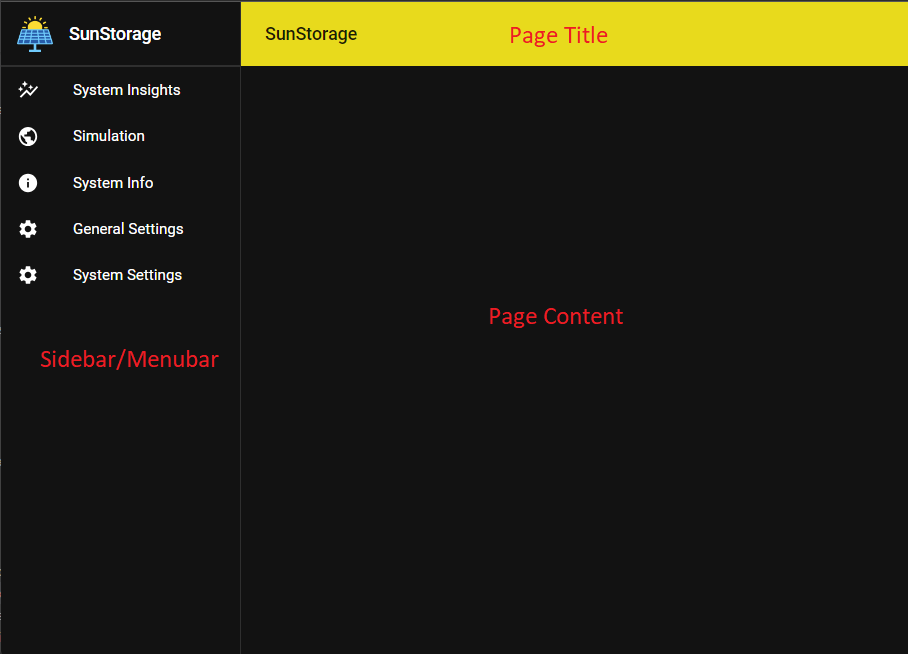
\includegraphics[width=\textwidth,keepaspectratio=true]{pics/Screenshot_Frontend_Design.png}
    \caption{Screenshot des Frontend Design}
    \label{fig:ScreenshotFrontendDesign}
\end{figure}

Wie in \autoref{fig:ScreenshotFrontendDesign} erkennbar, besteht das Frontend aus mehreren grundlegenden Komponenten. „Page Content“ ist die zentrale Komponente der Webseite  und zeigt die aktuell aufgerufene Seite an. „Page Title“ zeigt den Titel der Seite.
In „Sidebar/Menubar“ können die verschiedenen Seiten ausgewählt werden.
Dieses Menü verkleinert sich zu einem seitlich eingeschobenen Menü für kleine Displaybreiten und kann über einen Burger Button aufgerufen werden.
Das Menü bietet zudem die Funktion, je nach angezeigter Seite ein Untermenü einzubinden, um den „Page Content“ zu entlasten.
Dies ist vor allem für die in \autoref{websim} beschriebene Simulation wichtig.

\begin{figure}[htpb] % {H}
    \centering
    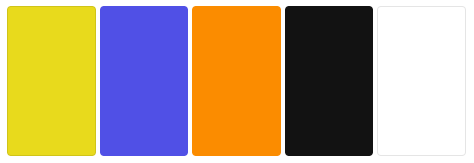
\includegraphics[width=\textwidth,keepaspectratio=true]{pics/Color_Palette_Frontend.png}
    \caption{Farbpalette}
    \label{fig:ScreenshotFrontendDesignColorPalette}
\end{figure}

Die Farbwahl (\autoref{fig:ScreenshotFrontendDesignColorPalette}) wurde passend zum Projektthema mit dem Spruch „Licht, das die Nacht erhellt“ als Kernthema entworfen. Ein mattes Gelb wurde somit als Primärfarbe gemeinsam mit einem dunklen Hintergrund definiert. Gelb als Farbe steht sowohl für die Sonne am Himmel, die auf das SolarPanel scheint als auch für den von unserem Gerät produzierten Strom. Eine nicht zu helle, matte Farbe zu wählen ist bei einem dunklen Hintergrund wichtig, damit kein stechender, greller Effekt für die Augen des Nutzers entsteht und komfortabel betrachtet werden kann.
Für die Schrift wurden Komplementärfarben zum aktuellen Hintergrund basierend auf der Farbpalette in \autoref{fig:ScreenshotFrontendDesignColorPalette} dargestellten verwendet. Ein mattes Lila als Sekundärfarbe zieht die Aufmerksamkeit des Nutzers nicht von den wichtigen Elementen der Seite weg und ist gut zu erkennen auf dem dunklen Hintergrund. Als abschließender Farbton wurde ein weiches Orange verwendet. Diese Farbe soll nur als weitere Option dienen, falls die Primär und Sekundäroptionen nicht ausreichen. Sie ist etwas intensiver als die Sekundärfarbe.

\subsubsection{Konfigurationsmöglichkeiten}
\chapterauthor{Valentin Weiß}

\begin{figure}[htpb] % {H}
    \centering
    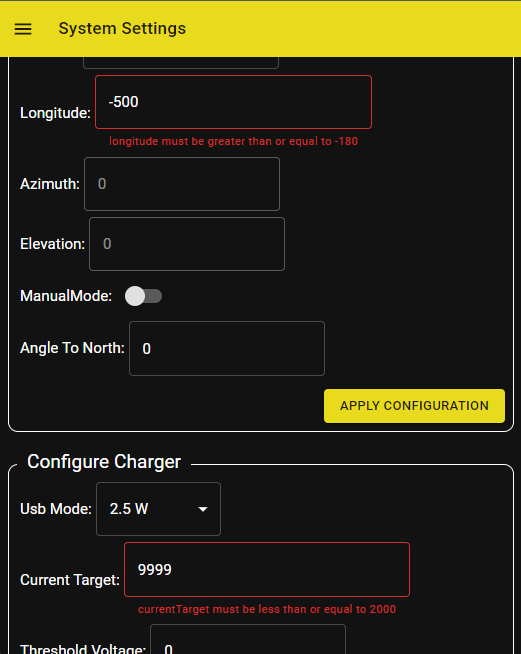
\includegraphics[height=12cm,width=\textwidth,keepaspectratio=true]{pics/Screenshot_SystemSettings.png}
    \caption{Screenshot der System Settings}
\end{figure}

Eine Kernfunktionalität ist die Konfiguration des SunStorage Systems. Hier bietet das Web-Frontend gruppenbasiert verschiedenste Konfigurationsmöglichkeiten zu folgenden Themen:
\begin{itemize}
    \item Positionierung und Panelausrichtung
    \item Ladegerät und Batterie
    \item Nachtabschaltung
    \item Display
    \item Stromsparen und zeitweise Abschaltung von Funktionen
    \item WiFi Konfiguration
\end{itemize}

Eingaben werden hier, wie auch auf allen anderen Seiten, auf Validität geprüft, um Datenintegrität zu gewährleisten und Missbrauch sowie potenziell gefährliche Konfigurationen zu vermeiden.
WiFi und Display werden nicht weiter aufgeführt.

\begin{table}[H]
    \begin{center}
      \begin{tabular}{|l|r|r|}
        \hline
        Wert          & Validierung & Beschreibung\\
        \Xhline{3\arrayrulewidth}
        Usb Mode & [0, 1, 2] & 0: 2.5 W; 1: 5 W; 2: 10 W \\
        \hline
        Current Target      & [0..2000]   & Wert in mA \\
        \hline
        Threshold Voltage   & [0..1000] & Wert in mV \\
        \hline
        Maximum Voltage   & [3800..4200] & Wert in mV \\
        \hline
        Trickle Threshold   & [3000..4200] & Wert in mV \\
        \hline
        Battery Size   & [0..10000] & Wert in mAh \\
        \hline
        Overheated Temperature   & [20..60] & Wert in Grad Celsius \\
        \hline
        High Power Enabled   & [true, false] &  \\
        \hline
        Overheated Hysteresis   & [1..10] & Wert in Kelvin \\
        \hline
      \end{tabular}
      \caption{Validierung Konfiguration Ladegerät}
    \end{center}
  \end{table}

  \begin{table}[H]
    \begin{center}
      \begin{tabular}{|l|r|r|}
        \hline
        Wert          & Validierung & Beschreibung\\
        \Xhline{3\arrayrulewidth}
        Enabled & [true, false] &  \\
        \hline
        Azimuth      & [0..360]   & Winkelgrad \\
        \hline
        Elevation   & [0..90] & Winkelgrad \\
        \hline
      \end{tabular}
      \caption{Validierung Konfiguration Nachtabschaltung}
    \end{center}
  \end{table}

  \begin{table}[H]
    \begin{center}
      \begin{tabular}{|l|r|r|}
        \hline
        Wert          & Validierung & Beschreibung\\
        \Xhline{3\arrayrulewidth}
        manualMode & [true, false] & Manuelle oder Automatische Panel Ausrichtung \\
        \hline
        Azimuth      & [0..360]   & Winkelgrad \\
        \hline
        Elevation   & [0..90] & Winkelgrad \\
        \hline
        Latitude   & [-90..90] & Breitengrad \\
        \hline
        Longitude   & [-180..180] & Längengrad \\
        \hline
        Angle To North   & [0..360] & Winkelgrad \\
        \hline
      \end{tabular}
      \caption{Validierung Konfiguration Positionierung}
    \end{center}
  \end{table}

  \begin{table}[H]
    \begin{center}
      \begin{tabular}{|l|r|r|}
        \hline
        Wert          & Validierung & Beschreibung\\
        \Xhline{3\arrayrulewidth}
        HTTP & [0..] & in Sekunden \\
        \hline
        GPS & [0..] & in Sekunden \\
        \hline
        WiFi & [0..] & in Sekunden \\
        \hline
        DCF-77 & [0..] & in Sekunden \\
        \hline
      \end{tabular}
      \caption{Validierung Konfiguration Funktionsabschaltung}
    \end{center}
  \end{table}

Eine Verbesserung der Displaykonfiguration wäre gewesen, wenn man nicht nur verschiedene Werte auf dem Display aktivieren und deaktivieren, sondern auch die Reihenfolge anpassen könnte. Dies wird jedoch von der API nicht unterstützt.

\subsubsection{System Insights}
\chapterauthor{Valentin Weiß}

\begin{figure}[htpb] % {H}
    \begin{center}
    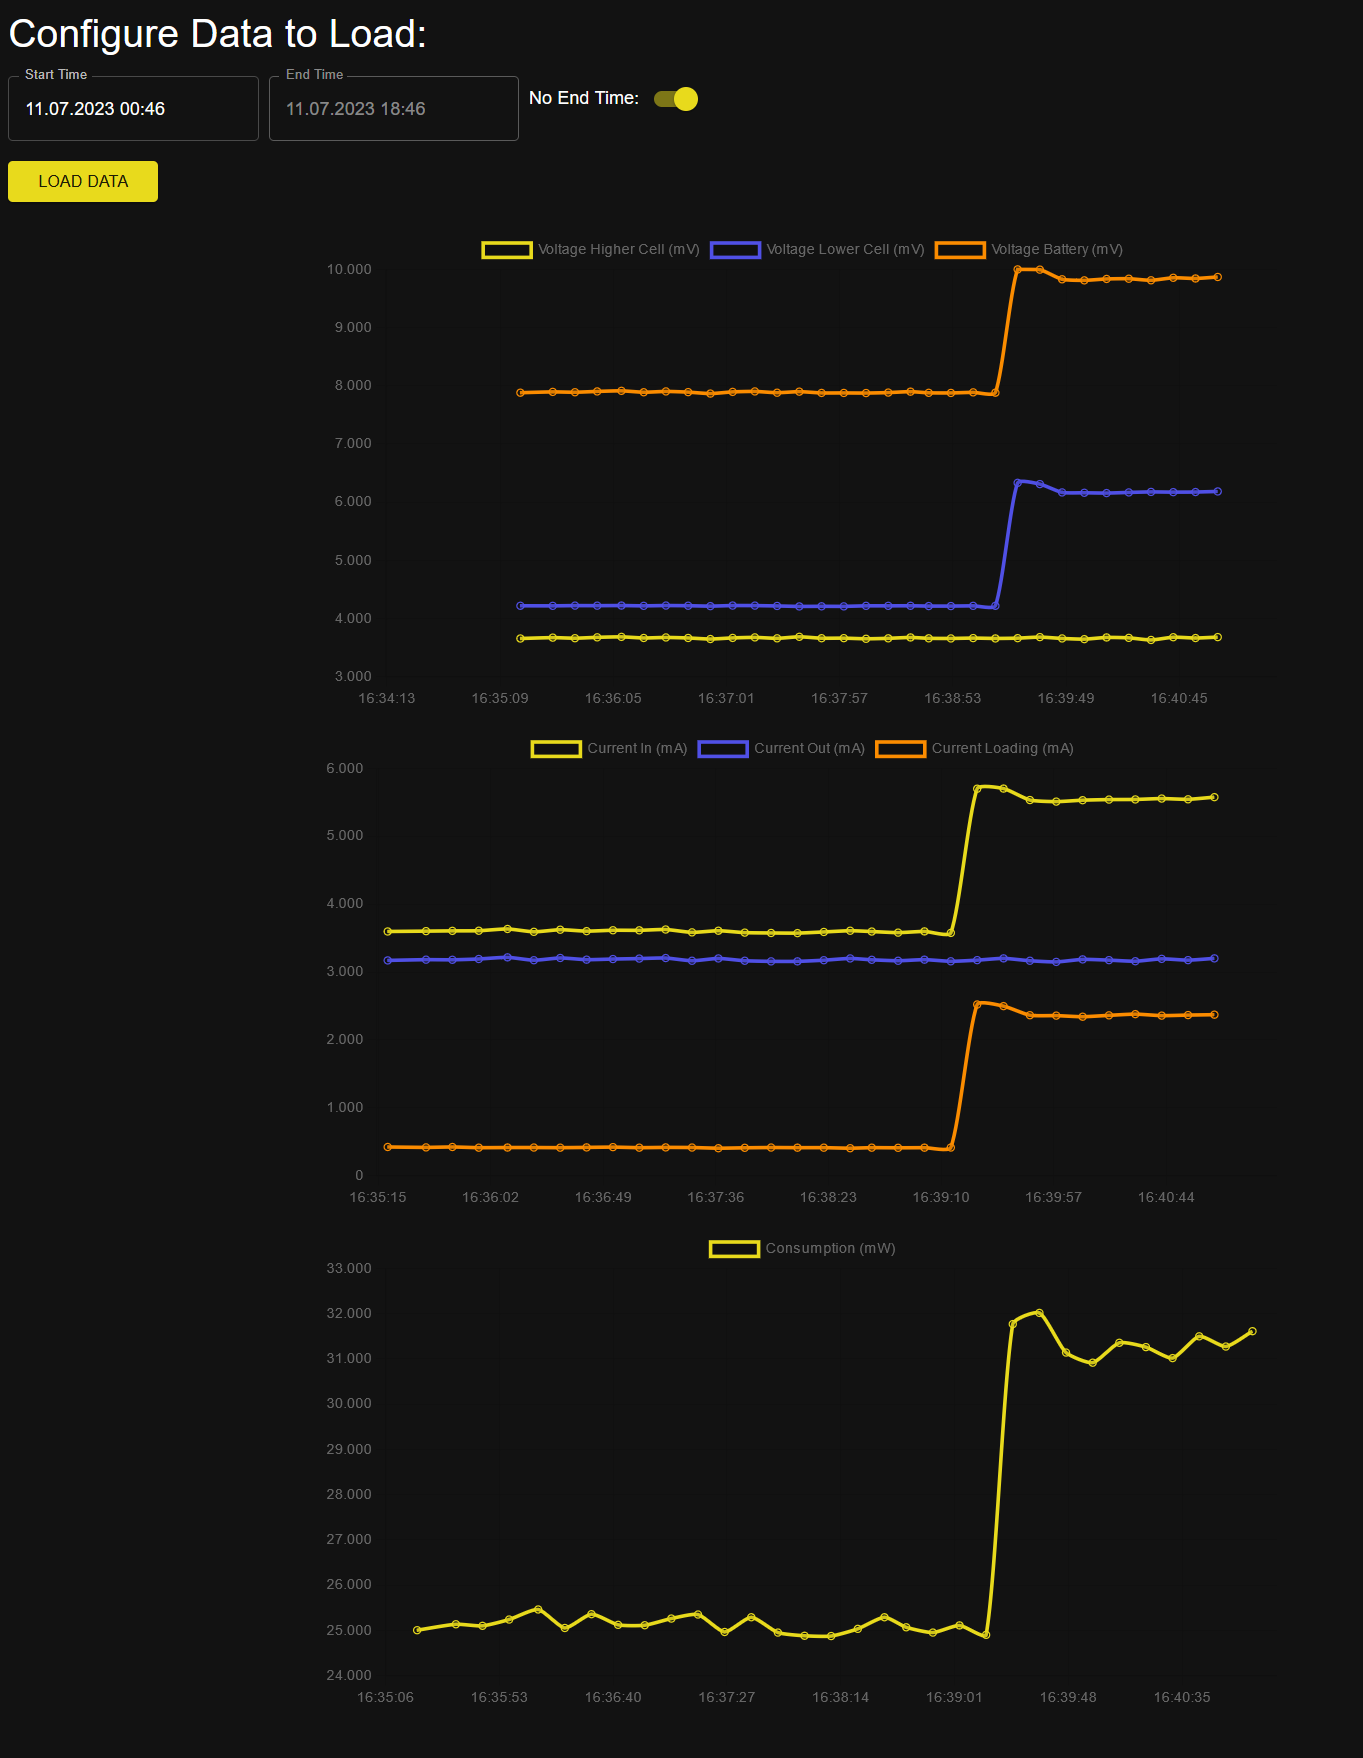
\includegraphics[width=10cm,keepaspectratio=true]{pics/Screenshot_ApplicationInsights.png}
    \caption{Screenshot der System Insights}
    \label{fig:systeminsights}
	\end{center}
    Der Sprung in den Werten entsteht durch das in die Sonne stellen.
   	In den finalen Einstellungen ist die Abtastrate wesentlich niedriger.
   	Auf die Richtigkeit der Werte wird in Kapitel \autoref{akkuCircuit} eingegangen.
   	Durch Messungen stellte sich heraus, dass der Bipolartransistor zur Steuerung des Ladestroms kaputt ist.
   	Daher wird der Ladestrom nicht gesteuert.
\end{figure}

Diese Seite bietet, wie in \autoref{fig:systeminsights} gezeigt, die Möglichkeit Systemdaten über einen Zeitbereich auszulesen und sie graphisch darzustellen.
Hier können entweder Datensätze über einen Zeitbereich zwischen einer Start- und Endzeit oder zwischen Startzeit und dem neusten verfügbaren Datensatz ausgelesen werden.
Es werden drei Graphen gebildet:
\begin{enumerate}
    \item Graph für Spannungsinformationen
    \item Graph für Strominformationen
    \item Graph für Leistungsinformationen
\end{enumerate}

Dies wurde mittels der react-chartjs-2 Bibliothek umgesetzt, die eine React Implementierung für das chart.js Framework bietet.

\subsubsection{Ungenutzte Erweiterungen}
\chapterauthor{Valentin Weiß}
Da das Frontend schon sehr früh im Projekt implementiert wurde, sind später Funktionalitäten hinzugefügt worden, welche die User-Experience weiter verbessern.
Aus zeitlichen Gründen konnten diese nicht im Backend umgesetzt werden.
Dies beinhalteten hauptsächlich das Streaming von Informationen.
Hierfür wurden zwei ungenutzte Technologien implementiert.

\paragraph{HTTP SSE (Server-Sent Events)}
\chapterauthor{Valentin Weiß}

SSE bietet die Möglichkeit über offene HTTP Verbindungen Daten vom Server zum Client zu senden.
Hier wäre es möglich gewesen, aktuelle Datenänderungen direkt an das Frontend zu streamen, ohne dass ein Client Änderungen anfragen muss.
Eine Entlastung des ESP kommt hier zustande, wenn mehrere Frontendinstanzen die gleichen Daten regelmäßig abfragen, um möglichst aktuell zu bleiben.
Hiermit könnte man beispielsweise in Application Insights Diagramme erstellen, die die neusten Werteveränderungen über die Zeit direkt anzeigen.

\paragraph{MQTT (Message Queuing Telemetry Transport)}
\chapterauthor{Valentin Weiß}
Die MQTT Implementierung hätte ähnlich wie SSE verwendet werden können, um im Frontend mit aktuellen Daten zu arbeiten, ohne den ESP weiter zu belasten.
Der ESP sendet die neuen Daten an einen Broker, welcher die Verteilung von Daten übernimmt.
Dadurch wäre der ESP von Anfragen entlastet, da diese der Broker als externes Gerät übernimmt.
Besonders dann, wenn mehrere Frontend-Clients gleichzeitig verwendet werden.
Diese Technologie gilt als Standard im IoT Bereich \autocite{front:mqtt}.

\paragraph{Web Logging}
\chapterauthor{Valentin Weiß}
Durch eine SSE oder MQTT Realisierung wäre es möglich das umgesetzte Web Logging zu verwenden.
Hier hätten Log Nachrichten des ESP live ausgelesen und angezeigt werden können, was beim Debugging hilfreich gewesen wäre.
Durch die Belegung eines UART Ports des ESP durch das GPS Modul muss nach dem Zusammenbau des Projekts muss das Logging über UART deaktiviert sein.
Besonders in dieser letzten Phase des Projekts wäre das Web Logging hilfreich gewesen.
Eine weitere Möglichkeit ist, ein Logfile auf der SD-Karte des ESP zu erzeugen, um die Daten per HTTP auszulesen.
Auch diese Funktion wird vom ESP aktuell nicht unterstützt.

\subsubsection{Fazit}
\chapterauthor{Valentin Weiß}
Insgesamt war es sehr interessant das Web-Frontend zu planen und zu Implementieren.
Ich habe nun ein guts Verständnis von React Anwendungen und habe mein bisheriges Wissen in den Webtechnologien weiter vertieft.
Da dieses Framework doch sehr anders funktioniert als bisher benutzte Technologien habe ich länger als geplant zur Einarbeitung und zum Lernen der Umgebung benötigt.
Neue Konzepte wie React Context, Hooks oder die komponentenbasierte Projektverwaltung sind sehr interessant.

Vergleichsweise häufige API Änderungen verursachten zusätzlichen Zeitaufwand, welcher durch mehr Kommunikation und Planung vermeidbar gewesen wäre.
Obwohl viel Code am Ende ungenutzt bleibt, hat mich die Einarbeitung in MQTT und SSE persönlich weitergebracht.

Insgesamt bin ich zufrieden mit dem Ergebnis des Web-Frontend.

\subsection{Simulation des Panels im Frontend}\label{websim}
\chapterauthor{Valentin Weiß}
Das Web-Frontend soll dem Nutzer die Möglichkeit bieten, über eine 3D Simulation die Sonnenposition und Panelausrichtung darzustellen, damit sich der Nutzer die Ausrichtung und Zusammenhänge besser vorstellen kann.

\subsubsection{Sky Dome Model}
\chapterauthor{Valentin Weiß}
Wegen der großen Entfernung der Sonne zur Erde von knapp 150 Millionen Kilometern wird die Sonne nur als helle, kleine Kreisfläche wahrgenommen.
In einem Kuppelmodell (Sky Dome Model) machen wir uns das zu nutze (\autoref{fig:DomeModel}).
In diesem Modell wird eine Position auf der Erde annähernd als Kreisfläche dargestellt. Die Sonne (oder auch andere Objekte im Weltall) wird hier in konstanter Distanz auf der Kuppel in der echten Richtung dargestellt. Dies ist natürlich von verschiedenen Faktoren wie Ort und Zeit abhängig.

\begin{figure}[htpb] % {H}
    \centering
    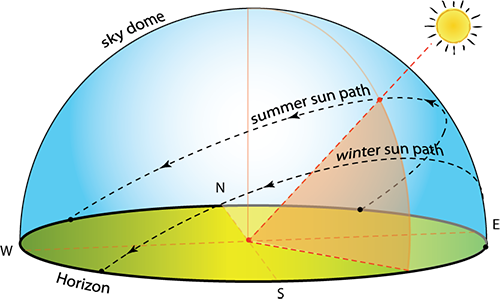
\includegraphics[width=\textwidth,keepaspectratio=true]{pics/SkyDomeModel.png}
    \caption{Simulation Model: SkyDome \autocite{front:SkyDome:img}}
    \label{fig:DomeModel}
\end{figure}

\subsubsection{Algorithmus Sonnenposition}

\paragraph{Grundlegender Algorithmus}
\chapterauthor{Valentin Weiß}

Für die Simulation, aber auch für die automatische, optimale Panelausrichtung auf dem ESP muss die Position der Sonne berechnet werden.
Wie im Simulationsmodell (\autoref{fig:DomeModel}) gezeigt, muss der Drehwinkel (Azimut) sowie der Steigungswinkel (Elevation) zur Sonne über einen Algorithmus berechnet werden.

Azimut ist hierbei der Drehwinkel auf durch die Erdoberfläche dargestellten Ebene.
Dieser zeigt mit $0\degree$ Richtung Norden und dreht sich bei steigenden Werten gegen den Uhrzeigersinn. Beispielsweise zeigt ein Azimut von $90\degree$ Richtung Westen. Der Wertebereich des Azimut liegt somit bei $[0\degree; 360\degree]$ \autocite{front:AzimuthAngle}.

Elevation ist der Winkel, der aussagt, wie weit die Sonne über oder unter dem Horizont steht. In Abbildung \ref{fig:DomeModel} ist dieser Winkel in der Farbe orange eingetragen.
Ein Winkel größer als $0\degree$ sagt aus, dass die aktuelle Position beleuchtet ist (Tag). Ein Winkel kleiner als $0\degree$ bedeutet, dass die Sonne die aktuelle Position nicht beleuchtet (Nacht).
Beispielsweise repräsentiert $0\degree$ den Sonnenaufgang oder Sonnenuntergang.
$90\degree$ beschreibt, dass die Sonne direkt über der aktuellen Position ist.
Der Wertebereich der Elevation liegt somit bei $[-90\degree; 90\degree]$ \autocite{front:ElevationAngle}.

Die Sonnenposition an gewissen Koordinaten ist abhängig von der Erdrotation zur Sonne.
Diese kann durch den Stundenwinkel $HRA$ (Hour Angle) an einer Position bzw. gewissen Koordinaten dargestellt werden.
Der Stundenwinkel $HRA$ ist der Verlauf der Sonne, den man an einem gewissen Tag an einer gewissen Position wahrnimmt.
Dabei wird der höchste Stand der Sonne (Solar Noon) mit $0\degree$ definiert. Durch die Drehung der Erde von $15\degree$ pro Stunde ($\frac{360\degree}{24h} = \frac{15\degree}{1h}$), ändert sich auch der Stundenwinkel pro Stunde um diesen Wert. Ein negativer Winkel repräsentiert einen Winkel vor dem Höchststand der Sonne, ein positiver einen Winkel nach dem Höchststand der Sonne. Beispielsweise ist ein $HRA$ Winkel von $-45\degree$ einer Zeit 3 Stunden vor dem Sonnenhöchststand zugeschrieben \autocite{front:SolarTime}.

Die lokale Sonnenzeit $LST$ (Local Solar Time) bestimmt mit der Uhrzeit 12:00 Uhr genau diesen Winkel ($HRA = 0\degree$) und somit eine einfache Berechnung des Winkels:

\[ HRA = 15\degree*(LST - 12) \]

Der Sonnenhöchststand ist etwa Mittags $LT$ (lokale Zeit/Local Time), jedoch muss es aufgrund der Ungenauigkeit der Zeitzonen gegenüber der Position im Längengrad ($TCLongitude$) und der Ungenauigkeit der Erdumlaufbahn zur Sonne inklusive Achsenwinkel ($TCEoT$) ein zeitlicher Korrekturfaktor in Minuten $TC$ (Time Correction Factor) zur $LT$ addiert werden, um die $LST$ zu berechnen.

\[ LST = LT + \frac{TCLongitude + TCEoT}{60} \]

\[ TCLongitude = \frac{4min}{1\degree}*(Longitude - (\frac{15\degree}{1h} * T_{UTC})) \]

Wobei sich die Erde um 15 Grad pro Stunde und folgend um 1 Grad alle 4 Minuten dreht. $T_{UTC}$ ist die Zeitzone, in der man sich befindet in Stunden abhängig von der koordinierten Weltzeit $UTC$ (Coordinated Universal Time). Für Deutschland ist diese Zeitzone im Winter MEZ ($UTC+1$) und im Sommer MESZ ($UTC+2$).

\[ TCEoT = 9.87sin(2B) - 7.53cos(B) - 1.5sin(B) \]

Wobei

\[ B = \frac{360\degree}{365\,days\,per\,Year}*(d - 81) \]

$d$ ist hierbei der Tag im aktuellen Jahr ab dem ersten Januar. $81$ ist der 81te Tag im Jahr, also der 22. März. An diesem Tag steht die Erde zur Sonne im Neigungswinkel $0\degree$ (\autoref{fig:DeclinationAngleFigure}). Je nach Schaltjahr könnte hier ein genauerer Wert verwendet werden, jedoch ist die $TCEoT$ (Equasion of Time) Abweichung so gering, dass das dies nur einen geringen Einfluss auf mehrere Nachkommastellen hätte, wordurch dies zu vernachlässigen ist. Der durch diese empirische Gleichung berechnete Wert ($TCEoT$) auch nur eine Annäherung die auf etwa eine halbe Minute genau ist.

\begin{figure}[htpb] % {H}
    \centering
    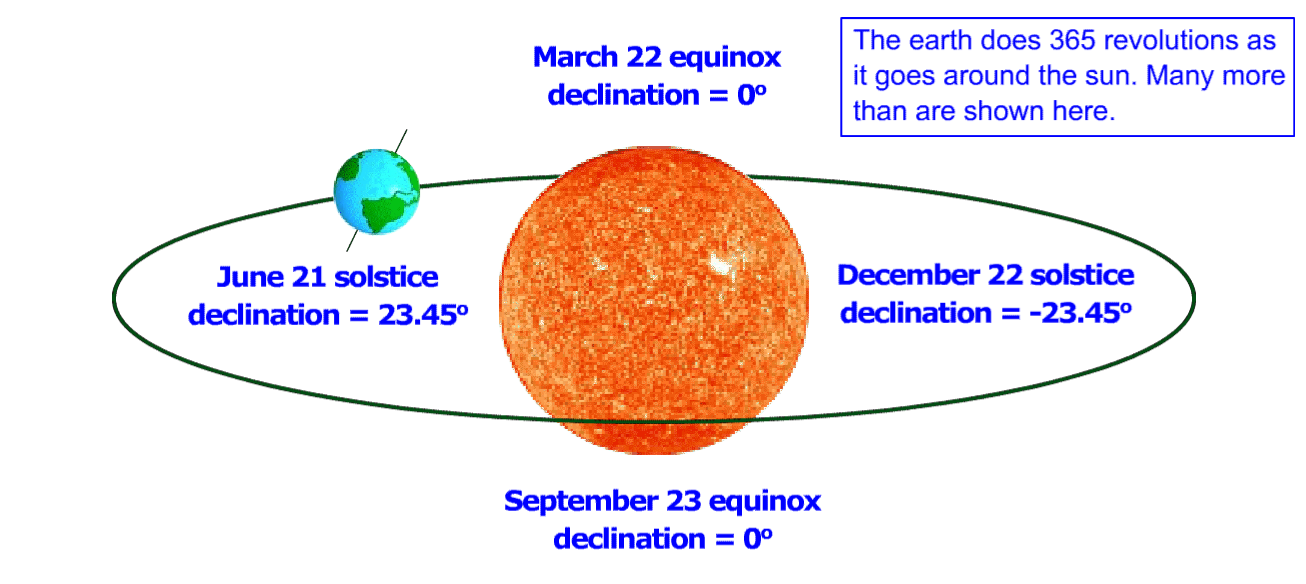
\includegraphics[width=\textwidth,keepaspectratio=true]{pics/DeclinationAngleEarthSun.png}
    \caption{Darstellung des Erdwinkel zur Sonne \autocite{front:DeclinationAngle}}
    \label{fig:DeclinationAngleFigure}
\end{figure}

\begin{figure}[htpb] % {H}
    \centering
    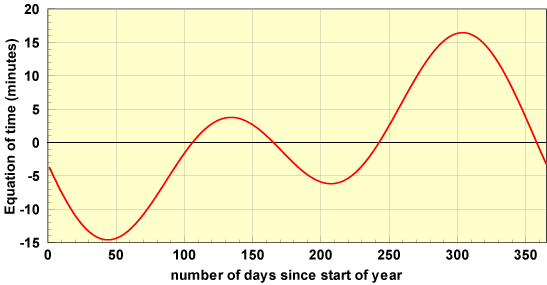
\includegraphics[width=\textwidth,keepaspectratio=true]{pics/TCEoT.png}
    \caption{Darstellung der Werte von $TCEoT$ über das Jahr \autocite{front:SolarTime}}
    \label{fig:TCEoT}
\end{figure}

Nachdem nun der $HRA$ Wert berechnet werden kann, muss die Neigung der Erdkugel zur Sonne noch berücksichtigt werden. Diese Neigung $\delta$ berechnet sich aus der maximalen Erdneigung von $23.45\degree$ in Kombination mit einer Sinusfunktion der bereits zuvor erklärten $0\degree$ Neigung am 22. März \autocite{front:DeclinationAngle}.

\[ \delta = 23.45\degree * sin(B) \]

$\delta$ kann als eine nördliche/südliche Äquator-Verschiebung gesehen werden, an der die Sonne im Elevationswinkel von $90\degree$ zur $LST$ 12:00 Uhr scheint.

$Azimut$ und $Elevation$ berechnen sich durch die kombination der zuvor berrechneten Werte:

\[ Elevation = sin^{-1} \left[sin(\delta)*sin(Latitude) + cos(\delta)*cos(Latitude)*cos(HRA)\right] \]

\[ Azimut = cos^{-1} \left[\frac{sin(\delta)*cos(Latitude) - cos(\delta)*sin(Latitude)*cos(HRA)}{cos(Elevation)}\right] \]

Die obere Berechnung gibt den korrekten Wert nur für Zeiten vor dem Höchststand der Sonne. Für den fall, dass $HRA > 0$ oder $LST > 12$ muss der $Azimut$ von $360\degree$ abgezogen werden.

\[ Azimut = 360\degree - Azimut \]

\paragraph{Verbesserungen den Algorithmus für die Simulation}
\chapterauthor{Valentin Weiß}

Der Algorithmus funktioniert gut, um eine statische Sonnenposition zu berechnen, jedoch hat dieser Probleme, wenn es darum geht die Sonne zu simulieren, da vor allem beim Übergang der Animation von einem Tag zum darauffolgenden unschöne Sprünge der Sonne auftreten können.

\begin{enumerate}
    \item Bei der Berechnung des Tags im aktuellen Jahr wurden statt Ganzzahlen nun Fließkommazahlen verwendet. Die verringert Sprünge in der Position beim Anbruch eines neuen Tages.
    \item Es kann vorkommen, dass die $LST$ negativ ist, in der Nähe der Mitternachtszeit. Dies tritt beispielsweise auf, wenn der berechnete zeitliche Korrekturfaktor $TC$ negativ ist und $LT$ klein ist (neuer Tag). Deshalb wird der Wert $LST$ auf das Intervall $[0h; 24h]$ normalisiert nach der Berechnung.
    \item Der Winkel $HRA$ verursacht auch Probleme der gleichen Art. Auch dieser musste auf ein festes Intervall von $[-180\degree; 180\degree]$ normalisiert werden.
\end{enumerate}

Durch diese Verbesserungen ist es möglich, die Sonne in der Simulation durchwegs flüssig und ohne Sprünge zu animieren.

\subsubsection{Positionierung im 3D-Raum}
\chapterauthor{Valentin Weiß}

Um das Simulationsmodell Sky Dome zu realisieren, muss zunächst ein 3D-Raum definiert werden. Da der Beobachter der Simulation bzw. das SolarPanel immer ein Eckpunkt der folgenden Berechnungen sein wird, ist es sinnvoll diesen an den Ursprung der Simulation zu positionieren. So sind die Koordinaten eines Punktes auch immer der Vektor vom Ursprung zum Punkt. Ein Punkt in diesem 3D-Raum $P(x,y,z)$ soll folgendermaßen definiert sein:
\begin{itemize}
    \item $x$ Achse: West-Ost Achse im Sky Dome Model. Mit $x < 0$ Westrichtung und $x > 0$ Ostrichtung.
    \item $y$ Achse: Oben-Unten Achse im Sky Dome Model. Mit $y < 0$ als „Unten“ und $y > 0$ als „Oben/Himmel“.
    \item $z$ Achse: Nord-Süd Achse im Sky Dome Model. Mit $z < 0$ Nordrichtung und $z > 0$ Südrichtung.
\end{itemize}

\paragraph{Sonnenposition im 3D-Raum}
\chapterauthor{Valentin Weiß}

Eine der wichtigsten Funktionen der Simulation ist, die Sonne anhand den berechneten Winkeln Azimut und Elevation richtig zu positionieren. Ein Vektor der Länge 1 würde mit den Winkeln $Azimut = 0\degree$ und $Elevation = 0\degree$ nach obriger Definition folgendermaßen aussehen:

\[
\mathbf{v} = \begin{bmatrix}
x \\
y \\
z \\
\end{bmatrix}
=
\begin{bmatrix}
0 \\
0 \\
-1 \\
\end{bmatrix}
\]

Dieser Vektor zeigt also eine Einheit Richtung Norden. Um die Richtung dieses Vektors anhand beliebiger Winkel für $Azimut$ und $Elevation$ anzupassen, muss der Vektor anhand der für den $Azimut$ Winkel an der y-Achse gegen den Uhrzeigersinn gedreht werden. Anschließend für den $Elevation$ Winkel an der daraus resultierenden Senkrechten durch den Ursprung. Um dies Programmtechnisch einfacher und ohne mehrmalige Rotationsmatrizen umzusetzen wurde der Fakt genommen, der oben genannte Eingangsvektor bekannt ist und am Ursprung anliegt, um dies mit einfachen Trigonometrischen Funktionen zu lösen.

\[
\mathbf{v} = \begin{bmatrix}
x \\
y \\
z \\
\end{bmatrix}
=
\begin{bmatrix}
cos(elevation) * sin(azimut) * -1 \\
sin(elevation) \\
cos(elevation) * cos(azimut) * -1 \\
\end{bmatrix}
\]

Dieser repräsentiert nun einen Vektor der Länge 1, der in Richtung der Sonne zeigt. Dieser kann jetzt einfach mit einer Konstante multipliziert werden, um als Punkt gesehen die Koordinaten der Sonne in Entfernung der Konstanten zu bestimmen.

\paragraph{SolarPanel Ausrichtung und Effizienzberechnung}
\chapterauthor{Valentin Weiß}

Die SolarPanel Ausrichtung erfolgt wie bei der Sonne über die Winkel $Azimut$ und $Elevation$. Hier muss nur anschließend die Höhe der Panel-Halterung auf den y-Wert addiert werden, damit das Panel durch die Höhe der Halterung keine Ungenauigkeit bekommt. Um die Form in Richtung Sonne zeigen zu lassen sind keine weiteren Berechnungen nötig, da diese Funktion bereits in der Three.js Bibliothek existiert.

Die Effizienzberechnung in der Simulation ist eine rein ausgedachte Methode, kann aber annähernd als guter Referenzwert angenommen werden.
Sei $\mathbf{v}_{\mathrm{1}}$ der Vektor zur Sonnenposition und $\mathbf{v}_{\mathrm{2}}$ die Blickrichtung des SolarPanels, dann ist der Winkel $\alpha$ zwischen den beiden Vektoren:

\[
\alpha = \cos^{-1} \left[\frac{\mathbf{v}_{1} \cdot \mathbf{v}_{2}}{|\mathbf{v}_{1}| \cdot |\mathbf{v}_{2}|}\right]
\]

Dann ist die Effizienz des SolarPanels wenn $\alpha < 90\degree$ und $Elevation > 0$

\[
Effizienz = cos(\alpha) * 100\%
\]

an sonsten $0\%$. Somit bringt das SolarPanel bei kleinen Winkelverschiebungen immer noch hohe Effizienzwerte, ist jedoch nach Sonnenuntergang bzw. ab einem abweichenden Winkel von über $90\degree$ $0\%$, da keine aktive Beleuchtung nicht mehr stattfindet.

\subsubsection{Umsetzung der Simulation}

\paragraph{Simulationsmenü}
\chapterauthor{Valentin Weiß}

Wie aus dem Algorithmus hervorgeht, werden verschiedene Parameter für die Simulation benötigt, um mit dem Algorithmus die Sonnenposition berechnen zu können.
Um diese Anforderungen visuell umzusetzen, ohne viel Platz für die Simulation zu verbrauchen, wurde ein Untermenü geschaffen, welches das eigentliche Menü mit Funktionen erweitert. Der Datenaustausch zwischen Simulation und Menü erfolgt über einen React Context.

Einstellungen Zur Berechnung der Sonnenposition in diesem Modell sind:
\begin{itemize}
    \item Längengrad und Breitengrad: Die Sonnenposition ist abhängig davon wo man sich auf der Erdkugel befindet. Je nach Position kann es verschiedene Sonnenstände zur gleichen Uhrzeit geben.
    \item Datum: Über das Jahr gesehen (abhängig von der Erdwinkel zur Sonne) verändert sich die Sonnenposition.
    \item Uhrzeit + Zeitzone: Die Erdrotation zur Sonne ist abhängig von Uhrzeit und Zeitzone.
\end{itemize}

Einstellungen zur Position des SolarPanels in der Simulation:
\begin{itemize}
    \item Azimut Winkel: Winkel zur Rotation des SolarPanels am Boden.
    \item Elevation Winkel: Winkel zur Neigung des SolarPanels.
    \item "Best Panel Angle": Diese Option deaktiviert die Bearbeitung von Azimut und Elevation. Diese Felder werden automatisch mit den optimalen Stand zur Sonne gefüllt.
\end{itemize}

Simulationsanimation:
\begin{itemize}
    \item „Animation Speed“: Wenn in diesem Feld eine Zahl steht, wird pro Sekunde in Simulationszeit die Sonne um X Minuten simuliert. Beispielwert 60: Pro Sekunde Simulation = 1 Stunde Sonnenverschiebung. Auch negative Werte sind möglich.
\end{itemize}

 Über die „Show Simulation Info“ Option werden live Werte der Sonnenberechung sowie die berechnete Effizienz des SolarPanel ausgegeben.

 \begin{figure}[htpb] % {H}
    \centering
    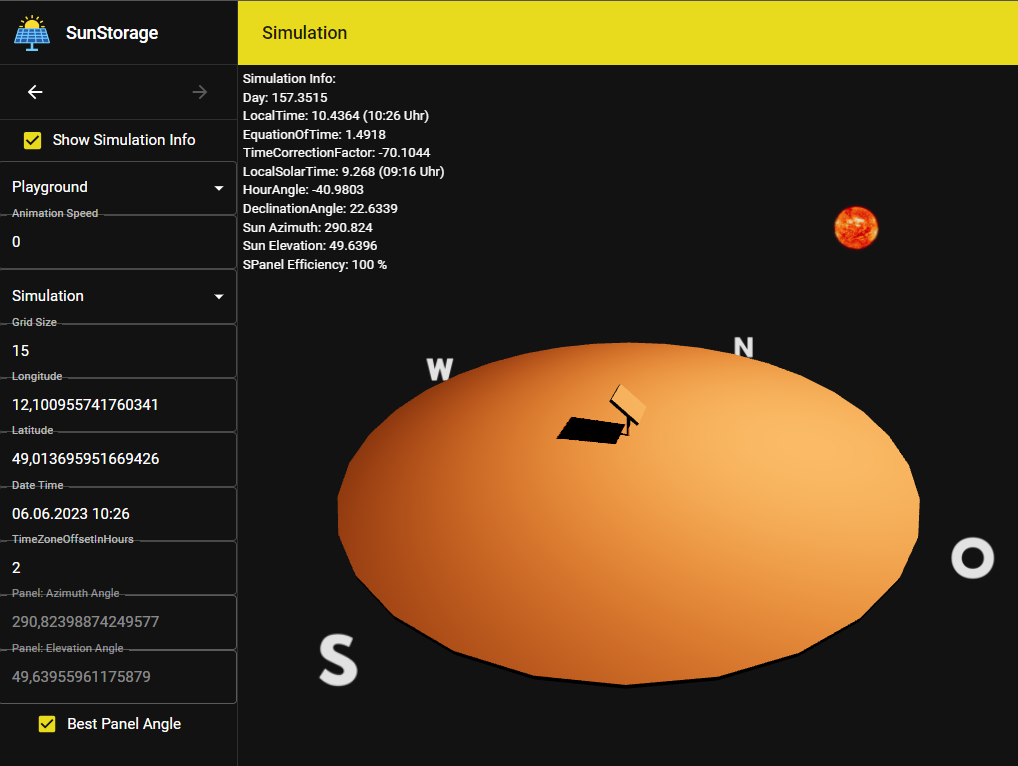
\includegraphics[width=\textwidth,keepaspectratio=true]{pics/Screenshot_WebUI_Simulation.png}
    \caption{Screenshot des Simulation Playground}
    \label{fig:SimulationScreenshotPlayground}
\end{figure}

\begin{figure}[htpb] % {H}
    \centering
    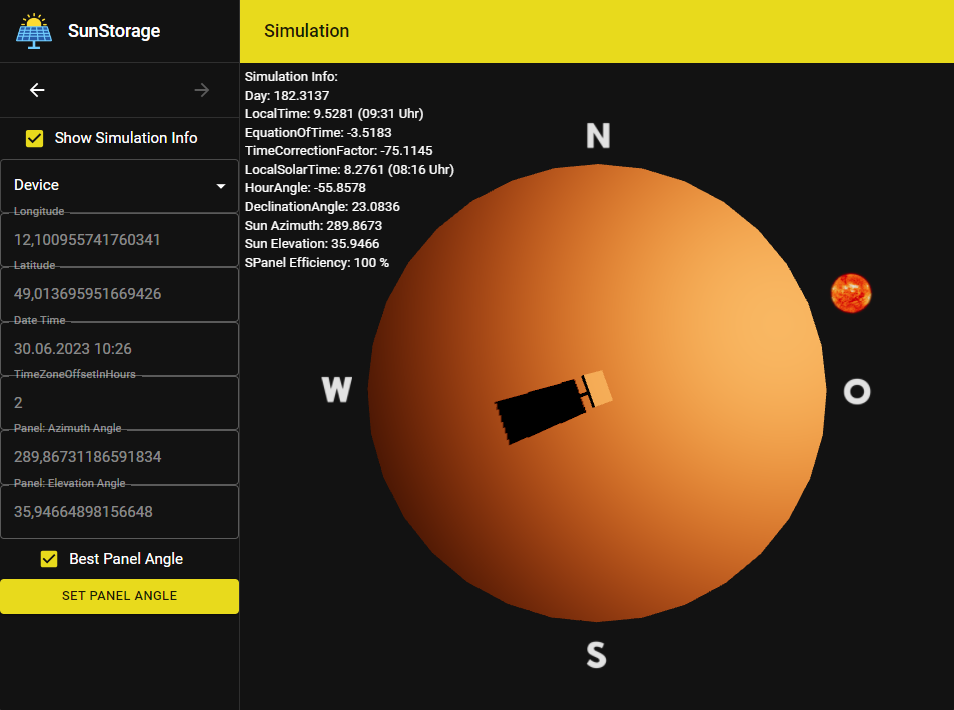
\includegraphics[width=\textwidth,keepaspectratio=true]{pics/Screenshot_WebUI_Simulation_Device.png}
    \caption{Screenshot des Simulation Device}
    \label{fig:SimulationScreenshotDevice}
\end{figure}

 Es wurden 2 Modi für die Konfiguration geschaffen.
 Im Modus Playground (Abbildung \ref{fig:SimulationScreenshotPlayground}) sind erweiterte Einstellungen für die Simulation möglich, wie beispielsweise die manuelle Eingabe der Koordinaten, der Zeit und Zeitzone sowie eine Option, die Zeit in beliebiger Geschwindigkeit zu animieren, um den Sonnenverlauf besser zu betrachten.
 Im Modus Device (Abbildung \ref{fig:SimulationScreenshotDevice}) ist nur die Einstellung des SolarPanel möglich, kombiniert mit einem zusätzlichen Button diese Konfiguration an das Gerät zu senden.

Eine weitere Verbesserung, die aufgrund von Zeitgründen nicht mehr implementiert wurde, ist das mit Einbeziehen des Standwinkels vom SunStorage Gerät, um eine Winkelkorrektur des SolarPanels zur Sonne an unebenen Flächen zu gewährleisten. Dies wurde nun nur auf dem ESP implementiert.

\paragraph{Simulationsanimation}
\chapterauthor{Valentin Weiß}

Die Simulation wurde mithilfe von Three.js implementiert. Three.js ist eine JavaScript-Bibliothek, die zum Erstellen und Anzeigen animierter 3D-Grafiken benutzt wird. Durch das Verwenden von WebGL wird die Grafikkarte angesteuert, um hohe Aktualisierungsraten und somit flüssige Animationen zu erstellen.
Um die Integration von Three.js in React zu erleichtern und zu erweitern, wurden folgende Bibliotheken verwendet:
\begin{itemize}
    \item @react-three/fiber: Ein React Renderer für Three.js
    \item @react-three/drei: Funktionserweiterungen und Abstraktionen von @react-three/fiber
\end{itemize}

\subsubsection{Fazit Simulation}
\chapterauthor{Valentin Weiß}

Insgesamt war die Simulation mein persönliches Highlight des ganzen Projekts. Eine interessante Kombination aus Mathematik und dem Arbeiten im 3D Raum. Obwohl ich viele Stunden in die Simulation gesteckt habe, war die Umsetzung doch einfacher als erwartet durch ein exzellentes Framework (Three.js) und hierfür bereits existierende Implementierungen und Erweiterungen für React Projekte.

Der Algorithmus zur Berechnung der Sonnenposition hat dafür länger als erwartet gedauert. Hierfür musste ich verschiedene Algorithmen, Quellen und Pakete untersuchen, welche oft nicht zum erwarteten Ergebnis geführt haben.


\subsection{Elektronik}
\chapterauthor{Lukas Eigenstetter}
Ein wichtiger Teil des Projektes war der Aufbau der Elektronik.\\
Diese umfasst zum einen die Stormversorgung der Controller und Sensoren.
Zusätzlich wurde ein Ladegerät, das den Strom vom Solar-Panel in den Akku steuert, entworfen.
Um eine genaue Regelung zu erlauben, mussten ein Messschaltkreis gebaut werden.
Da Strommessungen über Spannungsabfall an Shunts sehr ungenau sind, wurde zusätzlich ein Coulomb-Counter entworfen und verbaut.\\
In diesem Kapitel werden die umgesetzten Schaltkreise und deren Steuerung in Software erklärt.
Zusätzlich werden Probleme und Alternativen erklärt.\\
Die komplizierteren Schaltkreise wurden zunächst mit dem Falstad Circuit Simulator Applet getestet. \autocite{falstad}
Dies ist Umgebung, die ein einfaches Entwerfen und Testen erlaubt.
Die Abbildungen der Teilschaltpläne wurden auch mit dieser Software erstellt.

\subsubsection{Stromversorgung}
\chapterauthor{Lukas Eigenstetter}
Die Stromversorgung für Controller und Sensoren wird mittels eines Linearreglers realisiert.
Dieser reguliert die nicht konstante Batteriespannung, die im Bereich von 7 - 8.4 V liegen kann, auf einen konstanten Wert von 5 V.
Verbaut wurde ein Regler vom Typ 7805CV.\\
Die standardmäßige Schaltung sieht einen 330 nF Kondensator am Eingang V\_IN und einen 100 nF Kondensator am Ausgang vor. \autocite{linearregler}
Verbaut wurden Kunststofffolienkondenstoren.\\
Zusätzlich sind am Ein- und Ausgang 100 \textmu F Aluminium-Elektrolytkondensatoren verwendet.
Der Eingangskondensator dient dazu, Spannungserhöhungen- und Abfälle durch Veränderungen in der Batteriespannung abzufedern.
Durch den Ausgangskondensator werden Verbrauchsspitzen abgefedert.\\
Der Linearregler kann dauerhaft einen Ausgangsstrom von etwa 500 mA erzeugen.
Dieser Strom reicht zur Versorgung der Module und des Displays aus.\\
Tabelle \autoref{PowerConsumption} zeigt den gemessenen Verbrauch der Module.

\begin{table}[H]
    \begin{center}
        \begin{tabular}{|l|l|l|}
            \hline
            Modul                 & Stromverbrauch in mA       & Spannung in Volt \\
            \Xhline{3\arrayrulewidth}
            GPS                   & 100                        & 5.0              \\
            \hline
            Beschleunigungssensor & 0                          & 3.3              \\
            \hline
            Kompass               & 0                          & 3.3              \\
            \hline
            Display               & 0 - 5 (je nach Helligkeit) & 5.0              \\
            \hline
            SD-Card               & 40                         & 5.0              \\
            \hline
            Temperatursensor      & 0                          & 3.3              \\
            \hline
            ESP32                 & 40 - 60 (je nach Last)     & 5                \\
            \hline
        \end{tabular}
        \caption{Gemessener Stromverbrauch der Module\\
            Der gesamte Stromverbrauch liegt im Betrieb deutlich über 200 mA.}
        \label{PowerConsumption}
    \end{center}
\end{table}

Laut Datenblatt soll das GPS-Modul lediglich mit maximal 3.6 V versorgt werden.
Aufgrund des hohen Verbrauchs führt dies dazu, dass der Linearregler eines ESP32, der etwa 80 mA abgeben kann, nicht ausreicht.
Da das Modul einen USB Anschluss und einen eigenen Regler besitzt, ist es möglich auch 5 V zu verwenden.
Daher wurde dieses Modul ebenfalls an die 5 V Quelle angeschlossen.\\
Der hohe Stromverbrauch des Systems führt dazu, dass im realistischen Betrieb nur unter guten Wetterbedingungen mehr Strom produziert als verbraucht wird.
Um langfristig eine positive Energiebilanz zu erreichen, müssten Display, GPS und die weiteren Module ausschaltet und nur durch eine Nutzereingabe aktiviert werden.
Diese Verbesserung konnte nicht mehr realisiert werden.\\
Ein weiteres Problem bei der Stromversorgung ist die Verwendung zu dünner Kabel.
Alle Verbindungen wurden mittels der im Labor verfügbaren Jumperkabel realisiert.
Dies hat den Vorteil, dass die Sensoren für zukünftige Projekte weiter verwendet werden können.
Ein festes Verlöten der Module wäre eine sinnvolle Alternative gewesen, da so der Widerstand durch die Kabel und Stecker vermieden wird.
Zudem hätte dies für eine höhere Übersichtlichkeit des Aufbaus gesorgt.

\subsubsection{High Power Circuit}\label{HPC}
\chapterauthor{Lukas Eigenstetter}
Da die Servos und die USB-Schnittstelle einen deutlich höheren Stromverbrauch als die Module haben, wurde zusätzlich zum Linearregler eine Buck-Converter Schaltung verbaut.
Diese basiert auf einem LM2576ADJ Spannungsregler im TO-220 Format. \autocite{buckConverter}
Im Gegensatz zum Linearregler, der kurzzeitig 1.5 A und langfristig nur 500 mA liefert, kann der Buck Converter dauerhaft 3 A Ausgangsstrom erzeugen.
Mit einer Verlustleistung von etwa 20 Prozent ist dieser deutlich energieeffizienter als der Linearregler, der etwa 40 Prozent Verlustleistung hat.
Die Variante \emph{ADJ} hat den Vorteil, dass die Ausgangsspannung durch einen Feedbackwiderstand eingestellt werden kann.
Der Feedbackanschluss ist durch einen Spannungsteiler von 2.85 k\textOmega \ und 910\textOmega so eingestellt, dass im Freilauf minimal mehr als 5 V Ausgangspannung erzeugt werden.
Der Spannungsregler kann durch einen PIN ausgeschaltet werden, was etwa bei der Nachtabschaltung und für die Kalibrierung des State of Charge verwendet wird.\\
Nachteilhaft ist jedoch, dass dieses Bauteil ein PWM von 52 kHz erzeugt und so den den DCF-77 Empfänger stört.
Dies ist ein weiterer Grund, weshalb das DCF-77 Modul nicht im finalen Aufbau verwendet wird.\\
An den Ausgang muss daher eine Filterschaltung gebaut werden.
Diese besteht aus mehreren Aluminium-Elektrolytkondensatoren, die in Summe 1 mF haben und einer 6 A 0.1 mH Spule.\\
Da keine Zenerdiode verfügbar war, wurde eine NP-Diode vom Typ BY-255 als Freilaufdiode verwendet.
So wird die Beispielschaltung aus dem Datenblatt mit den vorhandenen Mitteln so gut wie möglich realisiert. \autoref{buckConverter} zeigt die Schaltung aus dem Datenblatt.

\begin{figure}[htpb] % {H}
    \centering
    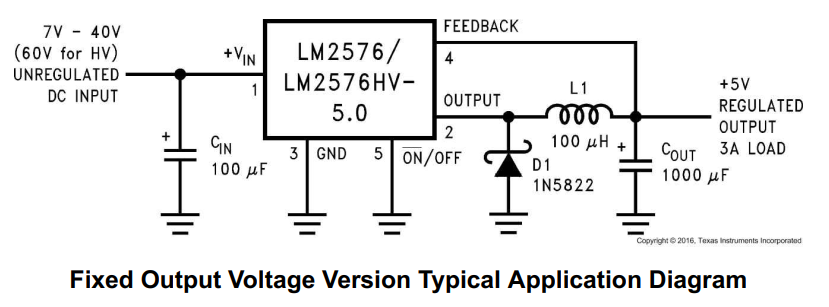
\includegraphics[width=13cm,keepaspectratio=true]{pics/buckConverter.png}
    \caption{Schaltplan des Buck Converters \autocite{buckConverter}}
    \label{buckConverter}
\end{figure}

Unter Last kommt es bei´der Benutzung des High-Power-Circuits zu hohe Spannungsabfällen von etwa 1 V.
Diese führen dazu, dass der Controller neu startet.
Die Verwendung der falschen Diode ist der wahrscheinlichste Grund für die starken Spannungsschwankungen unter Last.
Dieses Problem konnte bis zur Abgabe nicht behoben werden. \\
Ein weiteres Problem ist, dass die verwendeten Akkus lediglich eine dauerhafte Entladerate von 1 C haben, was bei 2000 mAh einen Strom von 2 A zu Folge hat.
Daher kann die Leistungsfähigkeit des LM2576 nicht ausgenutzt werden.\\
Die Benutzung der USB-Schnittstelle oder der Servos bei Verwendung des High Power Circuits führt daher zum Absturz.
Zur Abnahme wurden die Servos direkt an einen 2 s LiPo Akku angeschlossen.

\subsubsection{Akkuladegerät}\label{akkuCircuit}
\chapterauthor{Lukas Eigenstetter}
Das Akkuladegerät dient zum Laden von Akkus mithilfe der vom Solarpanel produzierten Energie.
Es orientiert sich an einem Blogpost zu einem Arduino-Ladegerät. \autocite{microfarat}
In diesem Kapitel werden die Schaltung und die Formeln zur Berechnung der Werte erklärt.\\
Der Strom wird am Haupt-ESP mithilfe eines PWM-Signals gesteuert.
Das Signal schaltet einen BC547 Bipolartransistor. \autocite{bipo}
Ist der Transistor auf Durchlass geschaltet, so wird der MOSFET, der den Ladestrom steuert, ausgeschaltet.
Als Leistungstransistor wurde ein IRF5305 im TO-220 Format verwendet. \autocite{irf}
Da die Batterie Schwingungen ausreichend dämpft, wurde keine zusätzliche Filterschaltung verbaut.
Vor den Akku wurde eine BY-255 Diode in Laufrichtung eingebaut, um Strom von der Batterie zu den Panelen zu verhindern.
Abbildung \autoref{charger} zeigt verbaute Schaltung. \\

\begin{figure}[htpb] % {H}
    \centering
    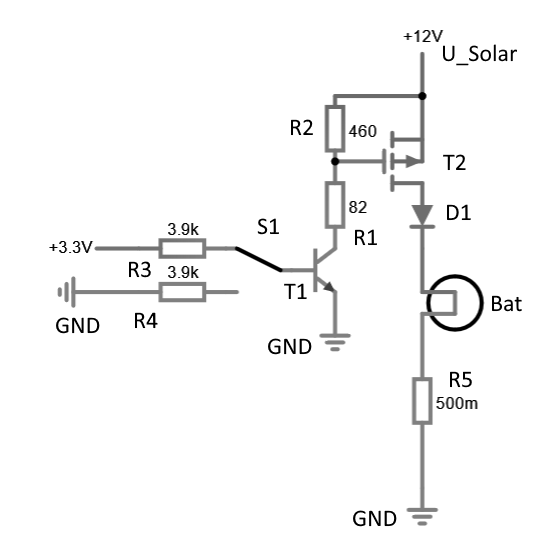
\includegraphics[width=9cm,keepaspectratio=true]{pics/charger.png}
    \caption{Schaltplan des Lade-PWM}
    \label{charger}
\end{figure}

Zusätzlich wurde Cell-Balancing realisiert.\\
Bei Lithium Polymer Akkus tritt das Problem auf, dass einzelne Zellen unterschiedlich schnell verschleißen.
Dann verliert eine Zelle schneller an Kapazität als die andere, wodurch die Verschlissene schneller ge- und entladen wird.
Die Zelle mit der geringeren Kapazität kann dann überladen oder zu tief entladen werden, wenn nur die Gesamtspannung gemessen wird.\\
In SunStorage wurde ein einfaches, passives Cell-Balancing umgesetzt. 
Es wird jeweils die Spannung der Zellen gemessen und miteinander verglichen.
Falls eine Zelle eine deutlich höhere Spannung als die Andere aufweist, wird sie über einen 82\textOmega \ Widerstand entladen, bis sich ein Gleichgewicht hergestellt hat. 
Dieses Verfahren wird auch als \emph{Current Bypass} bezeichnet. 
Die Spannungsdifferenz, ab der Balancing aktiviert wird, kann im Frontend eingestellt werden. \autocite[S. 111 - 127]{chargerBuch}\\
\begin{figure}[htpb] % {H}
    \centering
    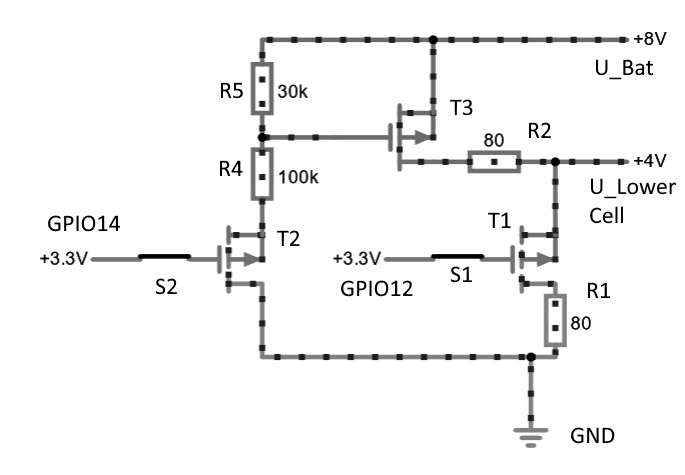
\includegraphics[width=15cm,keepaspectratio=true]{pics/balancing.png}
    \caption{Schaltplan Cell Balancing}\label{balancing}
\end{figure}

\autoref{balancing} zeigt die Schaltung, die das Cell-Balancing umsetzt.
Für die niedrigere Zelle wird der Transistor T1 Transistor direkt über GPIO12 geschaltet.
Da die obere Zelle auf +4 bis +8 Volt liegt und der PIN nur 3.3 Volt liefert, muss für die obere Zelle eine Schaltung mit zwei Transistoren verwendet werden.
T2 dient zur Herstellung der für den Schaltvorgang von T3 notwendigen Spannung.
Über T3 wird die obere Zelle entladen.
Da P-Kanal-Transistoren verwendet werden, ist die Logik der Schaltung negativ.
Sind die PINs beispielsweise HIGH, so fließt kein Strom.\\
Verbaut wurden IRLML2244 Transistoren im SMT Format. \autocite{irlml}
Um sie in ein Put-Through-Board zu integrieren, wurden sie zunächst an dickere PINs gelötet, die dann an das Board gelötet wurden.\\

Zur Messung der Spannungen und Ströme werden die ADC des Haupt-ESP verwendet.
Der Ladestrom kann über die an R8 abfallende Spannung gemessen werden.
Ist die Spannung positiv, so fließt Strom aus der Batterie in das System. Ist sie negativ, so wird mehr produziert als konsumiert und die Batterie wird geladen.
\autoref{messaufbau} zeigt den Teil des Systems, der für die Messungen relevant ist.
$I_{Solar}$ ist dabei der Strom des Panels und S1 symbolisiert das PWM Signal des Ladegeräts.
$R_{Sys}$ ist der Widerstand des Systems.
So wird der Stromverbrauch modelliert.
Aus Gründen der Übersichtlichkeit wurde auf die zwischen ADC- und GND geschalteten 100 nF Kondensatoren, die das Rauschen verringern, nicht eingezeichnet.
Der vollständige Schaltplan ist in \autoref{schaltplanHaupt} dargestellt.

\begin{figure}[htpb] % {H}
    \centering
    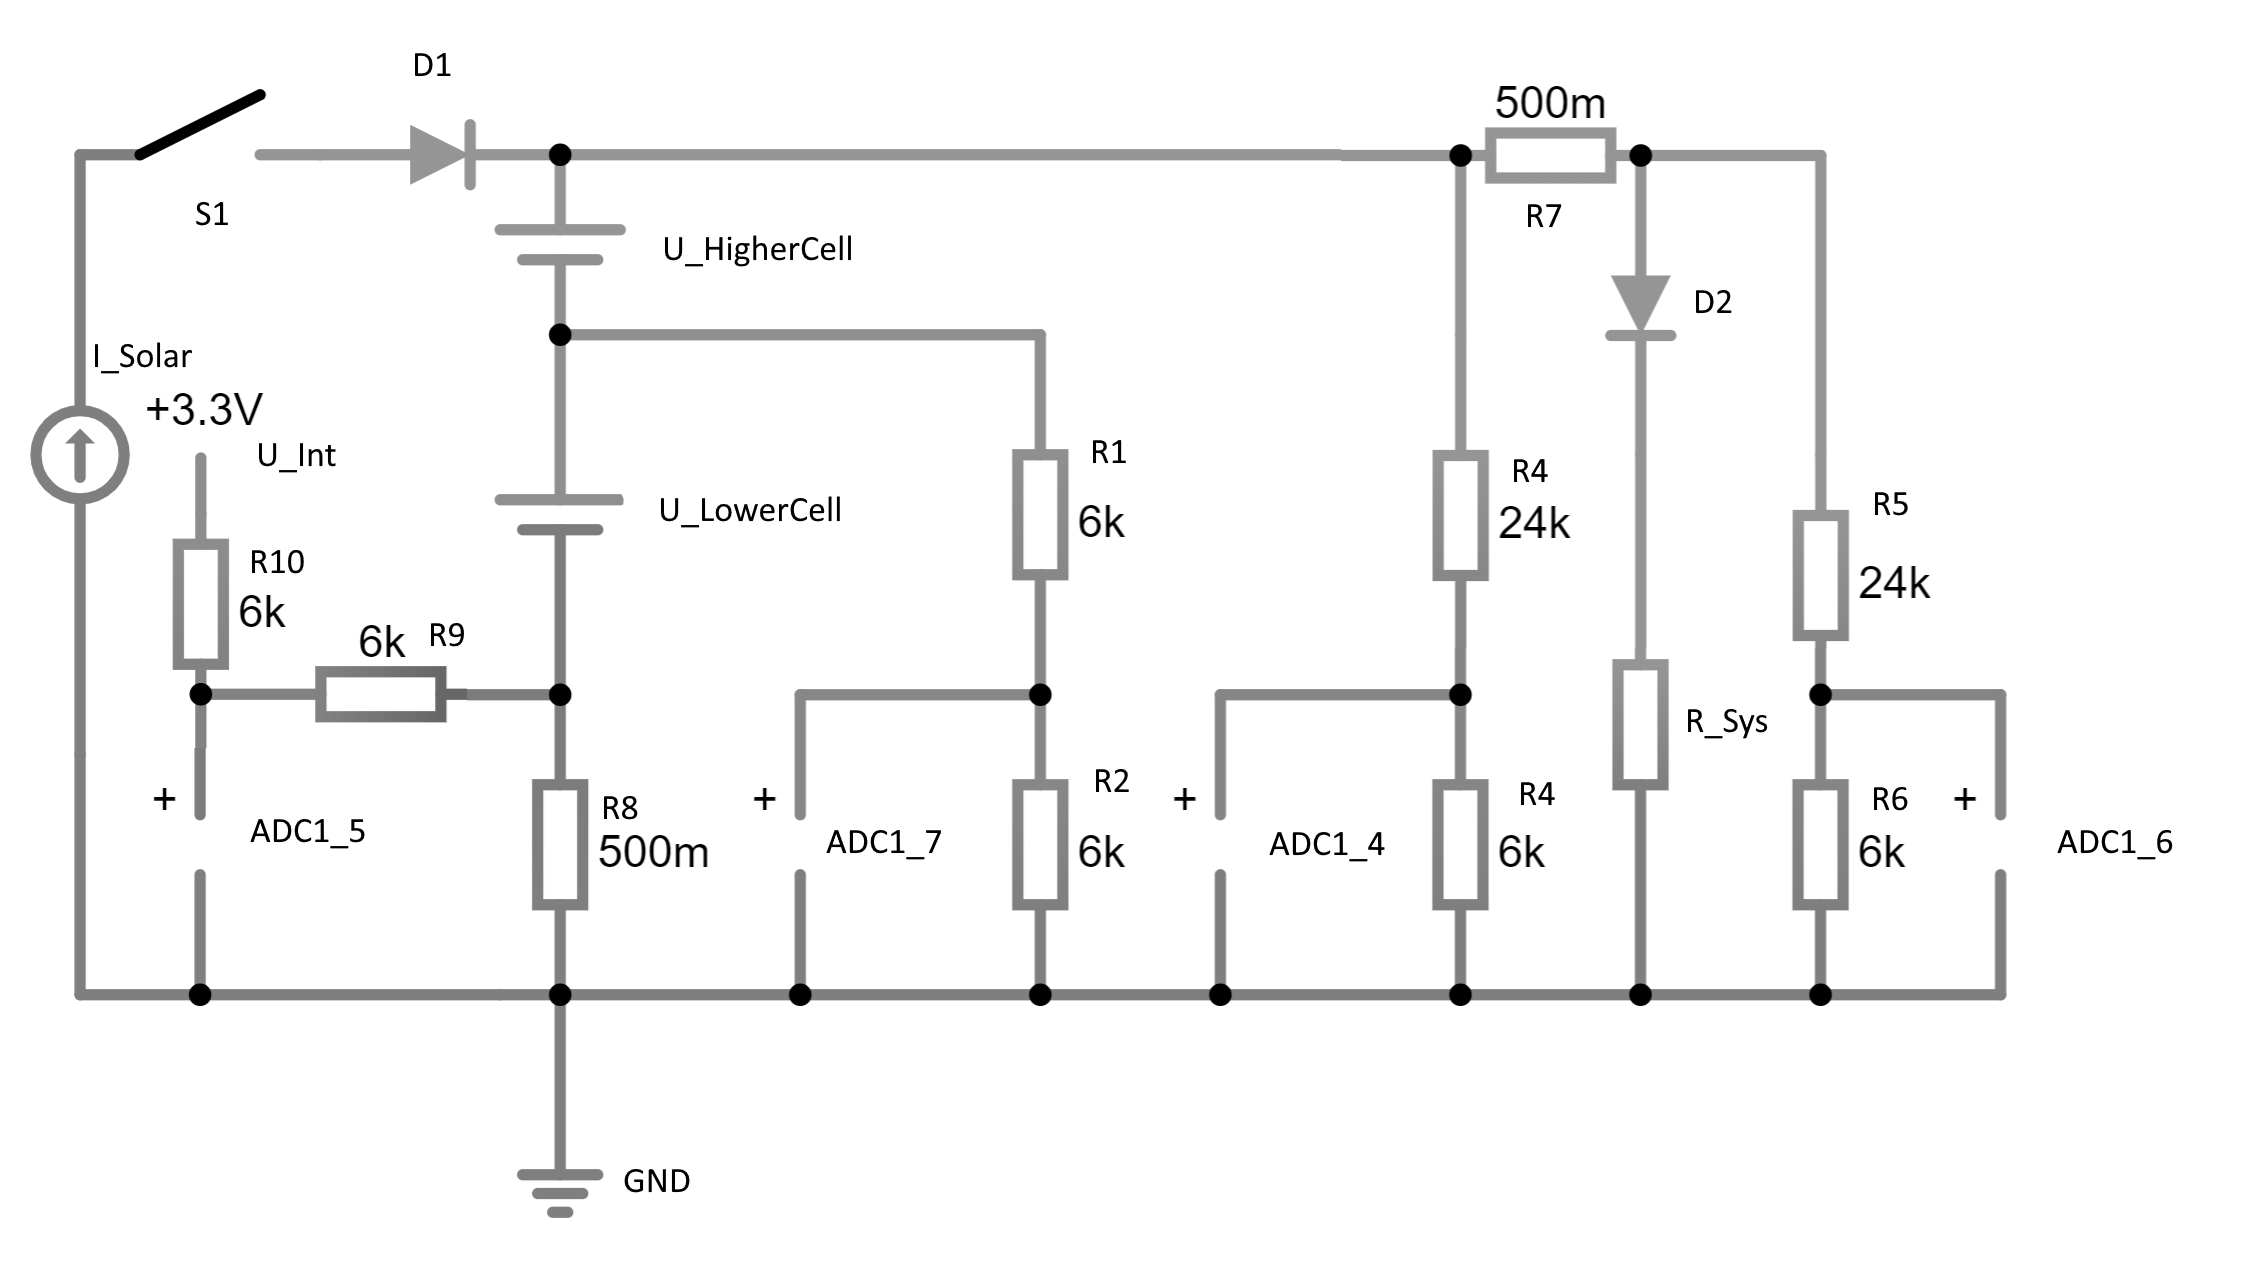
\includegraphics[width=16cm,keepaspectratio=true]{pics/measuring.png}
    \caption{Schaltplan des Messungsaufbau}
    \label{messaufbau}
\end{figure}

Da negative Spannungen nicht im Ansteuerbereich des ADC liegen, muss eine Pullupschaltung verwendet werden.
Mithilfe von R9 und R10 wird die Spannung am ADC auf 1.65 V gezogen.
Die tatsächlich am Widerstand anliegende Spannung muss daher um 1.65 V verringert werden:
$$ U_{ChargerShunt} = U_{0} - U_{ADC1\_5} $$
Der Ladestrom  ergibt sich durch die folgende Formel:
$$ I_{Charger} = I_{System} + U_{ChargerShunt} \cdot c_{SysSh}  $$

Die Konstanten können \autoref{adcCali} entnommen werden.
Die Spannung der niedrigeren Batteriezelle ergibt sich durch die Messung von ADC1\_7.
Um die Werte im Ansteuerbereich zu halten, wird ein Spannungsteiler aus R1 und R2 gebaut.
Zusätzlich muss die an R8 abfallende Spannung berücksichtigt werden.
Daraus ergibt sich die folgende Formel:
$$ U_{LowerCell} = (U_{ADC1\_7} + U_{ChargerShunt} \cdot \frac{c_{CharSh}}{c_{LC}}) \cdot c_{LC} $$
Für die Berechnung der Gesamtspannung wurde die selbe Schaltung verwendet.
Lediglich R4 muss erhöht werden, um den Spannungsbereich von ADC1\_4 zu erreichen.
Auch hier muss die Spannung an R8 berücksichtigt werden:
$$ U_{Battery} = (U_{ADC1\_4} + U_{ChargerShunt} \cdot \frac{c_{CharSh}}{c_{HC}}) \cdot c_{HC} $$
Mithilfe der Spannungen an ADC1\_6 und ADC1\_4 kann der Strom durch D2 und R\_Sys berechnet werden.
Die Diode wird in Laufrichtung betrieben und verhindert, dass Strom vom System in die Batterie fließt.
Dies könnte beispielsweise passieren, wenn ein PC zum Flashen oder Monitoring angeschlossen ist.
R\_Sys beschreibt vereinfacht den Widerstand des Systems.
Die Differenz aus der Spannung an ADC1\_4 und ADC1\_6 ist die an R7 abfallende Spannung und damit der Systemstrom.
Die konkrete Formel lautet:
$$ I_{System} = (U_{ADC1\_4} \cdot c_{HC} - U_{ADC1\_6} \cdot c_{SysDiv}) \cdot c_{SysSh} $$
Da die Widerstände nicht genau die Werte der Zeichnung besitzen, musste das Gesamtsystem kalibriert werden.
Dies wurde durch Messungen der Ströme und Spannungen mithilfe von Multimetern umgesetzt.
Da keine 6 k\textOmega \ Widerstände vorhanden waren, wurden 6.4 k\textOmega \ Widerstände verbaut. Diese weisen relativ hohe Abweichungen auf, weshalb die Kalibrierungswerte deutlich von den berechneten Werten abweichen.
Die Kalibrierungswerte des Endsystems lauten:

\begin{table}[H]
    \begin{center}
        \begin{tabular}{|l|l|l|r|}
            \hline
            Beschreibung                   & Symbol         & Variablenname                  & Wert \\
            \Xhline{3\arrayrulewidth}
            Pullup des Ladestroms          & $ U_{0} $      & VOLTAGE\_SOLAR\_0              & 1650 \\
            \hline
            Shunt für Ladestrom            & $ c_{SysSh} $  & SOLAR\_SHUNT\_TO\_AMPS         & 2.0  \\
            \hline
            Shunt für Verbrauch            & $ c_{CharSh} $ & SYSTEM\_SHUNT\_TO\_AMPS        & 2.0  \\
            \hline
            Spannung der niedrigeren Zelle & $ c_{LC} $     & VOLTAGE\_DIVIDER\_LOWER        & 2.26 \\
            \hline
            Spannung der Batterie          & $ c_{HC} $     & VOLTAGE\_DIVIDER\_BATTERY      & 4.05 \\
            \hline
            Spannung Verbrauchsmessung     & $ c_{SysDiv} $ & VOLTAGE\_DIVIDER\_SYS\_CURRENT & 3.65 \\
            \hline
        \end{tabular}
        \caption{Kalibrierung der ADC Berechnungsparameter}
        \label{adcCali}
    \end{center}
\end{table}

Zum Auslesen der ADC wird die ADC-Oneshot-API der Espressif IDF verwendet.
Da die ADC Messwerte Ausschläge von bis zu 30 mV aufweisen, wird ein gleitender Mittelwert aus den letzten Messungen gebildet.
Dafür werden zu jedem Zeitpunkt die letzten zehn Werte betrachtet, wobei der Höchste und der Niedrigste verworfen werden.
Aus den restlichen acht Werten wird der Mittelwert gebildet.
Durch die Mittelwertbildung können die Schwankungen der Messungen ausgeglichen werden.
Aufgrund der gleichzeitigen Nutzung des WiFi konnten nur PINs des ADC1 verwendet werden.\\
Die zehn letzten Werte liegen im Programm in einem Ringbuffer vor.
Um das Minimum und das Maximum zu bestimmen, wird dieser kopiert und die Kopie wird sortiert.
Alle Berechnungen werden mit Fixkommazahlen im Milli-Bereich durchgeführt.\\
Problematisch an dieser Vorgehensweise ist zum einen, dass kurze Spannungspitzen möglicherweise nicht registriert werden.
Außerdem wirken sich Veränderungen der Messwerte erst mit einer gewissen Verzögerung erkennbar auf den Ergebniswert aus.
Diesen Effekten wird durch eine Erhöhung der Abtastrate von 1 Hz auf 10 Hz entgegengewirkt.

Die in diesem Kapitel erklärten Berechnungen sind in der Simulation korrekt.
In \autoref{fig:graphen} ist erkennbar, dass die tatsächlich gemessenen Werte falsch sind.
Zum einen sind die Ströme zu hoch.
Dies führt dazu, dass unter Last auch die Spannungsmessungen verfälscht werden.
Der genaue Grund konnte bis zum Ende des Projekts nicht gefunden werden.
Es könnte entweder an einem nicht berücksichtigten Faktor und damit einem Fehler in der Simulation und Modellierung liegen.
Eine weitere Möglichkeit ist ein Fehler in der Umsetzung des Schaltkreises.

\subsubsection{USB-Schnittstelle}\label{usbSchnittstelle}
\chapterauthor{Lukas Eigenstetter}
Die USB Schnittstelle wird durch den High-Power-Circuit (\autoref{HPC}) versorgt.
Die grundlegenden Lademodi in den meisten Handys werden durch das Anlegen einer bestimmten Spannung an den mittleren PINs des USB Ports festgelegt.
Für höhere Ladeströme gibt es spezielle Protokolle wie beispielsweise \emph{Quick Charge}. \autocite{quickCharge}
\autoref{UsbModi} zeigt die umgesetzten Modi und die verwendeten Schwellspannugen.

\begin{table}[H]
    \begin{center}
        \begin{tabular}{|l|r|r|}
            \hline
            Modus          & PIN 1 & PIN 2 \\
            \Xhline{3\arrayrulewidth}
            500 mA (2.5 W) & 2.0 V & 2.0 V \\
            \hline
            1 A (5 W)      & 2 V   & 2.8 V \\
            \hline
            2,1 A (10 W)   & 2.8 V & 2.0 V \\
            \hline
        \end{tabular}
        \caption{Spannung an mittleren PINs in für den jeweiligen Lademodus. PIN 1 ist neben GND. \autocite{usbProtokoll}}
        \label{UsbModi}
    \end{center}
\end{table}

Je nach Modus werden die DAC Pins auf die passende Spannung gesetzt.
Der Buck-Converter kann laut Datenblatt dauerhaft einen Strom von 3 A liefern.
Damit ist der Stromkreis auch im 10 W Modus hinreichend versorgt.

\subsubsection{Coulomb-Counter}
\chapterauthor{Matthias Unterrainer}
\begin{figure}[htpb]
    \centering
    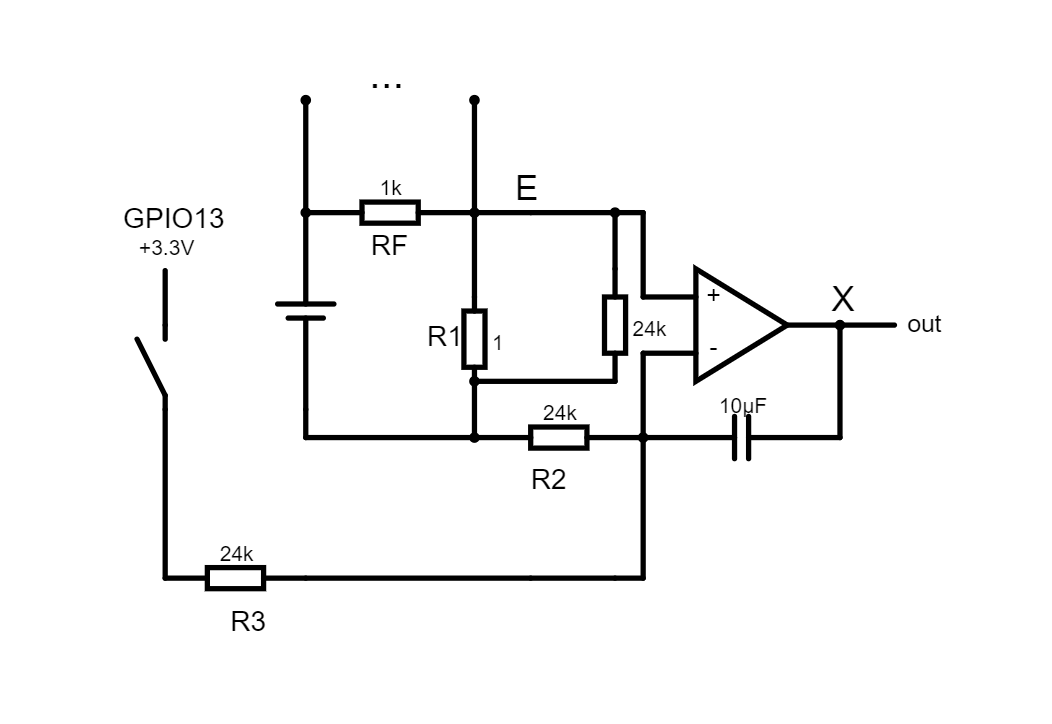
\includegraphics[width=0.7\linewidth,keepaspectratio=true]{pics/coulomb_counter_circuit.png}
    \caption{Schaltplan des Coulomb-Counters}
    \label{fig:coulomb_counter}
\end{figure}

Um effektiv den Stromfluss im Schaltkreis messen zu können, wurde ein Coulomb-Counter entworfen und eingebaut.
Ein Coulomb-Counter funktioniert im Pinzip so, dass ein bestimmter Strom durch einen Stromkreis fließt, dieser kann denn Akku laden oder entladen. Wenn jetzt die Ladung im Akku zu Beginn der Messung bekannt ist, dann kann allein durch das Wissen, wie viel Ladung ge-/entladen wurde, relativ genau bestimmt werden, wie viel Ladung im Akku noch übrig ist. Dazu wird der Strom mithilfe eines sehr kleinen Widerstandes $R_1$, unter dem ohmschen Gesetz $R = \frac{U}{I}$, welches die Beziehung zwischen Strom und Spannung beschreibt, in eine Spannung ''umgewandelt''. Da hier für $R_1$ ein Widerstand von 1 Ohm gewählt wurde, entspricht der Strom der durch den Widerstand fließt der über den Widerstand anliegenden Spannung. Da der Coulomb-Counter jedoch für Ströme bis zu 2 A ausgelegt sein sollte, was zu einer Spannung von 2 V führen würde, musste diese, aufgrund der Funktionsweise des Op-Amps, noch durch einen Spannnungsteiler reduziert werden. Hierbei wurde die Eingangsspannung durch den Spannungsteiler der sich aus $R_F$ und $R_1$ zusammen setzt, wobei $R_F$ 1 k$\Omega$ ist, auf ca. $\frac{1}{1000}$ der Eingangsspannung reduziert. Genauer auf $V_{\text{in}} \cdot \frac{1 \Omega}{1000 \Omega + 1 \Omega} = 0.\overline{000999} \cdot V_{\text{in}}$. Dadurch wird die maximale Eingangsspannung bei einer maximal Last von 2 A auf 2 mV begrenzt.\\\\
Dies ist jedoch erst der erste Schritt, da bis jetzt nur eine Spannung äquivalent zu ca. $\frac{1}{1000}$ der Eingangsspannung an der Stelle $E$ gemessen werden kann. Dies beschreibt lediglich den aktuellen Strom, der in diesem Moment durch den Stromkreis fließt, enthält aber noch keine Informationen über die zeitliche Komponente, also darüber, wie viel Strom in einer bestimmten Zeit durch den Stromkreis geflossen ist. Um diese aussagekräftigere Messung aus den einzelnen Momentanaufnahmen zu erhalten, müssen diese über die Zeit integriert werden. Dies wird mithilfe eines analogen Integrators bewerkstelligt. Dieser setzt sich aus einem Operationsverstärker (Op-Amp), dem LMC6462 Op-Amp, und einem 10 $\mu$F Kondensator zusammen.\\\\
\begin{figure}[htpb]
    \centering
    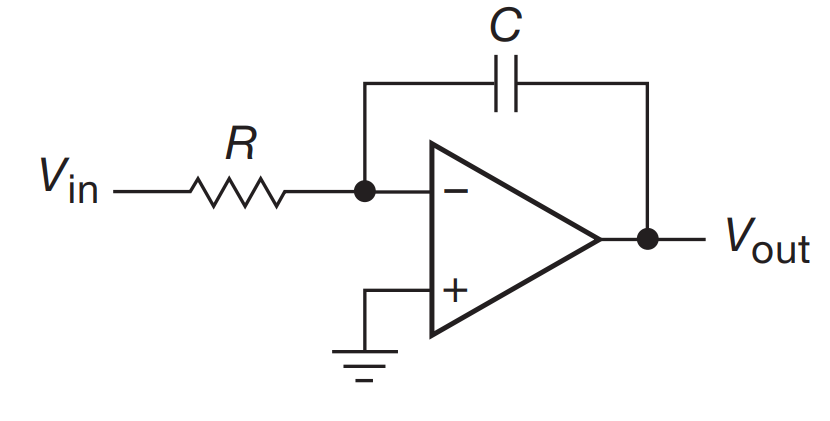
\includegraphics[width=0.5\linewidth,keepaspectratio=true]{pics/analog_integrator.png}
    \caption{Grundlegender Aufbau eines Op-Amp Integrators. \cite{aoe}}
    \label{fig:analog_integrator}    
\end{figure}
Abb. \ref{fig:analog_integrator} zeigt den Aufbau eines Op-Amp Integrators. Der Eingangsstrom $\frac{V_{\text{in}}}{R}$ fließt durch den Kondensator $C$, und da der invertierende Eingang ein virtueller Nullpunkt ist, wird die Ausgangsspannung durch
$$V_{\text{out}}(t) = - \frac{1}{RC} \int V_{\text{in}}(t) dt + \text{ const.}$$
gegeben. Daraus folgt
$$\Delta V_{\text{out}} = - \frac{V_{\text{in}}}{RC} \Delta t = - \frac{I_{\text{in}}}{C} \Delta t$$ \cite{aoe}

\begin{figure}[htpb]
    \centering
    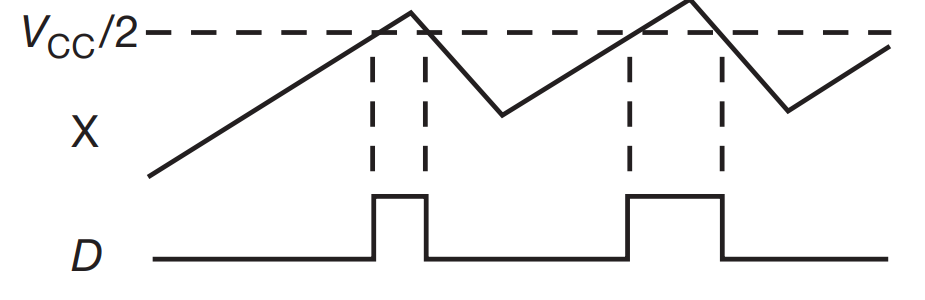
\includegraphics[width=0.5\linewidth,keepaspectratio=true]{pics/coulomb_counter_output.png}
    \caption{$X$ ist der Output des Integrators, $V_{CC}$ ist hier 3.3 V und $D$ ist der resultierende Duty-Cycle. \cite{aoe}}
    \label{fig:coulomb_counter_output}    
\end{figure}

In Abb. \ref{fig:coulomb_counter_output} ist der Output des Integrators ($X$) zu sehen. Dieser wird mit einer festen Spannung (hier $\frac{V_{CC}}{2}$, was aber für die entgültige Rechnung unwichtig ist) verglichen und aus der Zeit die $X$ größer als die Vergleichsspannung ist, wird ein Duty-Cycle $D$ abgeleitet. Da solange keine negative Spannung anliegt das Integral immer weiter steigt (zumindestens bis zur Obergrenze $V^+$), muss, wie in Abb. \ref{fig:coulomb_counter} zu sehen, der Integrator regelmäßig ''entladen'' werden. Dies geschiet via einer ''Entladespannung'', die hier über den GPIO-Pin 13 angelegt wird. Da wie bereits erwähnt der Output proportional zu $I_{in}$ bzw. $\frac{I_{in}}{C}$ steigt und proportional zu der ''Entladespannung'' $\frac{V_{CC}}{R_{3}} - \frac{I_{in}}{C}$ fällt, kann daraus die Länge des Duty-Cycles ermittelt werden. Da in diesem Entwurf, wenn der GPIO-Pin13 auf GND gezogen ist, $R_3$ und $R_2$ in parallel zu einander geschalten sind, entspricht der Widerstand beim ''Laden'' $R_{cha} = \frac{R_2 R_3}{R_2 + R_3} = \frac{24k\Omega \cdot 24k\Omega}{24k\Omega + 24k\Omega} = 12k\Omega$.  Daraus folgt, dass der Duty-Cycle $D$ über längere Zeit
$$D = \frac{I_{in} R_{3}}{C V_{CC}} \Rightarrow I_{in} = \frac{D \cdot C \cdot V_{CC}}{R_{3}}$$\cite{aoe}\\\\
Somit repräsentiert $I_{in}$ den Strom der durch das System seit Messbeginn geflossen ist.\\\\
Der LMC6462 Op-Amp wurde gewählt, da dieser einen kleinen Input Offset Voltage von nur 0.25 mV hat. Dies entspricht einem maximalen Offset Fehler von $e_{\text{off}} = \frac{V_{os}}{V_{in,max}} = \frac{250 \mu V}{2 V} = \frac{1}{8000}$ dies entspricht einem Messfehler von 25 mA ($2 A \cdot \frac{1}{8000} = 2.5 \times 10^-4$A) bzw. einer Auflösung von 8000:1. Und da dieser eine sehr niedrige Versorgung von nur 20$\mu$A / Amplifier benötigt.
Ein weiterer Grund für den LMC6462 war sein Rail-to-Rail Output mit einem maximalen Offset von diesem von unter 10 mV, da dadurch bei einem $V^+$ von 3.3 V der Output des Integrators nie 3.4 V überschreitet und somit den ADC Pin, der bis zu 3.9 V messen kann, nie überlasten wird. \cite{LMC6462_data_sheet} Und es wurde eine 10 $\mu$ F Kondensator gewählt, da der Coulomb-Counter Output mit 10Hz abgetastet wird, ergibt sich dass mit $R_3 = 12k\Omega, f = 10Hz, C = 10 \mu F$, dass der Integrator nie mit mehr als $C \cdot f \cdot R_3 = 10 \mu F \cdot 10Hz \cdot 12000 \Omega = 1.2$ also $\frac{V_{CC}}{1.2}$ pro Taktzyklus steigt oder fällt. \cite{aoe}

\paragraph{Probleme}
\chapterauthor{Matthias Unterrainer}
Das Hauptproblem mit dem Coulomb-Counter ist, dass zum einem der Input Rail-to-Rail ist, aber $V^- =$ GND und $V^+ = 3.3$ V ist. Dadurch kann generell keine negative Spannung, die beispielsweise beim Lade auftreten könnte, im Integral berücksichtigt werden, wodurch der Coulomb-Counter nur die Entladung richtig misst. Da aber das ganze Konzept von Coulomb-Counting darauf beruht, dass man genau darüber bescheid weiß, wie viel Ladung in den Akku rein- oder rausgeflossen ist, zerstört dies jeden Ansatz einer akuraten Messung.\\
Dies ist zwar generell ein Problem, aber in diesem Aufbau vernachlässigbar, da der Coulomb-Counter so eingebaut wurde, dass die zu messenden Spannung $V_{in} < 1.65 V$ beim Laden und $V_{in} > 1.65 V$ beim Entladen beträgt. Dieser Aufbau führt allerdings zu deutlich erheblicheren Problemen, da erstens, dass Integral dadurch von den Werten her verschoben wird, was zwar noch nachträglich lösbar ist, aber das Hauptproblem ist der zweite Punkt, dass dadurch vor allem beim Laden sehr kleine Spannungen anliegen. Dies ist ein Problem, da wie oben bereits erwähnt, der Coulomb-Counter auf 2 A ausgelegt wurde unde deshalb extra ein Spannungsteiler eingebaut wurde, um die ''Startspannung'' niedrig zu halten, damit eine akurate Messung möglich ist. Wenn jedoch nur eine Spannung von 0.1 V anliegt, was einer relative hohe Ladespannung entsprechen würde, dann liegen Aufgrund des Spannungsteilers nur etwa 0.1 mV am Op-Amp an. Es folgt daraus, dass um die Vergleichsspannung von 1.65 V zu erreichen, mit $\Delta V_{\text{out}} = - \frac{V_{\text{in}}}{R_{chr}C} \Delta t \Rightarrow \Delta t = \frac{\Delta V_{out} \cdot R_{chr} \cdot C}{V_{in}} = \frac{1.65 V \cdot 12 k\Omega \cdot 10 \mu F}{0.1 mV} = 1980 s = 33 min$. Es würde also über eine halbe Stunde dauern, um nur eine Spitze des Duty-Cycles zu erreichen, was ein großes Problem ist, da das ganze Konzept auf vielen kleinen Messungen basiert, welche zwar einzeln gesehen teilweise größere Abweichungen haben, aber in der Summe ein relativ gutes Gesammtbild schaffen.

\subsubsection{Realisierung}
\chapterauthor{Lukas Eigenstetter}
In diesem Kapitel wird die konkrete Realisierung der Schaltung beschrieben.
Dabei werden die Probleme und angewendeten Techniken beschrieben.\\

\paragraph{Haupt-ESP}
\chapterauthor{Lukas Eigenstetter}
Das Ladegerät und der Haupt-ESP sind auf einer 40 x 40 Put-Through Platine verlötet.
Diese besitzt durchgezogene Leiterbahnen auf der Unterseite.
Mithilfe eines Dremel-Schleifers wurden diese an bestimmten Stellen durchtrennt, um die gesamte Schaltung auf diesem Board unterzubringen.\\
\autoref{schaltplanHaupt} zeigt den Schaltplan.
Für Ein- und Ausgänge wurden jeweils PINs verlötet, die eine Verbindung mit Jumper-Kabeln erlauben.
Aus Platzmangel mussten am tatsächlichen ESP auch Leitungen zwischen Controller und Platine verbaut werden.
Diese sind in der Zeichnung direkt oberhalb des Controllers eingezeichnet.
Widerstände, die in Reihe geschaltet sind, und Draht der zur Verlängerung der Verbindungen einiger Bauelemente benötigt wurde, sind oberhalb der Platine verbunden.
Dies wurde durch Verdrillen und Verlöten gelöst.\\
Zusätzlich befindet sich auf dieser Platine die Stromversorgung und der Buck-Converter.
Um den Kapazität für das Filter des Abwärtswandlers zu realisieren, mussten sechs Kondensatoren parallel geschaltet werden.
Auch hier wurde das Verfahren des Verdrillens und Verlötens angewendet.
Um die Schaltung noch kompakter zu gestalten wurden die 1 \textOmega \ / 3 W Leistungswiderstände teilweise vertikal verbaut.

\begin{figure}[htpb] % {H}
    \begin{center}
        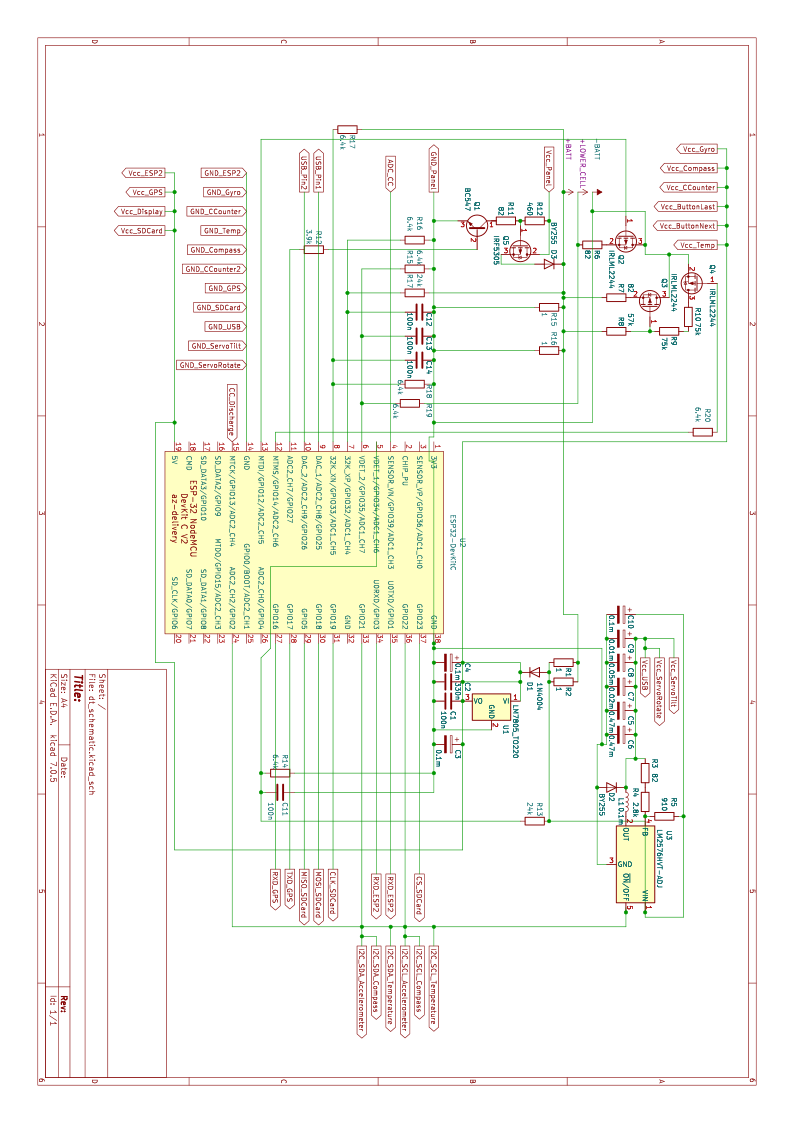
\includegraphics[width=15cm,keepaspectratio=true]{pics/hauptespSchaltung_svg-raw.png}
        \caption{Schaltplan des Hauptcontrollers}
        \label{schaltplanHaupt}
    \end{center}
    Im Dokumentationsordner liegen ein SVG und die KiCad Datei zur besseren Lesbarkeit und Nachvollziehbarkeit bei.
\end{figure}
\clearpage


\paragraph{Neben-ESP}
\chapterauthor{Matthias Unterrainer}
Der Neben-Esp wird nur verwendet um die Servos und das LCD Display zu steueren. Dazu werden die notwendigen Daten via UART vom Haupt-Esp an den Neben-Esp geschickt.
\begin{figure}[htpb] % {H}
    \begin{center}
        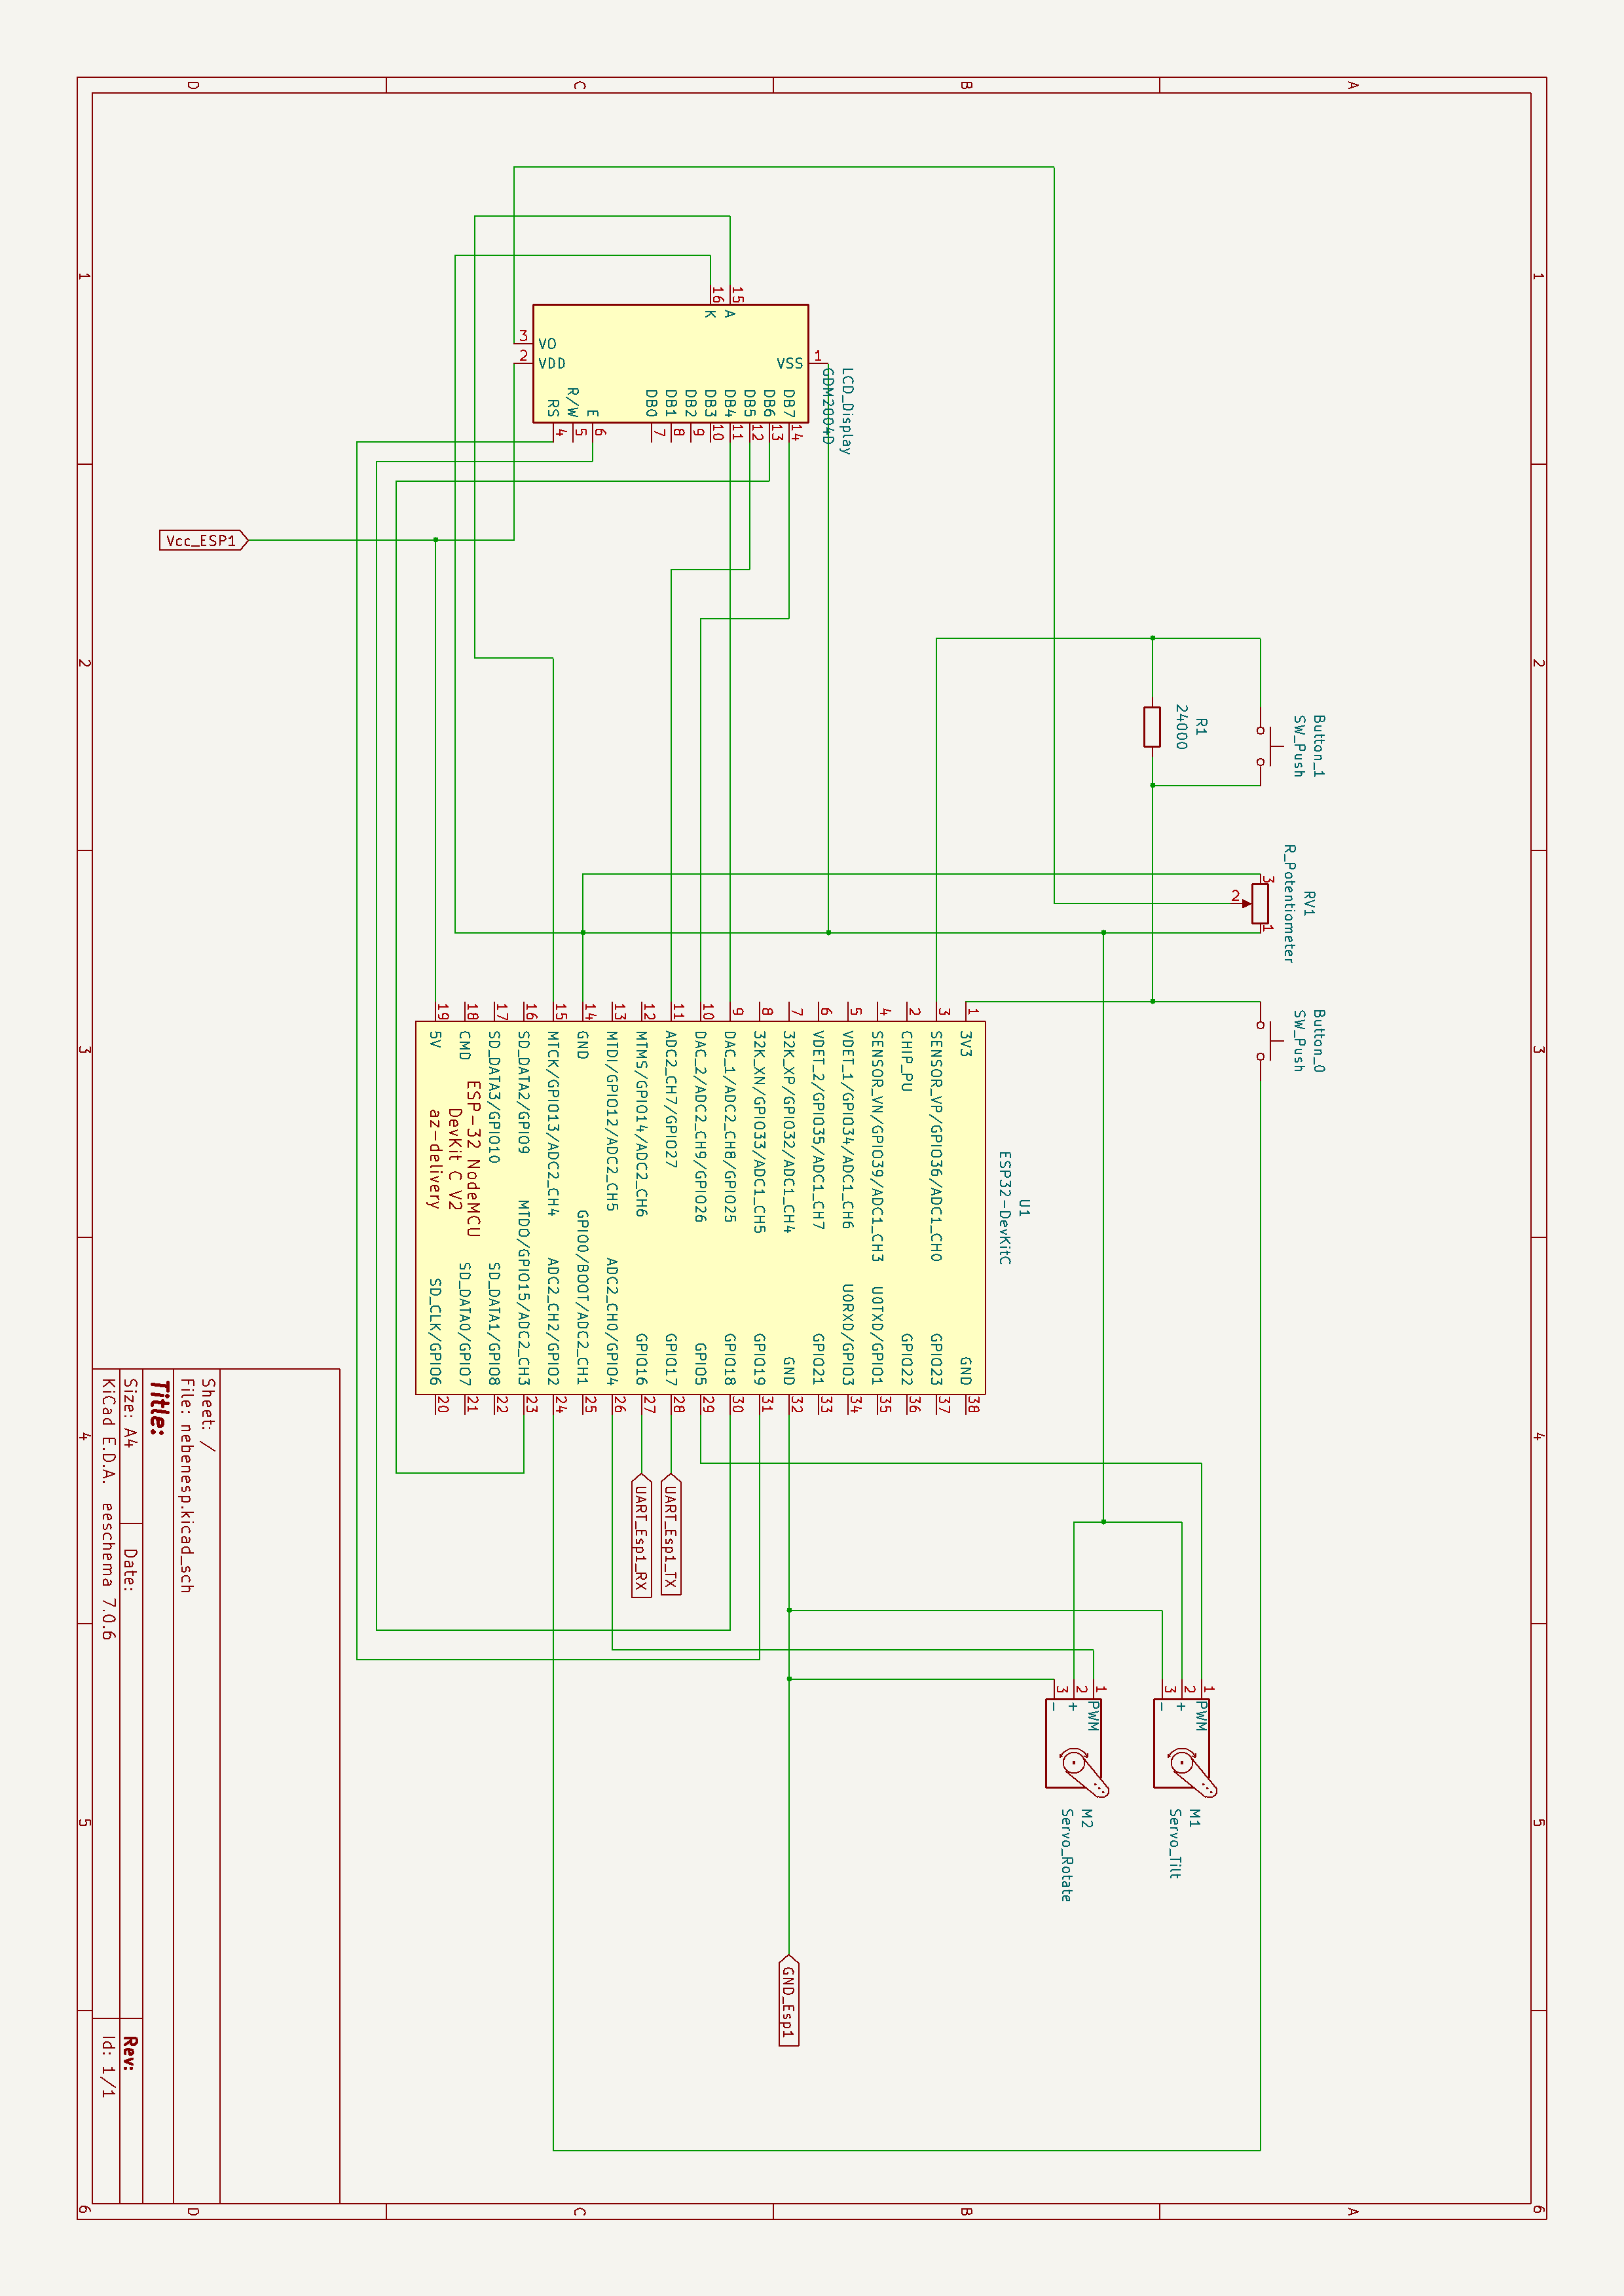
\includegraphics[width=15cm,keepaspectratio=true]{pics/circuit_nebenesp.png}
        \caption{Schaltplan des Nebenesps}
        \label{curcit_nebenesp}
    \end{center}
    Im Dokumentationsordner liegen ein SVG und die KiCad Datei zur besseren Lesbarkeit und Nachvollziehbarkeit bei.
\end{figure}

\subsection{Datenverwaltung}
\chapterauthor{Philipp Thaler}
Das Projekt SunStorage hat verschiedene Systemzustände und muss auch historische Daten speichern können. Zudem kann auch die WLAN Konfiguration bearbeitet werden.
Um diese Funktionen bereitzustellen ist es nötig, dass das System über eine Datenverwaltung verfügt.

Die folgenden Kapitel geben einen detailierten Einblick, wie das System intern Daten speichert und verwendet.

\subsubsection{SPI Flash File System}
\chapterauthor{Philipp Thaler}
Das Serial Peripheral Interface Flash File System (SPIFFS) ist ein einfaches Dateisystem, welches für Mikrokontroller mit einem SPI Flash Chip geeignet ist. Das verwendete ESP-32 Board von AZ-Delivery stellt insgesamt 4MB Speicherplatz zur Verfügung.
SPIFFS unterstützt das Wear-Leveling. Dies dient dazu, dass die Lebensdauer für Flash-Speicher oder anderer ähnlich aufgebauten Speicherarchitekturen verlängert wird.

Eine Eigenheit des Dateisystems ist, wie es mit Ordnerstrukturen umgeht. Erstellt man eine Datei in einem Ordner, so wird kein Ordner erstellt wie man es von Windows oder Linux kennt. Es wird eine Datei erstellt, die mit dem Namen des Ordners versehen wird.
Zum Beispiel erstellt man eine Datei im Ordner Frontend, dann wird die Datei \glqq /Frontend/index.html\grqq{} im SPIFFS genannt.
Dadurch weiß das Dateisystem, wenn der Benutzer über den vermeintlichen Ordner Frontend auf die index.html Datei zugreifen möchte, welche Datei es ansprechen muss.
Auch gibt es Probleme beim Löschen einer Datei. Hier kann es dazu kommen, dass SPIFFS die Datei nicht vollständig löscht und es zu nicht mehr nutzbaren Sektoren im Speicher kommt.

Im Projekt wird das SPI-Dateisystem genutzt, um die Dateien der Webseite zu speichern. Zunächst wird dazu eine Datei mit den definierten Partitionen erstellt, die \glqq partitions.csv\grqq{} heißt. Diese gibt dem Dateisystem vor, wie viel Speicher welcher Partition zugewiesen wird.
Da das SPIFFS nur etwa 75\% des angegebenen Speichers belegen kann, ist der Speicher etwas großzügiger vergeben. In der \glqq partitions.csv\grqq{} sind die Partitionen aufgelistet die erstellt werden, sobald das Dateisystem gebaut wird \autocite{espidf:SPIFFS}.

Die Partitionstabelle wird mit dem Offset 0x8000 in den Flash geschrieben. Jeder Eintrag in der Partitionstabelle hat einen Namen, Typ, Untertyp und einen Offset ab dem er in den Flash geschrieben wird.
In diesem Fall sind keine Offsets vergeben. Hier entscheidet das Dateisystem selbst an welche Stelle die Partition geschrieben wird.

Zunächst wird für den Non-volatile Storage (nvs) eine Partition erstellt. Diese ist sechs Kilobyte groß. Hier können Key Value Paare gespeichert werden.
Unter dem Namen \glqq phy\_init\grqq{} wird die physikalische Sicht initialisiert. Diese wird genutzt um generelle Netzwerktätigkeiten verfügbar zu machen. Die Größe hier beträgt vier Kilobyte.

Als Vorletztes wird die Applikation definiert. Diese wird mit dem Kürzel  \glqq factory\grqq{} in der Partitionstabelle aufgeführt. Die dort abgelegten Dateien werden beim Start des ESP32 vom Bootloader ausgeführt. Die Größe dieser Partition beträgt ein Megabyte.
Den größten Platz mit zwei Megabyte wird SPIFFS zugewiesen. Hier werden die Dateien, die aus dem Buildprozess der Webseite erstellt werden, abgelegt. Da ReactJS sehr große Build-Artefake erzeugt, ist es notwendig die Partition am größten zu wählen.

Um das Dateisystem zu erstellen wird die Visual Studio Code Erweiterung PlatfromIO verwendet. In der \glqq platformio.ini\grqq{} Datei wird die \glqq partitions.csv\grqq{} als neue Partitionstabelle hinterlegt.
Somit kann PlatformIO die Partitionen direkt ableiten und entsprechend erstellen.
Damit der Compiler, in diesem Fall CMake, weiß welche externen Dateien zum Bauen des Dateisystems verwendet werden sollen, wird in der CMakeLists.txt im src-Ordner ein Befehl eingefügt.
Der Befehl gibt an, dass aus dem \glqq data\grqq{} Ordner die statischen Dateien der Webseite verwendet werden sollen.
Nach dem erfolgreichen Erstellen des Dateisystems, wird es mit Hilfe von PlatformIO auf die ESP32 Platine geladen.

Die Inizialisierungsfunktion für SPIFFS wird aus der app\_main-Funktion aufgerufen. Es wird eine spiffsConfig erstellt. Diese beinhaltet den Pfad unter dem das Dateisystem bereitgestellt wird. Die Partitionsbezeichnung und auch die maximale Anzahl an Dateien wird der Konfiguration übergeben.
Wenn benötigt, kann hier eingestellt werden, dass das Dateisystem formatiert wird sollte das mounten nicht ordnungsgemäß ausgeführt werden.

Nach dem Erstellen der Konfiguration wird diese dem Registrierungsbefehl übergeben. Dieser wird von dem ESP-IDF Framework bereitgestellt. Es folgen Fehlerüberprüfungen und eine Überprüfung wie viel Speicher bereits belegt ist und wie viel Speicher noch verfügbar ist.
Nach der erfolgreichen Ausführung stehen die Dateien dem System bereit und können gelesen und bearbeitet werden.



\subsubsection{CSV-Historie}\label{csvhistory}
\chapterauthor{Johannes Treske}
Eine Historie der Messdaten wird benötigt, um eine grafische Darstellung über die Zeit, im Web-Frontend darzustellen.
Ursprünglich war geplant, eine SQLite Datenbank zu verwenden.
Diese sollte auf der SD-Karte gespeichert werden.
Es gibt jedoch nur SQLite Bibliotheken, die mit älteren Versionen von ESP-IDF kompatibel sind, welche aber von unserem Modell des ESP32 nicht unterstützt werden.
Deswegen nutzen wir CSV-Dateien zum Speichern der Messdaten.

Für jeden Tag wird eine eigene CSV-Datei verwendet, die nach einem Teil des Timestamps benannt wird (YYYYMMDD.csv).
Innerhalb einer Datei besteht eine Zeile immer aus einer Reihe an Messdaten, eindeutig bestimmbar durch den Timestamp und getrennt durch Kommas.
Eine Zeile besteht aus allen Messwerten, die im Datenbankmodell in \autoref{fig. Datenbankmodell} zu sehen sind.
Um eine einfache Interaktion mit der Datenbank zu ermöglichen, wurde das Datenbankinterface geschrieben.
Die zwei wichtigsten Funktionen ermöglichen das Schreiben eines Messdatensets bzw. das Auslesen von Messdaten.

\begin{lstlisting}[language=C]
esp_err_t dbStoreReadings(readings_data_set_t readings);
esp_err_t dbGetReadings(readings_read_config_t config, cJSON** jsonOut);
\end{lstlisting}

Die Funktionsdeklaration der Lese-Funktion zeigt, dass ein JSON-Objekt zurückgegeben wird.
Dieses Objekt besteht aus einem JSON-Array, der alle Messdaten der gewünschten Zeitspanne, in Sets zusammengefasst, enthält.
Das JSON-Objekt kann so direkt an das Web-Frontend weitergegeben werden.
Über den \textit{config} Parameter kann eingestellt werden, welcher Zeitbereich abgefragt werden soll und welche Spalten/Messdaten benötigt werden.

Bei allen Funktionen des Datenbankinterfaces muss stets darauf geachtet werden, dass nicht mehrere Tasks auf die gleiche Datei zugreifen können.
Dieses Problem wird durch das Verwenden von Mutexen gelöst.
Weitere Funktionen, die das Datenbankinterface bereitstellt, sind Funktionen zum Initialisieren bzw. Deinitialisieren, sowie Funktionen, mit denen Daten gelöscht werden können.

\begin{figure}
    \centering
    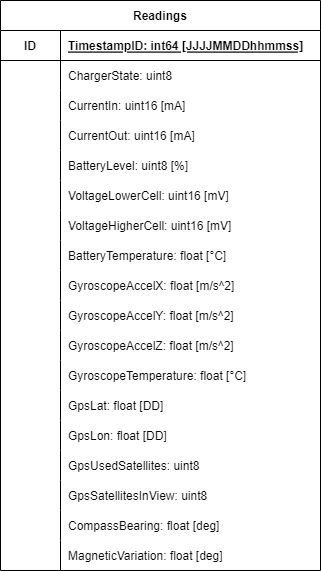
\includegraphics[width=0.5\textwidth]{pics/datenbankmodell.png}
    \caption{Datenbankmodell}
    \label{fig. Datenbankmodell}
\end{figure}


\subsubsection{Systemzustand}\label{Systemzustand}
\chapterauthor{Lukas Eigenstetter}
Der Systemzustand beschreibt alle Werte, die zwischen Neustarts des Systems erhalten bleiben sollen, für die keine Historie benötigt wird.
So können Konfigurationswerte aus dem Frontend erhalten bleiben.
Weitere Zustandsinformationen umfassen zuletzt gelesene Sensorwerte oder Stellwerte der Servos.\\
Der Zustand wird durch ein JSON-Objekt realisiert, das die Daten als Singleton hält und einen synchronisierten Austausch ermöglicht.
Beim Systemstart wird versucht, die Datei \textbf{state.txt} auf der SD-Card zu lesen und als JSON zu parsen.
Falls die Datei einige Werte nicht enthält oder fehlt, werden Defaultwerte verwendet.\\
Im Betrieb wird der Zustand alle 5 Sekunden geschrieben.
\autoref{tableStateCharger} zeigt alle Werte mit Bezug zum Ladegerät, die im finalen Zustandsobjekt enthalten sind.\\
\begin{table}[H]
    \begin{center}
        \begin{tabular}{|l|l|}
            \hline
            Name                  & Beschreibung                                           \\
            \Xhline{3\arrayrulewidth}
            usbMode               & Modus der USB-Schnittstelle (siehe \autoref{UsbModi})  \\
            \hline
            chargerMode           & Zustand des Ladegerätes (siehe \autoref{stmAkkulader}) \\
            \hline
            currentTarget         & Angestrebter Ladestrom                                 \\
            \hline
            thresholdVoltage      & Hysterese gegenüber Maximalspannung                    \\
            \hline
            maximumVoltage        & höchste Spannung, bis zu der geladen wird              \\
            \hline
            trickleThreshold      & Spannung, ab der der Ladevorgang verlangsamt wird      \\
            \hline
            batterySize           & Kapazität des Akkus in mAh                             \\
            \hline
            overheatedTemperature & Temperatur, bei der der Ladevorgang abgebrochen wird  \\
            \hline
            overheatedHysteresis  & Hysterese relativ zur overheatedTemperature              \\
            \hline
            highPowerEnabled      & High Power Circuit eingeschaltet                       \\
            \hline
        \end{tabular}
        \caption{Zustandsattribute für Ladegerät}
        \label{tableStateCharger}
    \end{center}
\end{table}
Da der State außerdem als Kommunikationsschnittstelle zwischen lesenden und schreibenden Tasks dient, wird für jedes Objekt ein Getter und ein Setter definiert.
So wird zusätzlich die JSON Struktur von der Verwendung im Programm abstrahiert werden.
Um ein Reader-Writer-Problem zu verhindern, wird der Zugriff über eine Semaphore gesichert.\\
Da erst spät erkannt wurde, dass ein zweiter Controller benötigt wird, wurde kein separates Protokoll für den Datenaustausch mehr definiert.
Durch ein regelmäßiges Übertragen des Zustands wird der zweite Controller gesteuert.
Eine saubere Lösung der Kommunikation wird in \autoref{KommunikationVerbesserung} beschrieben.

\subsection{Kommunikation}
\chapterauthor{Philipp Thaler}
Um es dem Benutzer zu ermöglichen mit dem System zu interagieren, benötigt das System funktionale Schnittstellen, um mit der außenwelt zu kommunizieren.

Außerdem wird ein Kommunikationsweg zwischen den beiden ESP32 Boards, die zur Steuerung des Systems verwendet werden, benötigt.
Die folgenden Kapitel geben einen Einblick wie das System intern und nach außen kommuniziert.
%Philipp

\subsubsection{SD-Karten Modul}
\chapterauthor{Philipp Thaler}
Mit Hilfe des SD-Karten Moduls von AZ-Delivery kann das System auf eine SD-Karte zugreifen und auf dieser Dateien ablegen, lesen oder auch löschen.
ESP-IDF bietet zwei grundsätzliche Wege wie ein SD-Karten Modul eingebunden werden kann, wie den SDMMC Treiber und den SD SPI Treiber. Da das Modul von AZ-Delivery via SPI angesteuert werden muss, wird für die Einbindung in das System der SD SPI Treiber verwendet.

Um den Treiber zu initialisieren, wird zunächst eine Konfiguration angelegt. Diese beinhaltet die maximale Dateianzahl, die aktuell auf fünf gestellt ist und ob die SD-Karte bei gescheitertem Mountversuch formatiert werden soll oder nicht.
Da keine Formatierung erfolgen soll, ist diese Funktion deaktiviert.

Der Bus, über den kommuniziert wird, muss ebenfalls initialisiert werden. Hier werden die PINs in der Konfiguration gesetzt mit denen das SD-Karten Modul an das ESP32 angeschlossen ist.
Anschließend wird der SPI Bus mit der erstellten Konfiguration initialisiert. Wichtig ist anzumerken, dass der Pullup Widerstand am ESP32 Port, an dem der CS PIN des SD-Karten Moduls angesteckt ist, eingeschalten wird. Sonst ist ein mounten des Dateisystems nicht möglich.
Wenn diese Einstellungen ohne Fehler ausgeführt werden, wird das Dateisystem von der SD-Karte auf das in der global definierten \glqq SDC\_MOUNT\_POINT\grqq{} Variable gemountet und ist somit für das gesamte System verfügbar.

Um Dateien lesen oder schreiben zu können, werden die Befehle \glqq fopen()\grqq{}, \glqq fprintf()\grqq{} und \glqq fclose()\grqq{} verwendet. Diese ermöglichen das öffnen und beschreiben der gewünschten Dateien. Hierfür stellt der \glqq sdCardService\grqq{} eine extra Funktion \glqq sdCardWriteFile()\grqq{} bereit.
Der Funktion kann der gesamte Pfad einer Datei und der Inhalt übergeben werden. Das Beschreiben und Speichern der Datei übernimmt die Funktion selbst.

Die SD-Karte stellt ein wichtiges Glied im Projekt dar, da dort sowohl die Datenbank als auch der Systemstatus regelmäßig Dateien ablegen oder aktualisieren.

%Philipp

\subsubsection{Wi-Fi}
\chapterauthor{Philipp Thaler}
Eine Schnittstelle nach außen bietet der bereits verbaute WLAN Chip auf dem ESP32 Board. Das ESP-IDF Framework stellt drei Modi zur Verfügung in denen das WLAN Modul betrieben werden kann.

Das System startet und überprüft zunächst ob eine \glqq wifi.txt\grqq{} auf der SD-Karte vorhanden ist. Ist diese vorhanden, wird das JSON der Datei ausgelesen und die SSID und das Passwort gelesen.
Diese beiden Werte werden verwendet, damit sich das ESP32 mit der SSID verbindet. Das Board ist dann im Station Modus (STA).

Ist keine \glqq wifi.txt\grqq{} vorhanden oder sind die Einträge in der Datei fehlerhaft, startet das System im Access Point Station Modus (APSTA). Dieser Modus ist eine Mischung aus Access Point und Station Modus.
Es bietet dem ESP32 die Möglichkeit nach verfügbaren WLAN Netzwerken zu scannen, aber gleichzeitig ein eigenes WLAN Netzwerk zu erstellen und Verbindungen entgegenzunehmen.

Der APSTA Modus ist der Fallback Modus. In dieser Einstellung können sich bis zu fünf Geräte mit dem SunStorage WLAN verbinden. Die SSID ist auf \glqq SunStorage\grqq{} eingestellt und das Passwort \glqq sunstorage123\grqq{} wird standardmäßig verwendet.
Diese Einstellung ist nur zum initialisieren und nicht als Dauerbetrieb gedacht. Nachdem sich der Benutzer verbunden hat kann sich Dieser über die Weboberfläche, die mit der IP-Adresse 192.168.1.1 angesprochen wird, mit dem System verbinden und das SunStorage und die WLAN Konfiguration bearbeiten.

Die Standardwerte sind im Quellcode hinterlegt. Somit kann im Notfall immer auf das System zugeriffen werden, da sich das System nach spätestens fünf Verbindungsabbrüchen automatsich in den APSTA Modus versetzt.

Ist das System hingegen erfolgreich mit dem Heimnetz verbunden, lässt es sich via selbsteigestelltem DNS oder IP-Adresse, die dem Gerät vom Heimnetz-DHCP zugewiesen wird, erreichen.
%Philipp

\subsubsection{HTTP Server}
\chapterauthor{Philipp Thaler}
Der HTTP-Server ist für das Ausliefern der Webseite Dateien zuständig und liefert auch über definierte URL Aufrufe Daten an das Frontend. Zunächst wird der HTTP-Server mit Standardkonfigurationsparametern erstellt.
Diese werden erweitert, damit bis zu 20 HTTP-Handler verwendet werden können. Danach wird der HTTP Server initialisiert und gestartet. Wenn der Dienst startet, werden die insgesamt neun HTTP Handler einzeln geladen.

Der HTTP-Server ist generell über die Standard-URL \glqq /api/v1/\grqq{} für API Aufrufe erreichbar. Um auf spezifische Funktionen zuzugreifen, erweitert das Frontend die URL und erstellt dafür eine HTTP-Anfrage.
Am Server wird diese Anfrage verarbeitet und die entsprechenden internen Funktionen aufgerufen. Nach dem erfolgreichen Sammeln der Informationen für die Anfrage, erstellt der Server ein JSON-Objekt und sendet diese zurück an das Frontend.

Der HTTP-Service muss nicht wie andere Funktionen in einen extra Task geschrieben werden, da FreeRTOS diese Funktionalität bereits mit dem Initialisieren bietet.
Generell sendet der HTTP-Server bei auftretenden Fehlern ein HTTP-Statuscode 500 \glqq Internal Server Error\grqq{}. Bei erfolgreicher Ausführung wird der HTTP-Statuscode 200 \glqq OK\grqq{} verschickt.

Nachfolgend wird auf die neun HTTP-Handler eingegangen und deren Funktionsweise erklärt:

\subparagraph{shutdownHandler} Der erste HTTP-Handler hat laut Spezifikation die Aufgabe, einzelne Bausteine wie das DCF77 Modul, das GPS Modul, die HTTP Funktionalität oder das WiFi für eine vom Nutzer gewählte Zeit abzuschalten.
Dafür sendet das Frontend eine HTTP-POST-Anfrage auf die URL \glqq /api/v1/shutdown\grqq{}.

Im Body wird angegeben welche Module ausgeschaltet werden. Der Handler prüft nun, welchen der Services er für wie viele Sekunden abschalten muss.
Dazu wird der als JSON-String übergebene Body in ein cJSON Objekt umgewandelt um daraus die nötigen Werte extrahiert.

Danach werden die entsprechenden \glqq Stop-Tasks\grqq{} erstellt, die vom FreeRTOS ausgeführt werden.
Diese Tasks schalten die einzelnen Module aus und nach den angegebenen Sekunden wieder ein. Nach Erstellung der Tasks, wird dem Client eine Antwort gesendet. Diese enthält den HTTP Statuscode 200.

Somit weiß der Client, dass die Anfrage richtig bearbeitet wird.
Sollten während dem Erstellen oder Abschalten der Module Fehler auftreten, wird eine Fehlermeldung an das Frontend übergeben.

\subparagraph{systemStatus-Handler} Die Systeminformation URL \glqq /api/v1/system\grqq{} wird über eine GET-Anfrage vom Client aufgerufen.
Der Handler gibt generelle Informationen über das verwendete ESP32 zurück.
Der Handler fügt alle Informationen, die über globale Variablen vom FreeRTOS zur Verfügung gestellt werden, in ein JSON Objekt zusammen und übergiebt dieses an das Frontend.

Das JSON Objekt beinhaltet die Versionsnummer des Boards, die Anzahl der CPU-Kerne, das Modell, die Features die das ESP besitzt, den freien und belegten Heap-Speicher und die MAC-Adresse.

\subparagraph{wifiAPListHandler} Dem Nutzer wird eine Liste aller verfügbaren SSIDs in der Umgebung angezeigt. Dafür ist der \glqq wifiAPListHandler\grqq{} zuständig. Dieser wird mit einer HTTP-GET Anfrage auf die URL \glqq /api/v1/wifi/list\grqq{} aufgerufen.
Diese Funktion ruft die \glqq wifiScan\grqq{} Methode auf. Sie befindet sich in der \glqq wifiService.c\grqq{} Datei. Das Framework FreeRTOS bietet eine Funktion, die es ermöglicht alle SSIDs zu ermitteln, mit der sich das ESP verbinden kann.

Nach erfolgreicher Ausführung dieser Funktion wird für jeden gefundenen Access Point, dessen Informationen in ein JSON Objekt geschrieben. Dieses JSON Objekt wird dann an ein zuvor erstelltes übergeordnetes JSON Objekt angehängt.
Nun befinden sich alle Informationen in einem großen Objekt, welches nun an den Client gesendet werden kann.

\subparagraph{wifiConfigureHandler} Nachdem der Nutzer bereits eine Anzeige von verfügbaren Zugangspunkten hat, ist der Nutzer in der Lage, das ESP32 damit zu verbinden.
Diese Funktionalität bietet der \glqq wifiConfigureHandler\grqq{}. Der Client kann mittels einer HTTP-POST Anfrage auf die URL \glqq /api/v1/wifi/configure\grqq{} dem System mitteilen, mit welcher SSID und mit welchem Passwort sich verbunden werden soll.

Aus dem übermittelten HTTP-Body extrahiert der Handler die SSID und das Passwort.
Die beiden Werte werden in die \glqq wifi.txt\grqq{} Datei geschrieben, um danach das Wi-Fi Modul neu zu initialisieren.

Deswegen wird die \glqq initWifi\grqq{} Methode angepasst, damit diese auch eine Neuinitialisierung während des Systembetriebs durchführen kann.

Sie liest die entweder neu geschriebene oder aktualisierte \glqq wifi.txt\grqq{} Datei ein und versucht eine Verbindung mit der dort hinterlegten SSID aufzubauen.
Sollten während des Vorgangs Fehler entstehen, wird die Neuinitialisierung des WLAN Moduls abgebrochen und der Client bekommt eine Fehlermeldung als Antwort.

Wenn der Handler die Konfiguration ohne Fehler durchführt, muss sich der Benutzer erst wieder mit dem richtigen WLAN verbinden, um eine Kommunikation mit dem ESP herzustellen, da dieses nun mit einem anderen WLAN Access Point verbunden ist.

\subparagraph{stateSetterHandler} Um dem Benutzer Einsicht in das System zu geben und welche internen Werte das SunStorage gerade verarbeitet, bietet der HTTP-Server einen Endpunkt für GET Anfragen unter der URL \glqq /api/v1/state\grqq{} an.

Hier kann das Frontend alle aktuellen Systemvariablen abholen. Dazu klont der HTTP-Handler den aktuellen Systemstatus. Dieser Status wird von einem JSON Objekt in einen String umgewandelt und an das Frontend gesendet.

Diese URL erweist sich als hilfreiche Debugging-Möglichkeit, da es sonst nicht möglich ist den aktuellen Systemzustand einzusehen.

\subparagraph{stateGetterHandler} Es ist möglich den Systemzustand für gewisse Bereiche anzupassen. Deswegen bietet der HTTP-Server unter der gleichen URL wie beim Auslesen des Systemstatus diese Funktionalität an. Nur muss hierfür die HTTP-POST-Methode verwendet werden.
Über die Schaltflächen auf der Webseite ist es dem Benutzer möglich, die Werte auf die eigenen Bedürfnisse anzupassen. Sobald das Frontend die Anfrage absendet, liest der \glqq stateSetterHandler\grqq{} den übergebenen JSON-String aus und wandelt diesen wieder in ein JSON Objekt um.

Nun wird für jeden änderbaren Wert geprüft, ob dieser im HTTP-Body enthalten ist. Wird dieser Wert nicht gesendet, erfolgt auch kein setzten im Systemstattus.
Ist ein veränderbarer Wert als JSON-Key gesetzt, wird der zugehörige JSON-Value ausgelesen und die entsprechende Setter-Funktion im Systemstatus aufgerufen.

Nach erfolgreicher Verarbeitung, sendet der Server den HTTP-Statuscode 200.

\subparagraph{databaseGetHandler} Die historischen Daten für das Frontend stellt die Funktion databaseGetHandler unter der URL \glqq /api/v1/database\grqq{} mit der HTTP-POST Methode zur Verfügung. Es wird absichtlich die POST-Methode verwendet, da der Client einen Start- und Endzeitpunkt an den Server übergeben muss um nicht zu viele Daten aus der Datenbank zu filtern.

Filtert der Client zu viele Daten aus der Datenbank, kommt es zu einer sehr großen Last auf dem Microkontroller. Der Client kann auch angeben, welche Daten er aus der Datenbank extrahieren möchte.

Dies geschieht mit simplen TRUE/FALSE Werten für die zu extrahierenden Werte. Das genaue Vorgehen wird in \autoref{csvhistory} erläutert. Nachdem die Datenbank das JSON-Objekt erstellt hat, kann der HTTP-Server diese in einen String konvertieren und an den Client senden.

\subparagraph{recalibrateBatteryHandler} Die Batterie Rekalibrierungsfunktion ist unter der URL \glqq /api/v1/battery/calibrate\grqq{} mit der HTTP-GET Methode erreichbar. Der \glqq recalibrateBatteryHandler\grqq{} ruft die bereitgestellte Rekalibrierungsfunktion des Chargers auf.
Dem Client wird nach der Ausführung eine HTTP-Status Meldung mit Code 200 gesendet. Die Anfrage ist somit erfolgreich.

\subparagraph{commonGetHandler} Um die statischen Dateien der Webseite an den Client ausliefern zu können, benötigt der HTTP-Server noch eine default URL. Diese ist wie folgt angegeben \glqq /*\grqq{}. Sollte keiner der oben genannten Handler mit der URL ausgelöst werden, übernimmt der \glqq commonGetHandler\grqq{} alle HTTP-GET Anfragen.
Dieser ist so konzipiert, dass ein Aufruf auf die Root-URL immer die index.html Datei ausliefert. Für alle anderen URL Pfade versucht der Server die entsprechende Datei im SPIFFS zu finden und auszuliefern.

Soll nun die index.html ausgeliefert werden, so überprüft der Server zunächst ob die Datei auslieferbar ist. Hier prüft der Server auf bestimmte Dateiendungen, wie zum Beispiel .html, .png oder .css. Sollte die Datei nicht in der Liste stehen, liefert der Server eine Fehlermeldung an den Client.

Danach prüft das System, ob die Datei auch im Dateisystem existiert. Auch hier gibt der Server eine Fehlermeldung, sollte die Datei nicht vorhanden sein. Der Server setzt den Dateityp im HTTP-Protokoll-Header, da der Browser am Client wissen muss welchen Dateityp er empfängt.

Beim Erstellen des SPI-Dateisystems ist aufgefallen, dass die Artefakte der Webseite größer als die 4MB Flashspeicher sind. Deswegen werden die Frontend Dateien mit dem Programm \glqq gzip\grqq{} komprimiert.

Für die vorher komprimierten Java-Script Dateien muss der Server das HTML-Header-Flag \glqq gzipEncoding\grqq{} setzen. Nur damit ist der Browser in der Lage, die Dateien nach dem Empfangen zu entpacken und dem Nutzter darzustellen.

Da nun alle notwendigen HTTP-Header gesetzt sind, liest der Server die Datei in einen Buffer ein und überträgt diesen mit der vom Framework bereitgestellten Funktion zur Übertragung von Buffern.

So kann eine große Datei in kleinen Stücken eingelesen und gesendet werden, ohne den Arbeitsspeicher und den Prozessor des Mikrokontrollers zu sehr zu belasten.
Ist die Datei vollständig übertragen wird, dem Browser ein leerer Inhalt gesendet um ihm zu signalisieren, dass die Dateiübertragung abgeschlossen ist.
%Philipp

\subsubsection{Sender-Empfänger Setup}
\chapterauthor{Philipp Thaler und Johannes Treske}

Das Zusammenbringen und Integrieren der einzelnen Module hat gezeigt, dass die physischen Ports des ESP32 nicht ausreichen um alle Sensoren und Aktoren zu verbinden.
Deswegen musste eine Ausweichlösung gefunden werden.
Diese Lösung ist ein zweiter ESP32, der Daten vom Controller ESP empfängt und mit diesen Daten arbeitet.
Die Steuerung des gesamten Systems erfolgt nun nicht mehr über einen ESP, sondern über ein Verbund aus Controller ESP und peripherem ESP.
Dadurch ist es möglich, dass die Motorsteuerung und das Display von dem peripheren ESP gesteuert werden.

Die Kommunikation zwischen den beiden Mikrocontrollern wird mit dem UART Protokoll realisiert. Hierzu werden jeweils zwei Ports für das Senden und Empfangen auf den beiden Boards definiert.

Der Controller ESP soll nur in bestimmten Zeitintervallen den aktuellen Systemzustand an den periphere ESP senden, um die CPU Auslastung zu minimieren.
Deswegen ist der Sendevorgang in den Task eingebaut, der den Systemzustand in gleichmäßigen Intervallen auf die SD-Karte schreibt.
Außerdem wird der Systemzustand nur dann gesendet, wenn auch eine Veränderung stattgefunden hat.
Dies ist nur möglich, da der zweite ESP keine zeitkritischen Berechnungen ausführt.

Der Sender klont das JSON Objekt des Systemzustandes zur Übertragung.
Danach wird das JSON Objekt in eine Zeichenkette ohne Zeilenumbrüche umgewandelt und dessen Länge bestimmt.
Anschließend wird die Zeichenkette unter Angabe der Länge mithilfe der UART Sendefunktion des ESP-IDF Frameworks gesendet.
Da der Sendevorgang in dem Task zum persistenten Speichern des Systemzustandes aufgerufen wird, muss kein extra Sendetask erstellt werden.

Der Empfänger hingegen führt in kurzen Zeitintervallen den UART Empfangstask aus. Hier ist es notwendig einen eigenen Task anzulegen damit das Empfangen immer wieder neu planmäßig ausgeführt werden kann.
Nachdem die Funktion die Länge der Daten ermittelt hat, liest die Empfangsfunktion die Zeichenkette in den Buffer des Empfängers. Sobald ein \glqq \textbackslash n\grqq{} in der übertragenen Zeichenkette erkannt wird, weiß der Empfänger, dass die Übertragung komplett ist.
Nun wird die Zeichenkette mithilfe der cJOSN-Bibliothek in ein JSON-Objekt umgewandelt und der Systemstatus anhand des erstellen Objektes gesetzt.
Der periphere ESP32 ist dann in der Lage, die Motoren und das Display mit den nötigen Informationen aus dem Systemstatus anzusteuern.


\subsection{Module}
\chapterauthor{Johannes Treske}
Dieses Kapitel beschäftigt sich mit den im System verbauten Sensoren, Servos und dem verbauten Display.
Des Weiteren wird Bezug auf die dazu geschriebenen Treiber genommen.

\subsubsection{GPS}
\chapterauthor{Johannes Treske}
Als GPS Modul haben wir das Modell GT-U7 von Goouuu Tech gewählt.
Dieses Modul kommuniziert über UART und sendet Nachrichten nach NMEA 0183 Standard.
In regelmäßigen Abständen sendet das GPS Modul die NMEA Sätze GGA, GLL, GSA, RMC, VTG und GSV.
Im Recommended Minimum Sentence C (RMC) sind fast alle für uns relevanten Informationen enthalten.
Dieser Satz gibt unter anderem Auskunft über das Datum und die Uhrzeit in UTC, sowie den Längen- und Breitengrad.
Der RMC Satz wird im Folgenden dargestellt:

\begin{center}
    \$GPRMC,HHMMSS,A,BBBB.BBBB,b,LLLLL.LLLL,l,GG.G,RR.R,DDMMYY,M.M,m,F*PP
\end{center}

Jeder NMEA Satz beginnt mit einem Dollarzeichen gefolgt von der Art des Satzes, im Beispiel RMC.
Alle weiteren Werte des Satzes werden durch ein Komma getrennt angegeben.
Ein Satz endet mit einem Asterisk gefolgt von zwei Byte Prüfsumme.
Diese Prüfsumme wird durch eine XOR Verknüpfung aller Nutzbytes berechnet.

Um das GPS Modul komfortabel nutzen zu können, werden Funktionen zum Auslesen von NMEA Sätzen, sowie zum Parsen der Sätze benötigt.

\begin{lstlisting}[language=C]
esp_err_t gpsReceiveNmea(char** nmea, size_t* len);
esp_err_t gpsParseNmea(char* nmea, size_t len, nmea_data_t* nmeaData, nmea_data_type_t* nmeaDataType);
\end{lstlisting}

Mit der \textit{gpsReceiveNmea} Funktion kann stets der nächste vollständige im Buffer gespeicherte NMEA ausgelesen werden.
Der Anfang eines Satzes wird durch das Dollarzeichen bestimmt, das Ende wird bei einem \glqq \textbackslash n\grqq\ erkannt.
Der aus dieser Funktion erhaltene Satz kann mit der Funktion \textit{gpsParseNmea} geparst werden.
Beim Parsen wird die Prüfsumme überprüft und falls diese korrekt ist, werden je nach Art des Satzes die einzelnen Werte des Satzes geparst.
Ist das Parsen erfolgreich, wird ein Objekt mit allen Werten, sowie die Art des NMEAs zurückgegeben.
Um einen bestimmten NMEA Satz zu erhalten, können diese beiden Funktionen in einer Schleife so lange aufgerufen werden, bis der gewünschte Satz gelesen wird.

\subsubsection{I2C-Sensoren}
\chapterauthor{Johannes Treske}
Im SunStorage Projekt werden neben dem GPS Sensor noch drei weitere Sensoren verwendet.
Der Beschleunigungssensor, der Temperatursensor und der Kompass werden über I2C angesprochen.
Das ESP-IDF Framework stellt bereits grundlegende Funktionen zur Kommunikation über I2C zur Verfügung.
Darauf aufbauend wurden Funktionen zum erleichterten Auslesen bzw. Schreiben von Registern der Sensoren geschrieben.
Diese können dann von den von uns geschriebenen Sensortreibern verwendet werden.
Die Treiber wurden hauptsächlich mithilfe der jeweiligen Datenblätter geschrieben.

\paragraph{Gyroskop/Beschleunigungssensor}
\chapterauthor{Johannes Treske}
Das Gyroskop bzw. der Beschleunigungssensor ist ein Modul, das mehrere Messwerte liefert.
Bei diesem Modul werden lediglich die Beschleunigungswerte verwendet, um die Schiefstellung des gesamten Systems zu ermitteln.
Der Treiber für dieses Modul umfasst Funktionen zum Initialisieren, Zurücksetzen, Schlafen legen, Auslesen der Messwerte und Einstellen der Messgenauigkeit.
Die Beschleunigungswerte werden auf drei Achsen gemessen und in G (also ungefähr $9.81\,\frac{m}{s^2}$) ausgegeben.

\paragraph{Barometer/Temperatursensor}
\chapterauthor{Johannes Treske}
Mit dem Barometer kann sowohl der Luftdruck als auch die Temperatur gemessen werden.
Im Projekt wird dieser Sensor verwendet, um die Temperatur der Batterie zu überwachen.
Der Treiber für diesen Sensor bietet die Möglichkeit Druck und Temperatur aus dem Sensor auszulesen, inklusive der Umrechnung der Rohdaten mithilfe der Kalibrierungsregister.
Die Kalibrierungsregister werden beim Initialisieren des Moduls ausgelesen und gespeichert.
Der Sensor gibt Druckwerte in Pascal und Temperaturwerte in Grad Celsius aus.

\paragraph{Kompass}
\chapterauthor{Johannes Treske und Felix Wagner}
Der Kompass bietet die Möglichkeit, die Ausrichtung des Systems zu berechnen.
Der Treiber für den Kompass gibt lediglich die Rohwerte der drei Achsen zurück.
Zur Berechnung der tatsächlichen Werte ist es notwendig, eine statische Kalibrierung vorzunehmen.
Eine Komponente der Kompassachse wird immer dann maximal, wenn die Achse nach Norden zeigt.\\

Die Kalibrierung wird wie folgt vorgenommen.
Die Sensoren, welche die Werte für die drei Achsen des Kompasses bestimmen, müssen zuerst auf ihre Maximal- und Minimalwerte überprüft werden.
Platziert man die ausgegebenen Werte der x- und y-Achse auf einem x-y-Koordinatensystem als Messpunkte, so bilden diese einen Kreis.
\begin{figure}[htpb] % {H}
    \centering
    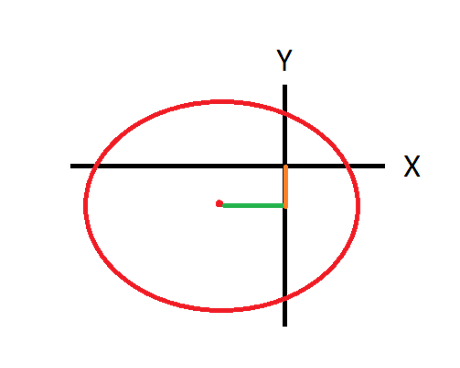
\includegraphics[scale=0.7,keepaspectratio=true]{pics/circle_offcenter.png}
    \caption{Kreis nicht im Ursprung}
    \label{fig:circle_offcenter}
\end{figure}
Um jeden Messpunkt zu erhalten, muss der Sensor einmal um alle Achsen gedreht werden.
Der entstehende Kreis ist ohne Kalibrierung nicht zentral im Koordinatensystem platziert.
Ziel ist es, den Kreis in den Koordinatenursprung zu verschieben.
\autoref{fig:circle_offcenter} zeigt nicht kalibrierten Zustand und \autoref{fig:circlecenter} den korrekt verschobenen Kreis.
\begin{figure}[htpb] % {H}
    \centering
    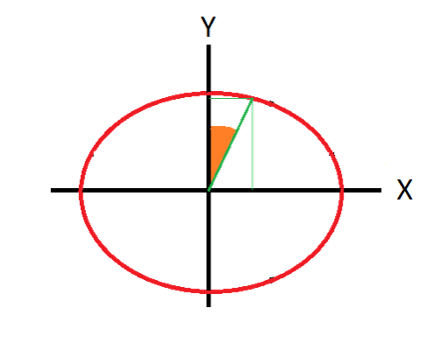
\includegraphics[scale=0.7,keepaspectratio=true]{pics/circle_center.png}
    \caption{Kreis im Ursprung}
    \label{fig:circlecenter}
\end{figure}

Für die Kalibrierung werden die Kompasswerte im Programmcode mehrmals pro Sekunde abgefragt und in Variablen gespeichert.
Dabei gibt es für jede Achse einen Minimal- und Maximalwert.
Nachdem der Kompass um alle drei Achsen gedreht wurde, sind die sechs Werte erfasst.
Anschließend muss daraus der jeweilige Korrekturfaktor für die einzelnen Achsen abgeleitet werden.
Ziel ist es, den Minimal- und Maximalwert für die Berechnung der Nordausrichtung im gleichen Abstand links und rechts des Koordinatenursprungs zu setzen, wie in \autoref{fig:circle_offcenter} gezeigt.
Dabei werden pro Achse die Maximalwerte und die Minimalwerte addiert und diese Summe halbiert.
Nun hat man die nötigen Korrekturfaktoren für die Kalibrierung und kann diese mit den x-, y- und z-Werte verrechnen.
Eine Eigenschaft des QMC5883L-Kompassmodul ist, dass dieses nicht ständig neu kalibriert werden muss.

\subsubsection{Servomotoren}
\chapterauthor{Felix Wagner}
Bei den Servomotoren handelt es sich um Analogservos der Firma Bluebird mit der Bezeichnung BMS-L530MG.
Diese benötigen eine Spannung von 4.5 V bis 6.5 V werden über ein PWM-Signal gesteuert.
Dieses Steuersignal hat eine Frequenz von 250 Hz und stellt den Servomotor bei einem Dutycycle von 1330 µs in seine mittlere Stellung.
Gegen den Uhrzeigersinn kann mit einem Dutycycle von 900 µs auf 60° gestellt werden.
Gleichfalls kann mit dem Dutycycle 2100 µs der Aktionsradius im Uhrzeigersinn gefahren werden.
Damit ergibt sich ein Gesamtaktionsbereich von 120°. \autocite{servomotor}

\paragraph{Ansteuerung}

\begin{figure}[htpb] % {H}
    \centering
    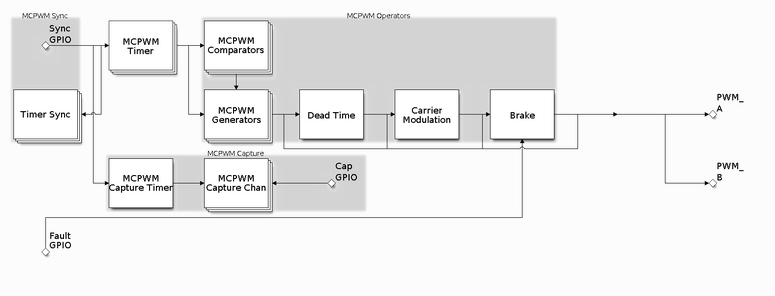
\includegraphics[scale=0.7,keepaspectratio=true]{pics/mcpwmOverview.png}
    \caption{MCPWM Überblick}
    \label{fig:mcpwmOverview}
\end{figure}

Die Generierung des PWM-Signals wird vom Neben-ESP übernommen.
Dafür wurde die MCPWM-Bibliothek verwendet.
\autocite{fig:mcpwmOverview} zeigt den Aufbau der Treiberbibliothek
Die folgenden Komponenten werden benötigt:

\begin{itemize}
    \item Timer: Zeitbasis des PWM-Signals
    \item Comparator: Vergleicht Zähler der Zeitbasis mit Schwellenwert und löst ein Vergleichsereignis aus
    \item Compare Event: Gibt das Verhalten vor, das bei einem positiven Vergleichen mit dem Dutycycle ausgeführt werden soll
    \item Generator: Generiert das PWM-Signal
    \item Operator: Modul, welches den Comparator und Generator zusammenführt, und somit die Signalerzeugung steuert
\end{itemize}

Der Timer wird mit einer Genauigkeit von 1 µs und einer Periode von 4000 eingestellt.
Dies entspricht 250 Hz.
Anschließend werden Comparator und Generator erstellt und mit dem Operator verknüpft.
Dann wird der Generator mit Verhaltensweisen konfiguriert, welche ausgeführt werden, wenn das Timerereignis und das Vergleichsereignis auftreten.
Tritt das Timerereignis auf, so wird das Signal am Portausgang auf \emph{HIGH} gesetzt.
Tritt nun das Vergleichsereignis auf, bei dem der Zeitzähler mit dem Wert des Dutycycles übereinstimmt, so wird der PWM-Port wieder auf \emph{LOW} gesetzt.
Der gewünschte Dutycycle wird durch die folgende Formel berechnet:

\[Dutycycle = angle_{required} \cdot \frac{PWM_{upper} - PWM_{lower}}{angle_{max}} + PWM_{lower} \]


\paragraph{Abdeckungsbereich}
Um die Solarpanele unabhängig der Sonnenposition ausrichten zu können, ist ein Gesamtaktionsbereich der Solarpanele von 360° Rotation nötig.
Jedoch besitzen die verbauten Servomotoren nur einen Aktionsradius von 120°. Da die Solarpanele so verbaut sind, dass sie sich in beide Richtungen gleich weit kippen lassen,
kann der Aktionsbereich verdoppelt werden.
Es verbleibt jeweils eine 60° breite Lücke auf beiden Seiten.\\
Umgesetzt wird dies wie Folgt:
Eine Funktion erhält die gewünschten Winkelpositionen für den Rotations- und den Kippservomotor und transformiert diese zunächst auf einen Wertebereich von 0° bis 360°.
Wird nun ein Winkel größer 180° für den Rotationsservo erkannt, so wird dieser Winkel um 180° verringert und zugleich vom Kippwinkel 180° abgezogen.
Damit kann fast die vollständige Abdeckung erreicht werden.

Anschließend wird der Berechnete Dutycycle vom maximalen höchsten Dutycycle abgezogen, um die Motoren mit steigendem Winkel gegen den Uhrzeigersinn drehen zu lassen.
Somit verhält sich der Ansteuerwinkel analog zu den Winkeln der Sonnenposition.

Um den Abdeckungsbereich der Servomotoren weiter zu erhöhen, wurde der minimale Dutycycle von 900 µs auf 820 µs verringert und der maximale Wert von 2100 µs auf 2150 µs erhöht.
Somit konnte der Abdeckungsbereich von 120° auf 160° erweitert werden.

\paragraph{Verbesserungen}
Die Servomotoren haben einige Probleme verursacht.
Die Anfangs gewählten Modelcraft ES-05 hatten durch ihre mangelhafte Dokumentation für großen Aufwand beim Suchen der korrekten Ansteuerung geführt.
Jedoch erwiesen sich diese Motoren für den Aufbau als zu schwach.
Somit musste auf die L530MG ausgewichen werden, welche jedoch nur einen Aktionsbereich von 120° gegenüber den 180° der ES-05 bieten. \\

Eine gute Alternative zu den Servomotoren wären Steppermotoren gewesen.
Diese hätten sich ebenfalls mit definierten Schritten mit ausreichender Genauigkeit positionieren lassen können.
Die günstigste Option hätte womöglich eine Kombination aus Linearmotor für die Rotation und Servomotor für die Kippfunktion geboten.
Hierbei würde das Kippen der Solarpanele analog zum aktuellen Aufbau funktionieren.
Die Rotation würde über den nicht positionierbaren Linearmotor müsste über einen, auf der Rotationsplattform platzierten, Kompasssensor überwacht werden.
Dabei muss zusätzlich auch auf mögliche Kabelverdrehungen geachtet werden, da beliebig weite Drehungen möglich sind.


\subsubsection{DCF-77}
\chapterauthor{Matthias Unterrainer}
DCF-77 ist ein weit verbreiteter Langwellenzeitcode in Mitteleuropa. Er wird von der von der Physikalisch-Technischen Bundesanstalt (PTB) aus Frankfurt, Deutschland, betrieben. Der DCF-77 sendet ein Zeit- und Datensignal auf einer Frequenz von 77,5 Kilohertz, wobei jede Sekunde ein Bit übertragen wird, also insgesamt 60 Bit pro Minute, was einem Datensatz entspricht. \cite{dcf77_logs}
\begin{figure}[htpb] % {H}
    \centering
    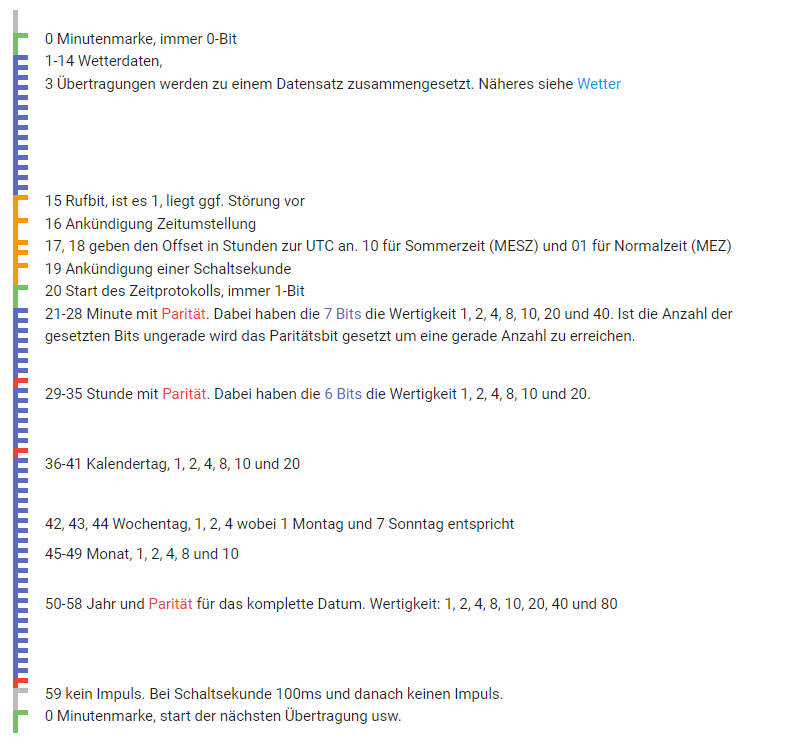
\includegraphics[width=15cm,keepaspectratio=true]{pics/dcf77_minute.png}
    \caption{Aufbau einer Minute. \cite{dcf77_logs}}
    \label{fig:dcf77_minute}
\end{figure}
Wie in \autoref{fig:dcf77_minute} zu erkennen besteht ein Datensatz grob aus Wetterdaten und der aktuellen Zeit, die sich aus Datum und Uhrzeit zusammen setzt, und noch einigen weiteren Informationen über beispielsweise Sommer-/Winterzeit.
Täglich werden dabei 480 Wetterdatensätze für 90 Regionen gesendet, wobei 60 Regionen eine Vier-Tage-Vorhersage und 30 Regionen eine Zwei-Tagen-Vorhersage erhalten. Die Übertragung der Wetterdaten beginnt täglich um 22 Uhr UTC mit Region 0. Für die ersten 60 Regionen werden für die ersten drei Tage sowohl die Höchst- als auch die Tiefstwert übertragen, während am 4. Tag nur noch der Höchstwert gesendet wird. Die freien Kapazitäten, die durch das Weglassen des Tiefstwerts am 4. Tag entstehen, werden genutzt, um für die restlichen 30 Regionen die Höchstwerte für die nächsten zwei Tage zu übermitteln. Ein ''Wetterbericht'' setzt sich dabei aus jeweils drei Einzelübertragungen zusammen. \cite{dcf77_wetter}
\begin{figure}[htpb] % {H}
    \centering
    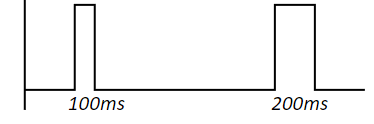
\includegraphics[width=0.5\textwidth,keepaspectratio=true]{pics/dcf77_signal.png}
    \caption{Vom DCF77-Reciever auslesbares Signal. \cite{dcf77_logs}}
    \label{fig:dcf77_signal}
\end{figure}
In Abb. \ref{fig:dcf77_signal} ist das vom DCF-77 Reciever Modul ausgegebene Signal zu sehen. Wobei deutlich zu erkennen ist, dass zum Beginn einer Sekunde der Ausgang entweder für 100ms (bei einem 0-Bit) oder 200ms (bei einem 1-Bit) auf \textit{HIGH} gezogen wird und dann für die restliche Sekunde auf \textit{LOW} bleibt. Um dieses Signal ordnungsgemäß auslesen zu können, müsste es gemäß dem Abtasttheorem mit mindestens 20 Hz abgetastet werden, da das kürzeste Signal 100 ms lang ist, also mit einer Frequenz von 10 Hz läuft. Dies würde jedoch bedeuten, dass der DCF-77-Lesetask mindestens alle 50 ms oder sogar noch häufiger gestartet werden müsste, um sicherzustellen, dass das Signal korrekt erkannt wird. Um allerdings genutzt werden zu können, müsste dieser Task auf dem Haupt-ESP laufen, da ansonsten aufgrund der Tatsache, dass die Kommunikation vom Haupt-ESP zum Neben-ESP unidirektional ist, die vom DCF-77 gelieferten Daten größteils ungenutzt bleiben würden. Auf dem Haupt-ESP werden jedoch bereits einige andere wichtige Tasks ausgeführt und das ständige starten des DCF-77 Tasks hat zu erheblichen Problemen beim Scheduling geführt, da der DCF-77 Task für mindestens eine ganze Minute ein sauberes Signal erkennen muss, um eine genaue Messung zu ermöglichen. Dies hat verhindert, dass der DCF-77 Task kontinuierlich laufen kann. 
Es wurde die Idee diskutiert, den Task nur zu bestimmten Uhrzeiten am Tag laufen zu lassen, um nur den ''Wetterbericht'' für die entsprechende Region vom DCF-77 zu erhalten, da die Uhrzeit sowieso viel genauer vom GPS empfangen wird, in Sekunden statt nur in Minuten wie beim DCF-77. Da allerings wie bereits erwähnt, ein einzelner ''Wetterbericht'' aus drei vollständigen Übertragungen besteht, die alle empfangen werden müssen, was mindestens drei Minuten in anspruch nehmen würde, und dabei den Haupt-ESP nahezu vollständig blockieren würden, wurde entschieden, den DCF-77 nicht einzubauen.

\chapterauthor{Matthias Unterrainer}

\subsubsection{LCD Display}
\chapterauthor{Matthias Unterrainer}
Das verwendete LCD Display hat eine Anzeige von 20 Zeichen über 4 Zeilen und kann sowohl im 8Bit Modus, als auch im 4Bit Modus betrieben werden.
Es wird mit einer Spannung von 5V versorgt und schaltet sich automatisch nach 1 Minute aus, wenn keine Eingaben durch die Knöpfe erfolgen.
Um Pins zu sparen, wird der 4 Bit Modus genutzt. Dabei werden beim Senden eines Zeichens zunächst die oberen 4 Bit und anschließend die unteren 4 Bit an das Display gesendet. Da jeder Sendevorgang etwa 200 $\mu$s dauert, verdoppelt sich dadurch die Übertragungszeiten. Da der Task über FreeRTOS nicht für derart kurze Zeitspannen inaktiv gesetzt werden kann, mussten diese durch eine Busy-Waiting-Implementierung umgesetzt werden.\\\\
Zusätzlich bietet das LCD Display die Möglichkeit, den Hintergrundkontrast einzustellen. Hierzu wird eine Spannung zwischen 0V und $V_{\text{DD}}$ an den entsprechenden Pin angelegt. Diese Einstellung kann mithilfe des am Steuerbrett, zwischen den Knöpfen, angebrachten Potenziometer vorgenommen werden.\\
Des Weiteren wird die Hintergrundbeleuchtung des Displays ebenfalls vom Neben-ESP gesteuert. Die Versorgungsspannung der Anode des LCD-Display-Moduls ist mit dem GPIO-Pin 13 verbunden, wodurch es zwischen 0V (ausgeschalten) und 3.3V (eingeschalten) umgeschaltet werden kann, und zusammen mit dem Display ein- oder ausgeschalten.

\subsubsection{Knöpfe}
\chapterauthor{Matthias Unterrainer}
Die Knöpfe für das LCD Menu sind über \textit{HIGH} mit dem Neben-ESP verbunden. Für den linken Knopf musste zudem ein externer Pull-Up Widerstand eingebaut werden, da er über den GPIO-Pin 36 läuft, der keine internen Pull-Up/Pull-Down Widerstände hat. Die Knöpfe werden alle 200 $\mu$s abgefragt und können folgende 3 verschiedene Zustände einnehmen:\\
\begin{tabular}{l|c|c}
%\backslashbox{Aktion}{Gedrückte Buttons}    & Button0       & Button1   \\
\hline
NEXT                                        & \checkmark    &           \\
PREV(ious)                                  &               & \checkmark\\
CONF(irm)                                   & \checkmark    & \checkmark\\
\end{tabular}\\
\textit{NEXT} führ dabei zum Vorspringen zum nächste Element im Menü, während \textit{PREV} zum Zurückspringen dient. Ursprünglich wurde \textit{CONF} verwendet um den aktuell angezeigten Wert zu ändern. Nach dem Umzug auf den Neben-ESP war dies jedoch nicht mehr möglich. Nun reinitialisiert \textit{CONF} das LCD Display und lädt die Diplay Konfiguration, die über die Web-Gui eingestellt wird, neu.

\subsection{Algorithmen}
\chapterauthor{Matthias Unterrainer}

\subsubsection{Ausrichtung der Panels}
\chapterauthor{Felix Wagner}
Die Ausrichtung der Solarpanele erfolgt über die vom Haupt-ESP berechneten Azimut und Elevation Werte.
Diese repräsentieren die Position der Sonne am Himmel. 
Wenn davon ausgegangen wird, dass der SunStorage Aufbau stets auf einer ebenen Fläche liegt, dann können die Azimut- und Elevationwerte direkt auf die Postionen der Rotations- und Kippservos übertragen werden. 
Somit würde sich eine direkte Ausrichtung zur Sonne ergeben und die Effektivität der Solarpanele wäre maximiert.
Dieser Fall ist jedoch im praktischen Betrieb nicht immer gegeben.

\subsubsection{Schieflage des Systems}
Steht der Aufbau schief, so ist die Trennung der Aufgabengebiete des Rotieren und Kippens der Solarpanele nicht mehr gegeben.
Somit können die Azimut und Elevation nicht mehr direkt für die Stellung der Servomotoren verwendet werden.
Kippt man etwa den kompletten Aufbau auf eine Seite, so sind die Aufgaben der Motoren komplett umgekehrt.
Für alle Orientierungen dazwischen übernehmen die Motoren Rotation und Kippen gemeinsam.

\paragraph{Beschleunigungswerte}
Um die Lage des SunStorage Systems zu ermitteln, muss die Erdbeschleunigung anhand von drei Achsen gemessen werden. 
Dies erfolgt über die Daten des Beschleunigungssensors.

\paragraph{Interpretation der Beschleunigungswerte}
Betrachtet man die Beschleunigungswerte der drei Achsen als Vektor im 3-dimensionalen Raum, 
so spannt dieser Vektor eine Ebene auf. 
Dieser Vektor muss nun an der z-Achse im Koordinatensystem gespiegelt werden. 
Damit lässt sich die physikalische Lage von SunStorage im Koordinatensystem abbilden.
Dieser Vektor wird im weiteren Verlauf $ V_{SunStorage} $ genannt.

\paragraph{Darstellen der Sonne im Koordinatensystem}
Nachdem nun SunStorage im Koordinatensystem abgebildet ist, muss die gewünschte Sonnenposition mittels eines Vektors hinzugefügt werden.
Wie bereits bekannt wird die Sonnenposition über die Werte Azimut und Elevation angegeben. 
Dabei handelt es sich um Winkel. 
Diese können mithilfe der trigonometrischen Funktionen in einem 3-dimensionalen Vektor übersetzt werden.
Hierfür wird die Berechnung in vier verschiedene Fälle aufgeteilt, welche die vier Quadranten eines 2-dimensionalen Koordinatensystems darstellen. 
\begin{itemize}
    \item I Quadrant: $x = 1 y = \tan(Azimuth)$
    \item II Quadrant: $x = -1 y = -\tan(Azimuth)$
    \item III Quadrant: $x = -1 y = -\tan(Azimuth)$
    \item IV Quadrant: $x = -\tan(Azimuth) y = -1$
\end{itemize}
Anschließend wird der Vektor aus dem Punkt (x,y) und dem Ursprung normalisiert, um mit dem später berechneten z-Wert die Sonnenposition darzustellen.\\
Die z-Koordinate wird anschließend über den Tangens des Elevationwertes bestimmt. 

$$ z = \tan(Elevation) $$

Nun stellen x, y und z den Sonnenvektor $ V_{Sonne} $ dar.\\
Ist der Elevationswinkel 90°, so wird $ V_{Sonne} $ auf (0,0,1) gesetzt, da in diesem Fall der Azimutwert vernachlässigbar ist.
Nun kann die Sonnenposition im Koordinatensystem dargestellt werden.

\paragraph{Solarpanele darstellen}
Um die Orientierung der Solarpanele im Koordinatensystem darzustellen, wird eine Ebene konstruiert, welche die Panele senkrecht in ihrer Mitte trennt.
Diese wird über die Berechnung des Orthogonalvektors der z-Achse und $ V_{SunStorage} $ bestimmt:
\[
\begin{pmatrix}
    0\\
    0\\
    1\\
\end{pmatrix}
\times
V_{SunStorage}
=
V_{ortho}
\]
Aus dem Vektor $ V_{ortho} $ lässt sich die Koordinatenform als Ebene erstellen.
\[V_{ortho}x \cdot x + V_{ortho}y \cdot y + V_{ortho}z \cdot z = 0\] 
Nun kann diese Ebene um die Achse von $ V_{SunStorage} $ rotiert werden.
Dies wird über die allgemeine Drehmatrix umgesetzt.
\[
R_n(\alpha)
=
\begin{pmatrix}
    n^2_1(1-\cos\alpha)+\cos\alpha & n_1n_2(1-\cos \alpha)-n_3\sin\alpha & n_1n_3(1-\cos\alpha)+n_2\sin\alpha\\
    n_2n_1(1-\cos\alpha)+n_3\sin\alpha & n^2_2(1-\cos\alpha)+\cos\alpha & n_2n_3(1-\cos\alpha)-n_1\sin\alpha\\
    n_3n_1(1-\cos\alpha)-n_2\sin\alpha & n_3n_2(1-\cos\alpha)+n_1\sin\alpha & n^2_3(1-\cos\alpha)+\cos\alpha\\
\end{pmatrix}    
\]
An Stelle von $ n = (n_1, n_2, n_3)^T $ wird $ V_{SunStorage}^T $ eingesetzt.
Dies entspricht der Bewegung des Rotationsservomotors.
Anschließend kann die Rotation der Ebene gesucht werden, für die $ V_{Sonne} $ eingesetzt
in  die Koordinatenform der Ebene des Normalenvektors $ V_{ortho} $ den geringsten Wert hat. %TODO der satz doof
Damit ist die Bestimmung der Stellung des Rotationsmotors beendet, da dies bedeutet, 
dass $ V_{Sonne} $ in der Ebene von  $ V_{ortho} $ liegt.
Anschließend erfolgt die Berechnung der Stellung des Kippmotors.
Dafür wird ein weiterer Orthogonalvektor $ V_{opt} $ erzeugt. 
Dieser liegt zwischen der z-Achse und $ V_{ortho} $. 
Die Stellung des Kippmotors kann somit durch die Berechnung des Winkels zwischen $ V_{opt} $ und $ V_{Sonne} $ bestimmt werden:
\[\alpha = \arccos(\frac{V_{opt} \cdot V_{Sonne}}{\left| V_{opt} \right| \cdot \left| V_{Sonne} \right|})\]

\subsubsection{Schieflage des Kompass}
Der Kompass liefert in Abhängigkeit seiner Ausrichtung unterschiedliche Werte.
In diesem Kapitel wird die notwendige Korrektur beschrieben.
\paragraph{Nordausrichtung}
\chapterauthor{Felix Wagner}
Die Bestimmung der Orientierung zu Norden erfolgt über die Winkelberechnung zwischen der 
y-Achse und der Geraden des Koordinatenursprungs und des aktuellen (x, y)-Messpunkts. 
Dieser Winkel wird mittels der Tangensfunktion ermittelt. Siehe Abbildung \autoref{fig:circlecenter}.
Die C Standardbibiliothek $math.h$ liefert hierfür die Funktion $atan2f$, 
welche den Winkel als float Datentyp zurückgibt 
und die vier verschiedenen Quadranten des Koordinatensystems berücksichtigt.

\paragraph{Schieflagenkorrektur}
\chapterauthor{Felix Wagner}
Es ist nicht immer gegeben, dass der Kompass perfekt gerade liegt. 
Deshalb müssen die Sensorwerte unter Berücksichtigung des vom Beschleunigungssensor 
gestelltem Orientierungsvektor angepasst werden. 
Dies erfolgt über die sogenannte Vektorprojektion. 
Dabei wird über folgende Formel \[\vec{a_{projected}} = \frac{\vec{a} \circ \vec{b}}{\vec{b} \circ \vec{b}} \cdot \vec{b} \]
der Vektor aus den Kompasswerten auf die Orientierung des Vektors der Beschleunigungswerte projeziert. 
Anschließend werden die x- und y-Werte des projezierten Vektors von denen des Kompassvektors subtrahiert. 
Somit sind die Kompasswerte bereit für die oben besprochene Weiterverarbeitung.

\subsubsection{Verbesserter Algorithmus}
Der implementierte Algorithmus nutzt für seine Berechnung viele Multiplikationen und trigonometrische Funktionen.
Dies erzeugt einen großen Rechenaufwand und ist im Dauerbetrieb nicht optimal.
Dies wirkt sich aufgrund der großen zeitlichen Abstände der Funktionsaufrufe kaum negativ auf die Funktionsweise von SunStorage aus.
Im Folgenden wird eine effizientere Formel erklärt.\\
Die Berechnung von $ V_{SunStorage} $  und $ V_{Sonne} $ erfolgt analog zum ursprünglichen Algorithmus.
Anstatt einer Ebene für die Solarpanele eine Ebene über den Vektor $ V_{SunStorage} $ in Koordinatenform erzeugt.
\[V_{SunStorage}x \cdot x + V_{SunStorage}y \cdot y + V_{SunStorage}z \cdot z = 0\] 
Anschließend wird die Spitze von $ V_{Sonne} $ als Ausgangspunkt für eine Gerade $ G_{Sonne} $ mit dem Richtungsvektor $ V_{SunStorage} $ generiert.
Der Schnittpunkt von $ G_{Sonne} $ mit der Ebene von SunStorage stellt mit dem Ursprung des Koordinatensystems den Vektor $ V_{opt} $ dar.
Aus $ V_{opt} $ kann wiederum die Stellung für Rotation und Kippen der Motoren analog zum vorherigen Ansatz berechnet werden.

\subsubsection{Bestimmung der Abweichung zum Norden}
\chapterauthor{Felix Wagner}
Die Bestimmung der Orientierung zu Norden erfolgt über die Winkelberechnung zwischen der 
y-Achse, der Geraden des Koordinatenursprungs und des aktuellen (x, y)-Messpunkts. 
Dieser Winkel wird mittels der Tangensfunktion ermittelt. (siehe \autoref{fig:circlecenter})
Die C Standardbibliothek $math.h$ liefert hierfür die Funktion $atan2f$, 
welche den Winkel als float Datentyp zurückgibt und dabei die vier verschiedenen Quadranten des Koordinatensystems berücksichtigt.

\paragraph{Schieflagenkorrektur}
Es ist nicht immer gegeben, dass der Kompass perfekt gerade liegt. 
Deshalb müssen die Sensorwerte unter Berücksichtigung des Orientierungsvektors, die der Beschleunigungssensor liefert, angepasst werden. 
Dies erfolgt über eine Vektorprojektion.
Mithilfe der folgenden Formel wird der Vektor aus den Kompasswerten auf die Orientierung des Vektors der Beschleunigungswerte projiziert.
\[\vec{a_{projected}} = \frac{\vec{a} \circ \vec{b}}{\vec{b} \circ \vec{b}} \cdot \vec{b} \]
 
Anschließend werden die x- und y-Werte des projizierten Vektors von den Werten des Kompassvektors subtrahiert. 
Somit sind die Kompasswerte bereit für die in Weiterverarbeitung. \autocite{compasstilt}

\subsubsection{Nachtabschaltung}
\chapterauthor{Matthias Unterrainer}
Um möglichst viel Energie zu sparen, wurde eine Nachtabschaltung implementiert. Diese führt dazu, das in er Zeit von einer Stunde nach dem Sonnenuntergang bis eine Stunde vor dem Sonnenaufgang, die Solarpanele in eine vorher über die Web-GUI festgelegte Position eingestellt werden, der Task zur ausrichtung der Panele blockiert und ein globales Event \textit{Nachtabschaltung} gesetzt wird, wodurch auch andere Task von der Nachtabschaltung informiert werden.

% Die Berechnung für die Sonnenauf/untergangszeiten basieren auf diesem, ursprünglich vom Nautical Almanac Office veröffentlichen Algorithmus, \cite{nachabschaltung_algo}. Dieser benötigt lediglich den aktuellen Längen-/Breitengrad und das aktuelle Datum, Monat und Tag. 
% Dazu wird zuerst vom Datum, also Monat und Tag, der aktuelle Tag des Jahres berechnet, d.h. der 1.1 ist Tag 1 und der 15.4 ist Tag 74. Dannach wird der Längengrad in Stunden umgerechnet und 

\subsubsection{Akkuladegerät}\label{Akkuladegerät}
\chapterauthor{Lukas Eigenstetter}
Der Algorithmus des Akkuladegerätes kann durch die State Machine in \autoref{stmAkkulader} beschrieben werden.
\begin{figure}[htpb] % {H}
    \centering
    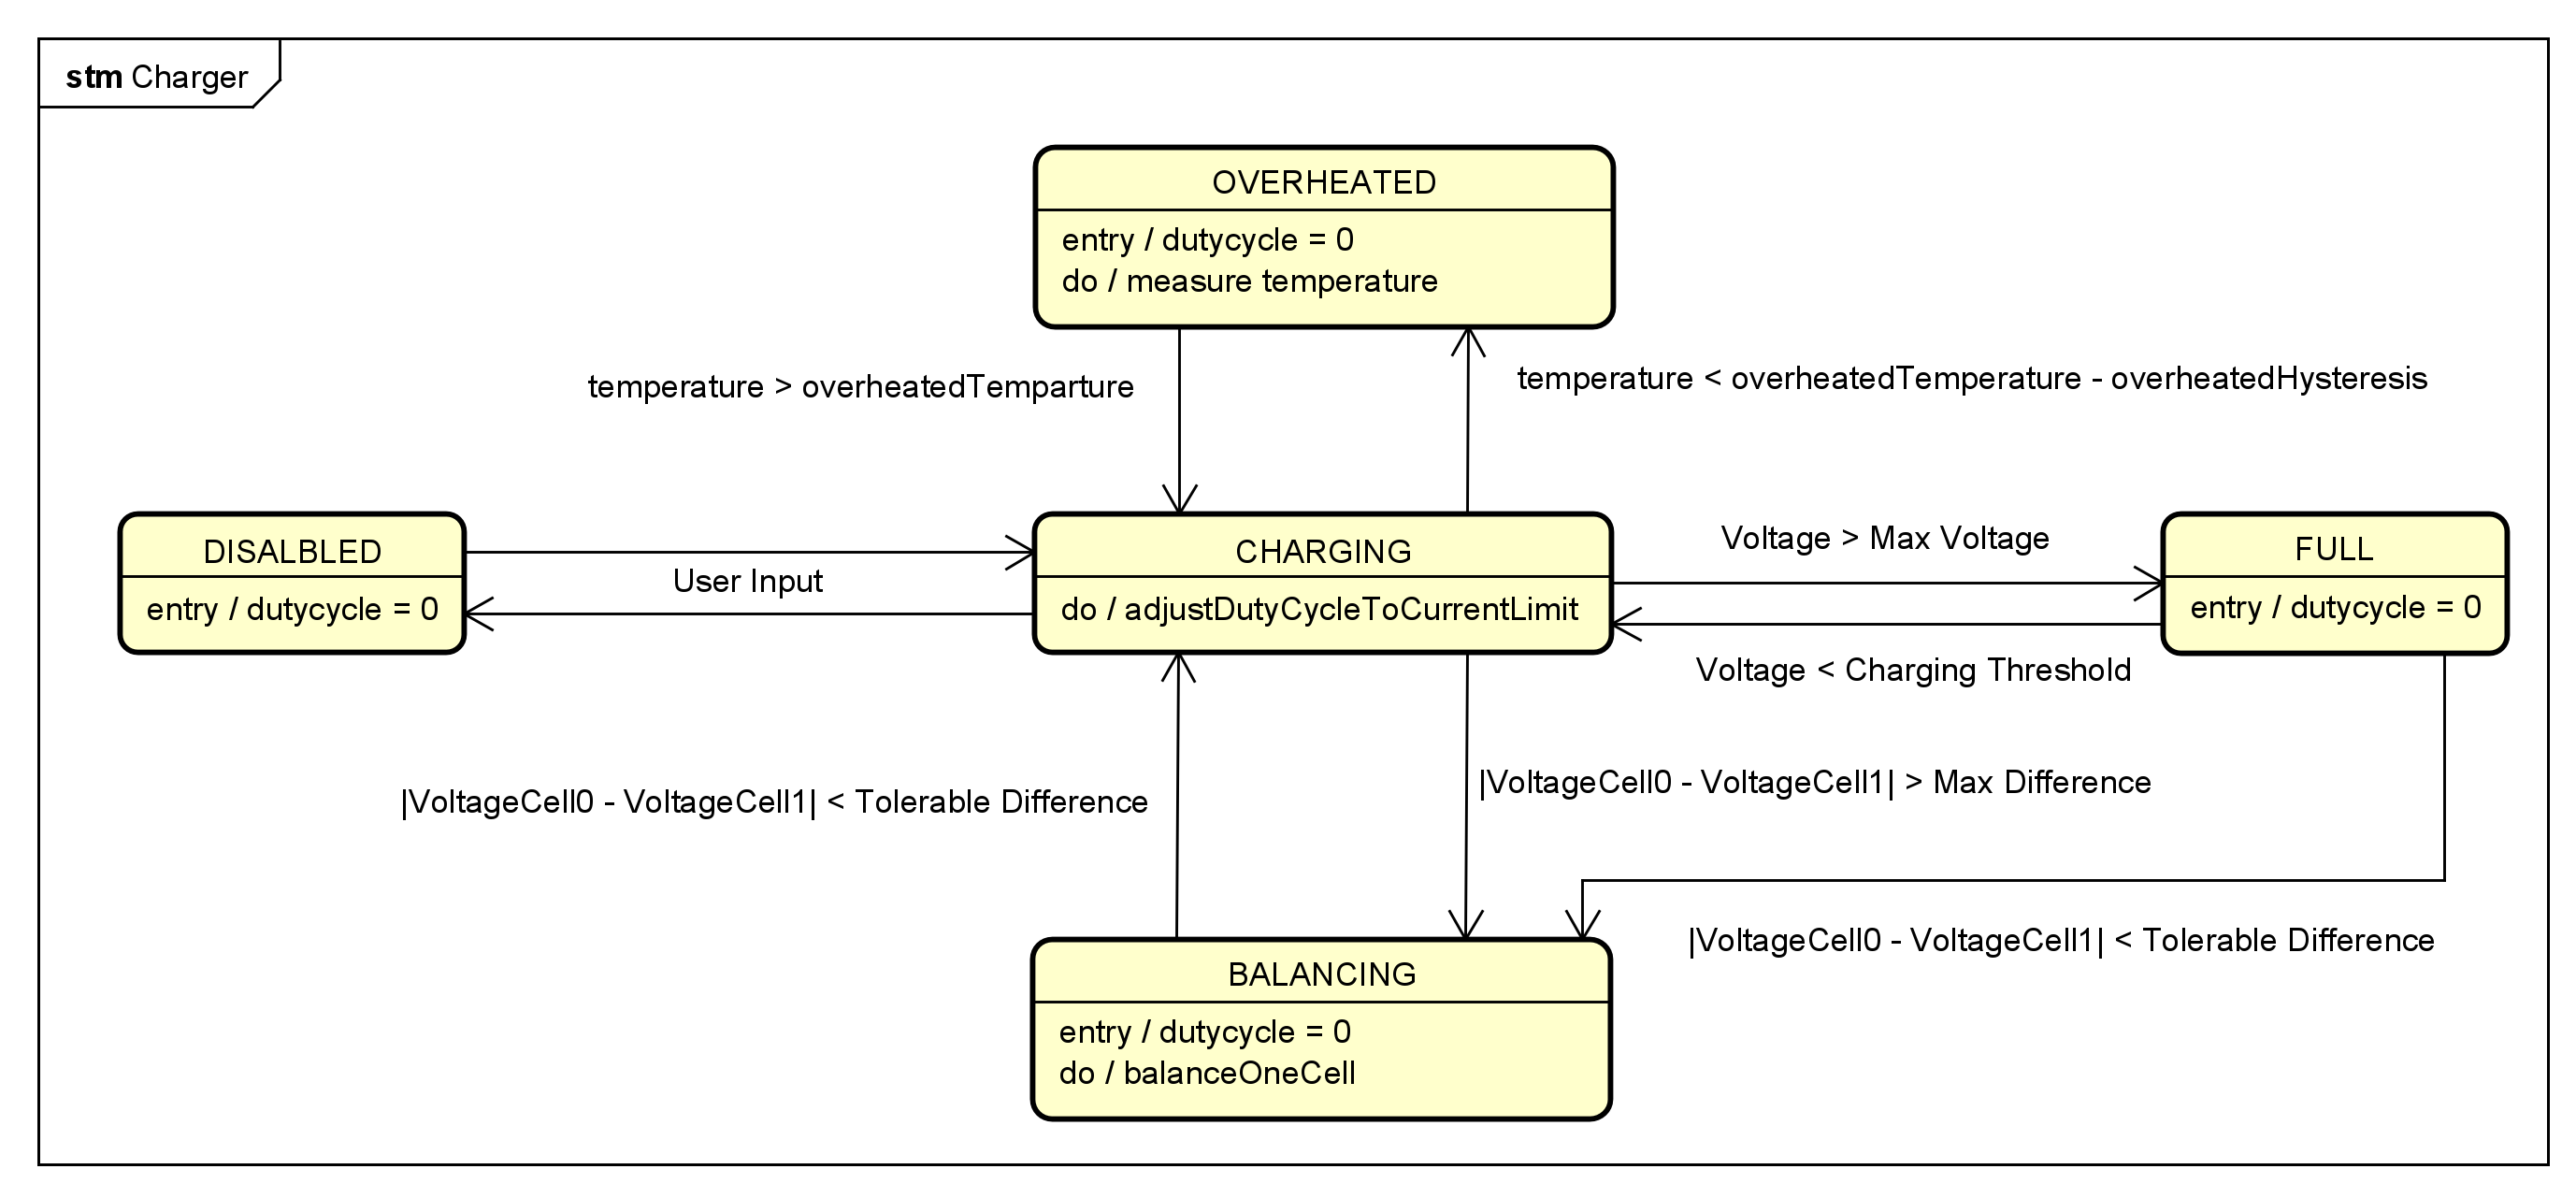
\includegraphics[width=\textwidth,keepaspectratio=true]{pics/chargerStm.png}
    \caption{State Chart zum Ladealgorithmus}
    \label{stmAkkulader}
\end{figure}
Der zentrale Zustand ist der Zustand \emph{CHARGING}.
In diesem wird das PWM, dessen Schaltung in \autoref{akkuCircuit} beschrieben ist, angepasst.
In allen anderen Zuständen ist der Duty Cycle 0.
Das Ladegerät kann durch den Nutzer im Frontend gestartet oder gestoppt werden.
Im Zustand \emph{CHARGING} wird zusätzlich der Temperatursensor geprüft.
Falls die Temperatur über einem festgelegten Wert liegt, so wird der Zustand \emph{OVERHEATED} angenommen.
Dies dient zum Schutz der Batterie vor zu hohen Temperaturen.  \autocite[S. 53]{chargerBuch}
Falls die Batterie eine gewisse Spannung überschreitet, nimmt das Ladegerät den Zustand \emph{FULL} ein.
So kann ein Laden bis zu einer gewissen Grenze ermöglicht werden.
Im Zustand \emph{BALANCING} wird die vollere der beiden Zellen über einen Widerstand entladen.
Eine detaillierte Beschreibung der Notwendigkeit dieses Verfahrens ist im \autoref{akkuCircuit} beschrieben.
Um häufiges Wechseln zwischen den Zuständen zu vermeiden, sind jeweils Hysteresen definiert.\\
Eine Abschaltung des Systems bei zu niedrigem Ladestand wurde nicht eingebaut, da dies eine relativ schwierige Aufgabe ist.
Um zu messen, ob eine Spannung unterschritten wird, muss das System eingeschaltet sein.
Sinnvoll wäre daher eine analoge Lösung.
Diese könnte durch einen Transistor realisiert werden, der anhand eines Spannungsteilers gesteuert wird.
Das Problem bei dieser Lösung ist, dass die Schaltung nicht im Betrieb konfiguriert werden könnte.
Bei Betrieb mit NiMH Batterien würde dies dazu führen, dass der Ausschaltvorgang an einer falschen Stelle eintritt.\\

Der Ladestrom wird über ein 13 Bit PWM Signal geregelt.
Das Signal wird jeweils um die Differenz des zuletzt gemessenen Stromes in mA und dem derzeitigen PWM Wert angepasst:
$$ PWM_{neu} = PWM_{alt} + (I_{Ziel} - I_{Charger}) \cdot PWM\_REGULATION\_FACTOR $$
Der Wert Reglerkonstante $ PWM\_REGULATION\_FACTOR $ ist 1.\\
Der Zielwert des Ladestroms kann durch den Nutzer mithilfe des Wertes \emph{currentTarget} vorgegeben werden.
Dieser wird bis zum Spannungswert \emph{trickleThreshold} verwendet.
Ab dem Spannungswert \emph{trickleThreshold} wird der Ladestrom $ I_{Ziel} $ linear verringert, bis er bei der \emph{maximumVoltage} auf 0 reduziert wurde.
Abbildung \autoref{ladekurve} zeigt den daraus resultierenden Verlauf für die Standardwerte.
\begin{figure}[htpb] % {H}
    \begin{center}
        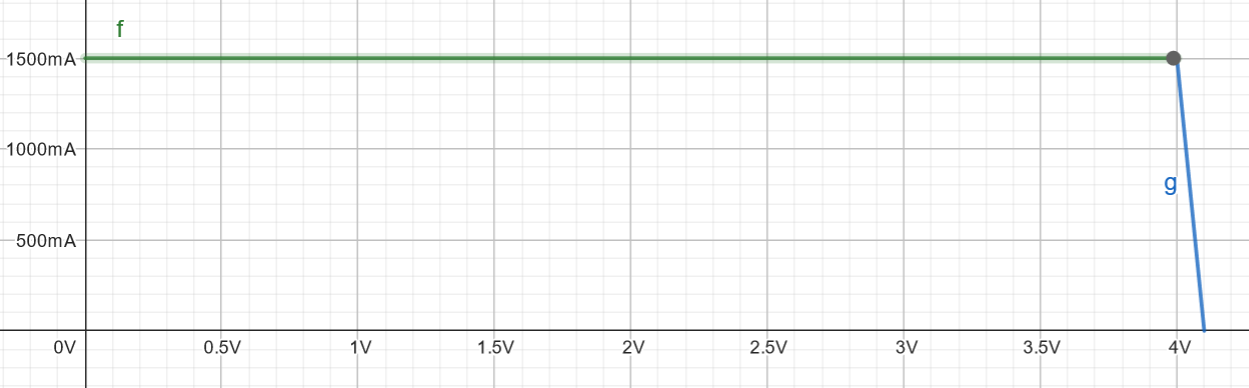
\includegraphics[width=13cm,keepaspectratio=true]{pics/ladekurve.png}
        \caption{Verlauf maximalen Ladestroms in Abhängigkeit der Zellenspannung}\label{ladekurve}
    \end{center}
    Die Darstellung zeigt den Verlauf für die Defaultwerte.
    Die Spannung ist immer pro Zelle zu betrachten.
\end{figure}

Die Gerade im Trickle-Bereich wird durch die folgende Gleichung beschrieben:
$$ I_{target} = I_{currentTarget} + I_{currentTarget} \cdot \frac{U_{trickleOffset}} {U_{trickleThreshold} - U_{maximumVoltage}} $$
Die Werte  $ U_{maximumVoltage} $, $ I_{currentTarget} $ und $ U_{trickleThreshold} $ können durch den Nutzer vorgegeben werden.
$ U_{trickleOffset} $ gibt an, an welcher Stelle des Trickle-Bereichs die Spannung gerade liegt.
Sie wird durch die folgende Gleichung bestimmt:
$$ U_{trickleOffset} = (U_{Battery} - U_{trickleThreshold} \cdot CELL\_COUNT) / CELL\_COUNT $$
Die Anzahl der Akkuzellen, $ CELL\_COUNT $, ist 2.
Professionelle Ladegeräte verwenden meist nicht-lineare Zielströme im Trickle-Bereich. \autocite[S. 50f]{chargerBuch}

\subsubsection{Ladezustandsabschätzung}\label{Ladezustandsabschätzung}
\chapterauthor{Lukas Eigenstetter}
Akkus haben die Eigenschaft, dass sie mit abnehmendem Ladezustand an Spannung verlieren.
Diesen Effekt kann man zur Abschätzung des Ladezustands (State of Charge Estimation) nutzen.
Ein einfaches Verfahren der Ladezustandsabschätzung kann die zuletzt gemessene Spannung der Batterie verwenden.
Da die Spannung der Zellen unter Last um bis zu 600 mV abnimmt, wird eine zusätzliche Metrik benötigt.\\
Diese wird durch die Messungen des Coulomb-Counters umgesetzt.
Durch ein- und abfließenden Strom kann auf die Veränderung des Ladezustands geschlussfolgert werden.
Die Strommessungen bieten jedoch keine Einsicht in den absoluten Ladezustand.
Daher wird ein hybrides Verfahren der Ladezustandsabschätzung umgesetzt, das beide Metriken verwendet:\\
Alle zehn Minuten wird der spannungsbasierte Kalibrierungstask aufgerufen.
In diesem werden High-Power-Circuit und Ladegerät ausgeschaltet, um einen möglichst geringen Strom im System zu haben.
Dann wird eine Millisekunde gewartet und die ADC werden ausgelesen.
Anhand eines separat bestimmten, nicht gemittelten Wertes der Batteriespannung wird durch einen Lookup in einer Wertetabelle der Ladezustand in Prozent bestimmt.
\autoref{socTable} zeigt die hierfür verwendete Tabelle.\\
\begin{figure}[htpb] % {H}
    \centering
    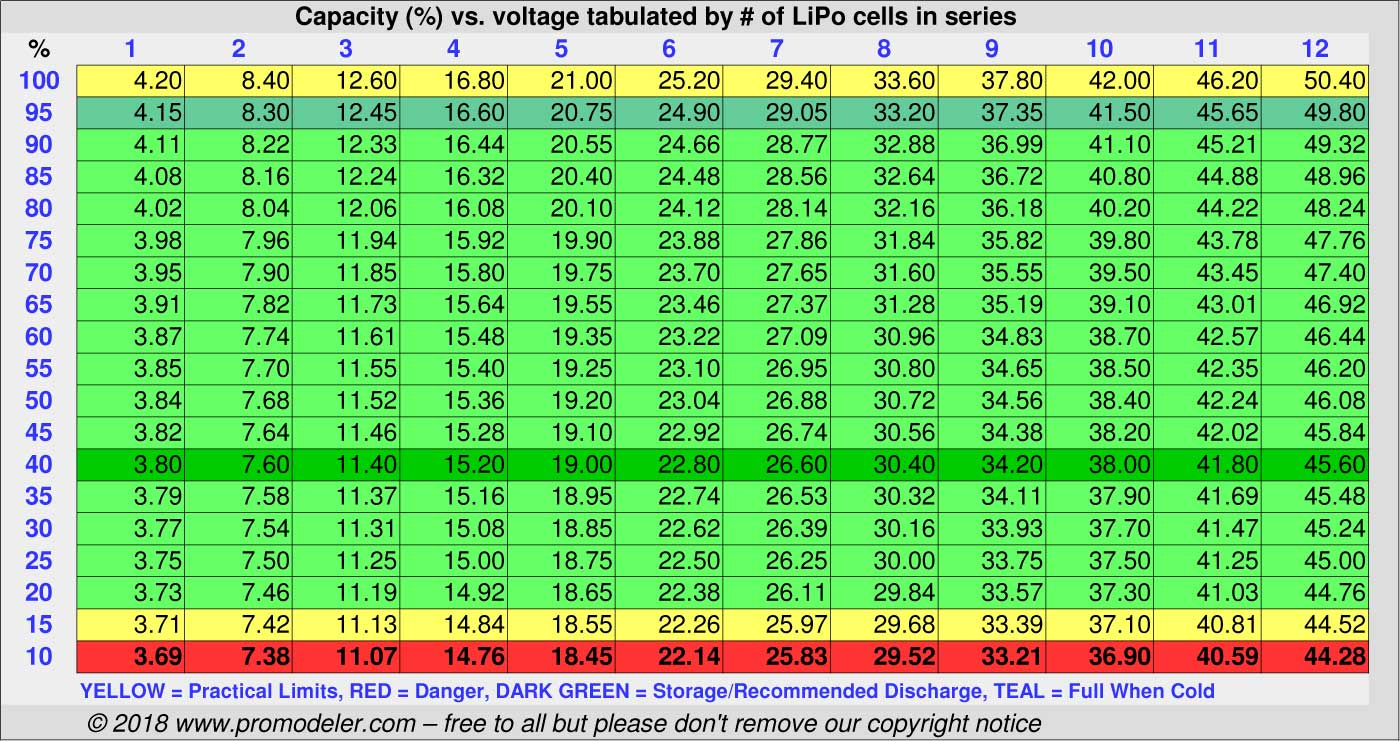
\includegraphics[width=13cm,keepaspectratio=true]{pics/socTable.jpg}
    \caption{Verwendete Tabelle für die Ladezustandsabschätzung \cite{socTable}}
    \label{socTable}
\end{figure}
Zu dieser wurde eine Umkehrfunktion bestimmt, um eine Abbildung von Spannung auf Ladezustandswerte zu erlauben.
Die Tabelle hat 100 Werte und erstreckt sich über den Spannungsbereich von 8.4 V bis 7.4 V.
Die Auflösung ist demnach teilweise höher als in der Tabelle.
In diesen Fällen wurde linear interpoliert.
Die Werte sind liegen im Programm als konstantes Array vor.
Durch die folgende Formel wird der Ladezustand aus der Spannung bestimmt mithilfe eines einzigen Zugriffs bestimmt:
$$ SoC = F_{SoC}((U_{Battery} - 7400) / 10) $$
$F_{SoC}$ ist hierbei die Wertetabelle und $U_{Battery}$ die Batteriespannung in Millivolt.
Im C-Code muss zusätzlich darauf geachtet werden, dass die Spannung im Bereich von 7.4 bis 8.4 V liegt.
Der Task, der für das Auslesen der ADC verantwortlich ist, verändert den Wert des Ladezustands anhand des produzierten und verbrauchten Stroms gemäß der folgenden Formel:\\
$$ SoC = SoC + \frac{Q_{CC} * 10}{K_{Bat}} $$ %TODO prüfen!!
$ Q_{CC} $ ist die gemessene Ladung in Coulomb und $ K_{Bat} $ ist die Kapazität des Akkus in Milliamperestunden.

In der Praxis ist der Stromverbrauch im Ruhezustand bereits hoch genug, um die Spannung der verwendeten Akkus signifikant zu verringern.
Die Kalibrierung liefert deutlich zu niedrige Werte.
Durch die Verwendung eines sparsameren Controllers für das Ladegerät und der Abschaltung aller Module könnte dieses Problem gelöst werden.\\
Da jedoch noch Bugs in Coulomb-Counter-Anpassung existieren, ist der gemessene Ladezustand immer 0. \autocite[S. 139 - 158]{chargerBuch}
\newpage
\section{Verbesserungsmöglichkeiten}
\chapterauthor{Lukas Eigenstetter}
Dieses Kapitel befasst sich mit den Verbesserungsmöglichkeiten im Projekt.
Die bei der Abnahme noch bestehenden Probleme der Teilkomponenten wurden bereits in den jeweiligen Unterkapiteln in \autoref{Dokumentation} beschreiben.
Außerdem werden einige Alternativen aufgezeigt, die zu einem besseren Ergebnis geführt hätten.

\subsection{Planung und Ablauf}
\chapterauthor{Lukas Eigenstetter}
Ein großes Problem in diesem Projekt war die Zeitplanung.
Die Phase der Integration wurde unterschätzt und entsprechend zu spät begonnen.
Bei der Zusammensetzung der Komponenten kamen viele Bugs zum Vorschein und neue Probleme traten auf.
Diese hätten meist durch Unit Tests, Schnittstellentests und frühere Komponenten erkannt werden können.
Außerdem wurde vergessen, die PINs für das SD-Card Modul zu vermerken, wodurch der Neben-ESP erst notwendig wurde.
Diese Fehler und Versäumnisse spiegeln sich in der hohen Stundenzahl ab Woche 13 wider.

% Lukas & Matthias
% kabeldämpfung, smt circuit designen usw...

\subsection{Mechanischer Aufbau}
\chapterauthor{Philipp Thaler, Felix Wagner und Lukas Eigenstetter}
Durch das Verwenden der dickeren Holzplatte für den Oberbau und die dünnere Holzplatte für den Unterbau ergiebt sich ein Balance Problem für den unteren Servomotor.
Dieser benötigt daher mehr Kraft, um die Holzplatte zu rotieren. Daraus ist vermutlich der Verschleiß der Servohörner herzuleiten, der während der Testphase angefallen ist.
Am Ende des Projekts wurde versucht, stabilere Servohebel zu verwenden.
Ein Aluminiumhebel hat noch weniger ausgehalten als der Kunststoffhebel.
\autoref{horn} zeigt ein selbst geschweißtes Horn aus einer Mutter und einer Metallplatte.
Auch dieser Versuch ist fehlgeschlagen.

\begin{figure}[htpb] % {H}
	\begin{center}
	\includegraphics[width=8cm,keepaspectratio=true]{pics/Fotos/servohorn.JPG}
	\caption{Selbst geschweißter Servohebel (Lukas Eigenstetter)}
	\label{horn}
	\end{center}
	Eine Mutter wurde an eine Metallplatte geschweißt und zugeschliffen.
	Durch ein Einschlagen von Zähnen mithilfe eines Torx-Bit wurde versucht, einen festen Halt zu garantieren.
\end{figure}

Ein Federmechanismus hätte hier etwas Kraft nehmen können, um den Verschleiß geringer zu halten.

Auch Linearlager für das Drehen der Solarplatten führt zu einer geringeren Belastung des oberen Servomotors.
Es wird sich jedoch bewusst gegen den Einsatz entschieden, da die Reibung zwischen dem Holz Stabilität bei den jeweiligen Anschlagpunkten gewährleistet.
Hier haben die Servomotoren am wenigsten Kraft um entgegenzuhalten.


Die Servomotoren haben einige Probleme verursacht. 
Die Anfangs gewählten Modelcraft ES-05 hatten durch ihre mangelhafte Dokumentation für großen Aufwand beim Suchen der korrekten Ansteuerung geführt.
Jedoch erwiesen sich diese Motoren für den Aufbau als zu schwach. 
Somit musste auf die L530MG ausgewichen werden, welche jedoch nur einen Aktionsbereich von 120° gegenüber den 180° der ES-05 bieten. \\
Generell sollte ein anderer Typ von Servomotoren verwendet werden. Die aktuell genutzten Motoren schaffen keine wirkliche Drehung von 180°. Hier könnten Linearaktuatoren verwendet werden.

Eine gute Alternative zu den Servomotoren wären Steppermotoren gewesen. 
Diese hätten sich ebenfalls mit definierten Schritten mit ausreichender Genauigkeit positionieren lassen können.
Die günstigste Option hätte womöglich eine Kombination aus Linearmotor für die Rotation und Servomotor für die Kippfunktion geboten. 
Hierbei würde das Kippen der Solarpanele analog zum aktuellen Aufbau funktionieren. 
Die Rotation würde über den nicht positionierbaren Linearmotor müsste über einen, auf der Rotationsplattform platzierten, Kompasssensor überwacht werden. 
Dabei muss zusätzlich auch auf mögliche Kabelverdrehungen geachtet werden, da beliebig weite Drehungen möglich sind.
\subsection{Sensoren}
\chapterauthor{Johannes Treske}
Die eingebauten Sensoren, vor allem der GPS Sensor, benötigen viel Strom.
Wenn das SunStorage Produkt in Serie gehen würde, sollte man die Überlegung anstellen die verbauten Sensoren zu reduzieren.
Eine Möglichkeit wäre es GPS Modul, Kompass und Beschleunigungssensor wegzulassen.
Da Solaranlagen normalerweise für mehrere Jahrzehnte stationär an einem Ort installiert werden, ist es sinnvoll die GPS-Koordinaten einmal, z.B. über das Webinterface, manuell einzutragen.
Der Kompass kann dadurch überflüssig gemacht werden, dass das komplette System beim Installieren vor Ort korrekt ausgerichtet wird.
Der Beschleunigungssensor wird im SunStorage Projekt dafür verwendet, eine Schieflage des Systems auszugleichen.
In einem realen Szenario ist dieser Ausgleich kaum relevant, solange die Schieflage nicht signifikant ist.
Bei der Installation des Systems kann bereits darauf geachtet werden, dass das System möglichst gerade steht.
Durch das Einsparen der Sensoren kann sowohl Strom als auch Geld gespart werden.

%\subsection{Ein Unterkapitel, das sich der ganzen FreeRTOS und Espressif Kacke beschäftigt, die nicht funktioniert hat und wie man das evtl besser hätte lösen können}

% interner temperatursensor: lukas
\subsection{Sender-Empfänger Setup}\label{KommunikationVerbesserung}
\chapterauthor{Lukas Eigenstetter}
Der Aufbau mit zwei Controllern war anfangs nicht vorgesehen.
Daher wurde eine möglichst unkomplizierte Lösung umgesetzt, die nicht sehr sauber ist.\\
Eine saubere Lösung könnte aus einem kleinen Controller zur Ladesteuerung und für essenzielle Bestandteile und einem großen Controller für Frontend und Module bestehen.\\
Ein ATmega328 hätte genug PINs und ADC, um das Ladesteuergerät zu realisieren.
Dieser hat einen geringeren Stromverbrauch als der ESP-32.
Ein ESP-32 dient dann als Interface für die Module und zum Hosting des Webservers.
Der ATmega328 müsste dauerhaft eingeschaltet sein, während der ESP-32 nur periodisch zum speichern der Datenbank und zum Stellen der Servos benötigt wird.
Der Systemzustand könnte dann im EEPROM des ATmega328 liegen.
Das Starten des Webservers könnte dann über einen physischen Knopf erfolgen.
Nach einem bestimmten Zeitraum ohne Aktion, könnte der Webserver heruntergefahren werden.\\
Alle Bestandteile mit Ausnahme des ATmega328 würden dann über den Buck-Converter versorgt werden.
Der kleine Controller kann durch Setzen des PINs am Buck-Converter die restlichen Bestandteile starten.
Diese Lösung hätte einen deutlich geringeren Stromverbrauch als die ursprünglich geplante Ein-Controller Lösung.\\
Sie verlangt, dass eine bidirektionale Kommunikation zwischen den beiden Controllern möglich ist.
Dafür müsste ein Protokoll und Flusskontrolle umgesetzt werden.
Da auch hier nur Zustandsnachrichten ausgetauscht werden müssen, die eine feste Größe besitzen, wäre eine implizite Flusskontrolle möglich.
Es ist es nicht notwendig, den kompletten Zustand auszutauschen.
Der zweite Controller muss nur die Einstellungen für das Ladegerät empfangen und die zu speichernden Daten senden.
In einer sauberen Lösung würde der Systemzustand nur die Zustandsinformationen enthalten und nicht die Steuerungsinformationen für den zweiten Controller.
Damit wären Haupt-Controller-Zustand, Lade-Controller-Zustand, Haupt-Controller-Nachrichten und Lade-Controller-Nachrichten getrennt.
Im jetzigen Aufbau liegt alles in einer großen State-JSON.\\
Ein weiteres Problem der Umsetzung ist, dass keine Fehlererkennung eingesetzt wird.
Die fehlerfreie Übertragung der Zustandsnachricht könnte durch eine CRC oder eine Prüfsumme gesichert werden.\\
Eine weitere Verbesserung wäre, das Ladegerät als SMT-PCB aufzubauen.
Damit wären die Abweichungen die Verlustleistung geringer.
Dies hätte schon sehr früh im Projektverlauf gemacht werden müssen, da die Lieferzeit eines PCB mehrere Wochen beträgt.
Außerdem sind Korrekturen bei einem Fehler in der Schaltung nur schwer möglich.

\subsection{Timing und Delays}
\chapterauthor{Johannes Treske}
Bei einer Weiterentwicklung des SunStorage Projektes, sollten die Delays der einzelnen Tasks weiter optimiert werden.
Eine Überlegung wäre es, nicht mehr auf ein präventives Schedulingverfahren zu setzen, sondern den Tasks fest zugewiesene Rechenslots zuzuweisen, in denen sie genau einen Durchlauf vollführen.
Dies ist möglich, da die Zeit, die ein Task braucht, um einem Durchlauf zu absolvieren, recht gut zu bestimmen ist und keine besonders zeitkritischen Tasks im Projekt vorhanden sind.
Der Vorteil dabei ist es, dass der Task der gerade ausgeführt wird ohne Unterbrechung seine Aufgabe erledigen kann.
Das bedeutet auch, dass sich Tasks nicht mehr um die Nutzung einer Ressource streiten müssten.

%\subsection{DCF-77}
% matthias: sehr wichtig!1!!elf11!!1

%\subsection{Frontend}
% evtl schiefe ebene in sim einbauen
% anordnungen der displayelemente ermöglichen (Konzept, wie das im gui aussehen könnte)
% weitere mögliche verschönerungen, falls dir noch welche einfallen: Valentin
%Valentin: mehrere Aufrufe für lange Historien

% bessere trennung der informationen, v.a. modulabschaltungen in extra file, state usw... Lukas, Philipp


\newpage
\pagenumbering{Roman}
\listoffigures

\newpage
\listoftables

\newpage
\printbibliography

Alle Links wurden am Abgabetag überprüft.

\end{document}
